\documentclass[a4paper,11pt,oneside,openany]{scrbook}
\usepackage{monads}
\begin{document}

	\begin{titlepage}
		\begin{center}
			\Huge \textbf{Monads~and~their~applications}\\
			\vspace{1cm}
			\Large Dr.\ Daniel Schäppi's course lecture notes\\
		\end{center}
		
		\vspace{1cm}

			\begin{center}
			\Large	by\\
				\vspace{.2cm}
			\Large	Nicola Di Vittorio\\
			\Large	Matteo Durante\\
			\Large  Peter Hanukaev\\
			\Large  Niklas Kipp
		
\vspace{1.5cm}
\begin{figure}[!b]
	\centering
	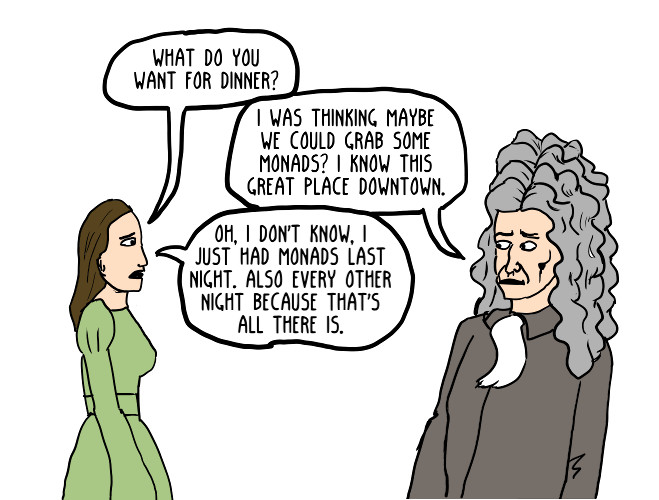
\includegraphics[scale=.7]{monadsForDinner.jpg}\\
	%\vspace{.3cm}
	%\includegraphics[scale=.3]{intbn}
\end{figure}	
\end{center}
		
	\end{titlepage}


\frontmatter
	\thispagestyle{empty}\doclicenseThis
	Cover image \copyright \href{http://existentialcomics.com/comic/other/10}{\ Existential comics}
	\tableofcontents
	
	\mainmatter
	

	
	\chapter*{Categorical preliminaries}
	\begin{defn}[Categories]
		A \emph{category} $\C$ consists of:
		\begin{enumerate}
			\item a collection of objects $\Ob(\C)$;
			\item a collection of arrows $\Ar(\C)$;
			\item two maps $\dom,\cod\colon\Ar(\C)\rightarrow\Ob(\C)$;
			\item a map $\id_{-}\colon\Ob(\C)\rightarrow\Ar(\C)$ with $\dom(\id_{c})=c=\cod(\id_{c})$;
			\item for every $f,g\in\Ar(\C)$ such that $\cod(f)=\dom(g)$ a unique composite morphism $gf$ such that $\cod(gf)=\cod(g)$, $\dom(gf)=\dom(f)$.
		\end{enumerate}
	This data has to satisfy the following axioms
		\begin{enumerate}
			\item given $f\in\Ar(\C)$, $c=\dom(f)$ and $c'=\cod(f)$, $\id_{c'}f=f=\id_{c}$, that is the composition is unital;
			\item given a composable triple $f,g,h\in\Ar(\C)$, $h(gf)=(hg)f$, that is the composition is associative.
		\end{enumerate}
		An arrow $f$ such that $c=\dom(f)$ and $c'=\cod(f)$ is denoted $f\colon c\rightarrow c'$.
	\end{defn}
	
	\begin{defn}[Functors]
		
	\end{defn}
	
	\begin{defn}[Full functors, faithful functor]
		
	\end{defn}
	
	\begin{defn}[Natural transformations]
		
	\end{defn}
	
	\begin{defn}[Equivalent functors]
	\end{defn}
	
	\begin{defn}[Representable Functors]
		
	\end{defn}
	
	\begin{defn}[Whiskering]
		
	\end{defn}
	
	\begin{defn}[Horizontal and vertical composition of nat.transf.]
		
	\end{defn}
	
	\begin{defn}[adjunctions]
		
	\end{defn}
	
	\begin{lemma}[Yoneda]
		
	\end{lemma}
	\begin{proof}
		
	\end{proof}

\noindent We will denote by $\yo$  (the kana for ``Yo") the Yoneda embedding $\C\hookrightarrow\Set^{\C^{\op}}$.
	
	\chapter{Monads and algebras}
	
	Throughout mathematics we encounter structures defined by some action morphisms. Here we give some examples.
	
	\begin{exmp}
		Given a group $G$, we may consider a $G$-set $X$ described by an action map $G\times X\rightarrow X$.
	\end{exmp}
	\begin{exmp}
		Given an abelian group $M$ and a ring $R$, we can get an $R$-module $M$ by fixing a group homomorphism $R\otimes_{\Z} M\rightarrow M$.
	\end{exmp}
	\begin{exmp}
		Given a monoid $M$ in $\Set$, we get a map $\Pi_{k=1}^n M\rightarrow M$, $(m_1,\ldots,m_n)\mapsto ((\ldots ((m_1m_2)m_3)\ldots )m_{n-1}) m_n$. This induces an action map from $W(M)=\amalg_{n\in\N}\Pi_{k=1}^n M$, the set of words on $M$, to $M$.
	\end{exmp}
	\begin{exmp}\label{ultrafilters}
		Given a set $X$, let $\mathcal{U}X$ be the set of ultrafilters on it. Any compact T2 topology on $X$ allows us to see each ultrafilter as a system of neighborhoods of a unique point in $X$, hence it gives us a unique map $\mathcal{U}X\rightarrow X$ sending each ultrafilter to the respective point.
	\end{exmp}
	\begin{exmp}
		Given a directed graph $D=(V,E,\hspace{-1.5mm}\begin{tikzcd}
		E\hspace{-1.5mm}\arrow[r, "t" description,  shift right=.5ex, shorten <= .3em, shorten >= .3em]  \arrow[r, "s" description, shift left=1ex, shorten <= .3em, shorten >= .3em] & \hspace{-1.5mm}V
		\end{tikzcd}\hspace{-1.5mm})$, we can create its free category $FD$, where the objects are the vertices and $FD(v,w)=\{\text{finite paths } v\rightarrow\ldots\rightarrow w\}$. We set $\id_v$ to be the path of length 0, while composition is just the concatenation of paths.
		
		In particular, if $D$ is the directed graph with $V=\{0,\ldots,n\}$ and an edge $j\rightarrow k$ if and only if $k=j+1$, we have $FD\cong [n]$.
		
		If $D=\{*\}$ and $E=\{*\rightarrow *\}$, then $FD(*,*)\cong\N$.
		
		Given a small category $\C$, we may consider the underlying graph $U\C=D$ with $V=\Ob(\C)$, $E=\Ar(\C)$, $s=\dom$ and $t=\cod$. We get then an action map $UFU\C\rightarrow U\C$ sending a finite path to its composite. This map is a morphism of directed graphs.
	\end{exmp}

	Notice that we always have a category $\C$ and some functor $T\colon\C\rightarrow\C$ with an action map $T\C\rightarrow\C$. How can we see all of these examples as specific instances of a general phenomenon?
	
	\begin{defn}
		A \emph{monad} on a category $\C$ is a triple $(T,\mu,\eta)$ where $T\colon\C\rightarrow\C$ is a functor, while $\mu\colon T^2\Rightarrow T$ and $\eta\colon\id_{\C}\Rightarrow T$ are natural transformations such that the following diagrams commute.
		
		\[
			\begin{tikzcd}
				T^3\ar["\mu T"', Rightarrow]{d}\ar["T\mu", Rightarrow]{r}
				& T^2\ar["\mu", Rightarrow]{d} \\
				T^2\ar["\mu"', Rightarrow]{r}
				& T
			\end{tikzcd}
			\quad\quad
			\begin{tikzcd}
				T\ar["\eta T", Rightarrow]{r}\ar[equal]{dr}
				& T^2\ar["\mu", Rightarrow]{d}\ar["T\eta", Leftarrow]{r}
				& T\ar[equal]{dl} \\
				& T
			\end{tikzcd}
		\]
		
		$\mu$ is called the \emph{multiplicative map}, while $\eta$ is the \emph{unit} of $T$.
		
		The commutativity of the first diagram is equivalent to stating that the following two diagrams are equal.
		\begin{center}
		\begin{minipage}{0.3\linewidth}
			\begin{tikzcd}[row sep=1cm, column sep=1cm]
				&\C\ar[d, Rightarrow, shorten <= 1em, shorten >= 1em, "\mu"]\ar[r, "T"]\ar[drr, bend right=26, "T"description]
				&\C\ar[dr, "T"]\ar[d, Rightarrow, yshift=1ex, shorten <= 1em, shorten >= 1em, "\mu"]\\
				\C
				\ar[rrr, "T"'] 
				\ar[ur, , "T"]
				&\phantom{.} &\phantom{.}&\C
			\end{tikzcd}
		\end{minipage}
		\hspace{1cm}
				=
		\hspace{.2cm}
		\begin{minipage}{0.3\linewidth}
			\begin{tikzcd}[row sep=1cm, column sep=1cm]
				&\C\ar[d, Rightarrow, yshift=1ex, shorten <= 1em, shorten >= 1em, "\mu"]\ar[r, "T"]
				&\C\ar[d, Rightarrow, shorten <= 1em, shorten >= 1em, "\mu"]\ar[dr, "T"]\\
				\C\ar[urr, bend right=26, "T"'description]
				\ar[rrr, "T"'] 
				\ar[ur, , "T"]
				&\phantom{.} &\phantom{.}&\C
			\end{tikzcd}
		\end{minipage}
		\end{center}
	\end{defn}

On the other hand, the second diagram can be rephrased as follows:
\begin{center}
	
	\begin{minipage}{0.3\linewidth}
		\begin{tikzcd}[row sep=1cm, column sep=1cm]
		& \C \arrow[d, Rightarrow, shift left=.5ex, shorten <= 1em, shorten >= 1em, "\mu"]\arrow[d, Rightarrow, shift right=5.8ex, shorten <= 1em, shorten >= 1em, "\eta"]\arrow[rd, "T"] &   \\
		\C \arrow[rr, "T"', ""{name=A}] \arrow[ru, bend right, "T"'description, ""{name=T}] \arrow[ru, bend left, equal, ""{name=U}] &    \phantom{.}          & \C
		%\arrow[Rightarrow, from=U, to=D]
		\end{tikzcd}
		
	\end{minipage}
	=
	\hspace{.4cm}
	\begin{minipage}{0.3\linewidth}
		\begin{tikzcd}[row sep=1cm, column sep=1cm]
		\C \arrow[d, bend right, "T"'] \arrow[d, bend left, "T"] \\
		\C                                           
		\end{tikzcd}
	\end{minipage}
	\hspace{-4.5cm}
	=
	\hspace{1cm}
	=
	\hspace{.6cm}
	\begin{minipage}{0.3\linewidth}
		\begin{tikzcd}[row sep=1cm, column sep=1cm]
		& \C \arrow[d, Rightarrow, shift right=1.2ex, shorten <= 1em, shorten >= 1em, "\mu"]\arrow[d, Rightarrow, shift left=5.8ex, shorten <= 1em, shorten >= 1em, "\eta"] \arrow[rd, bend right, "T"'description, ""{name=T}] \arrow[rd, bend left, equal, ""{name=U}] &   \\
		\C \arrow[rr, "T"', ""{name=A}] \arrow[ru, "T", ""{name=B}] &\phantom{.}   & \C		\end{tikzcd}
	\end{minipage}
\end{center}

	A monad naturally defines other algebraic structures, which we now introduce.
	
	\begin{defn}
		Given a monad $(T,\mu,\eta)$, a \emph{$T$-algebra} or \emph{$T$-module} is a pair $(a,\alpha)$, where $a\in\Ob(\C)$ and $\alpha\colon Ta\rightarrow a$ is such that the following diagrams commute.
		\[	
			\begin{tikzcd}
				T^2 a\ar["\mu_{a}"']{d}\ar["T\alpha"]{r}
				& Ta\ar["\alpha"]{d} \\
				Ta\ar["\alpha"']{r}
				& a
			\end{tikzcd}
			\quad\quad
			\begin{tikzcd}
				a\ar[equal, swap]{dr}\ar["\eta_{a}"]{r}
				& Ta\ar["\alpha"]{d} \\
				& a
			\end{tikzcd}
		\]
	\end{defn}

	\begin{defn}
		A \emph{morphism of $T$-algebras} $(a,\alpha)\rightarrow (b,\beta)$ is a morphism $f\colon a\rightarrow b$ such that the following diagram commutes:
		\[
			\begin{tikzcd}
				Ta\arrow["\alpha"']{d}\arrow["Tf"]{r}
				& Tb\arrow["\beta"]{d} \\
				a\arrow["f"']{r}
				& b
			\end{tikzcd}
		\]
	\end{defn}

		
	$T$-algebras form a category $T\Alg$, which has a natural forgetful functor $U^T\colon T\Alg\rightarrow\C$.
	
	We now show how to recover the examples previously given with this language.
	
	\begin{exmp}
		\begin{align*}
			T=G\times - \colon&\ \Set \rightarrow\Set \\
			\mu_A\colon&\ G\times (G\times A) \rightarrow G\times A \\
			&\ (g,(h,a)) \mapsto (gh,a) \\
			\eta_A\colon&\ A \rightarrow G\times A \\
			&\ a \mapsto (e,a)
		\end{align*}
		is a monad and $(A,\alpha)$ is a $T$-algebra if and only if $A$ is a $G$-set. It follows that $T\Alg\cong G\mbox{-}\Set$.
	\end{exmp}

	\begin{exmp}
		Given a ring $R$, $T=R\otimes_{\Z}-\colon \Ab\rightarrow \Ab$ is a monad when considered with the following natural transformations:
		\begin{align*}
			\mu_{-}\colon &\ R\otimes_{\Z}(R\otimes_{\Z}-)\cong (R\otimes_{\Z}R)\otimes_{\Z}-\Rightarrow R\otimes_{\Z}- \\
			\eta_-\colon &\ -\cong\Z\otimes_{\Z}-\Rightarrow R\otimes_{\Z}-
		\end{align*}
	We have that $(R\otimes_{\Z}-)\Alg\cong\Mod_R$.
	\end{exmp}

	\begin{exmp}
		Consider $W\colon\Set\rightarrow\Set$ given by $WX=\amalg_{n\in\N}\Pi_{k=1}^n X$. Multiplication $\mu_X\colon WWX\rightarrow WX$ is given by concatenation of words, while the unit $\eta_X\colon X\rightarrow WX$ is just $x\mapsto (x)$. With this, $W\Alg\cong \text{Mon}(\Set)$.
	\end{exmp}

	\begin{exmp}
		The functor $\mathcal{U}$ defined in Example \ref{ultrafilters}, equipped with suitable natural transformations, is a monad on $\Set$ and $\mathcal{U}\Alg\cong \CHTop$, the category of compact T2 spaces.
	\end{exmp}

	\begin{exmp}
		The free-forgetful adjunction $F\dashv U$ between categories and directed graphs induces a monad on the latter, with $UF\Alg\cong\Cat$.
	\end{exmp}

	\section{Monadic functors}
	
	Now that we have introduced these structures, our aim is to characterize \emph{monadic functors}, that is functors $U\colon\A\rightarrow\C$ which are equivalent to $U^T\colon T\Alg\rightarrow\C$ for some monad $(T,\mu,\eta)$ on $\C$.

	First of all, notice that $U^T$ is faithful by construction, hence $U$ must be faithful, but more is true.
	
	\begin{lemma}
		The functor $U^T$ is conservative, that is if $U^Tf$ is an isomorphism then $f$ is an isomorphism of $T$-algebras.
	\end{lemma}
	\begin{proof}
		Suppose that $g$ is the inverse of $f\colon a\rightarrow b$ and $f$ is a morphism $(a,\alpha)\rightarrow (b,\beta)$. We only need to prove that the square on the left commutes, that is $g\beta=\alpha Tg$:
		\[
			\begin{tikzcd}
				Tb\arrow["\beta"']{d}\arrow["Tg"]{r}
				& Ta\arrow["\alpha"']{d}\arrow["Tf"]{r}
				& Tb\arrow["\beta"]{d} \\
				b\arrow["g"']{r}
				& a\arrow["f"']{r}
				& b
			\end{tikzcd}
		\]
		
	We see that $fg\beta=\beta$ and $f\alpha Tg=\beta Tf Tg=\beta T(fg)=\beta T\id_b=\beta$, hence the thesis.
	\end{proof}
    \begin{rmk}
     Notice that the forgetful functor $U\colon\Top\to\Set$ can't be monadic since it does not reflect isomorphisms. However, if we restrict it to the full subcategory of $\Top$ spanned by compact Hausdorff spaces we indeed obtain a monadic functor.
    \end{rmk}
	\begin{prop}
		The functor $U^T\colon T\Alg\rightarrow\C$ has a left adjoint $F^T\colon\C\rightarrow T\Alg$ such that $F^Tc=(Tc,\mu_{c})$, $F^Tf\colon(Tc,\mu_{c})\xrightarrow{Tf} (Td,\mu_{d})$ and $U^TF^T=T$. Furthermore, the unit of this adjunction is given by $\eta$ and the counit has components $\epsilon_{(a,\alpha)}=\alpha\colon(Ta,\mu_a)\to(a,\alpha)$.
	\end{prop}
\begin{proof}
	\begin{enumerate}[label=(\roman*)]
		\item To show that $(Tc, \mu_c)$ is a $T$-algebra we need the following diagrams to be commutative.
		\[
		\begin{tikzcd}
		T^3c\ar["\mu_{Tc}"', rightarrow]{d}\ar["T\mu_c", rightarrow]{r}
		& T^2c\ar["\mu_c", rightarrow]{d} \\
		T^2c\ar["\mu_c"', rightarrow]{r}
		& Tc
		\end{tikzcd}
		\quad\quad
		\begin{tikzcd}
		Tc\ar["\eta_{Tc}",rightarrow]{r}\ar[equal]{dr}
		& T^2c\ar["\mu_c", rightarrow]{d}
		\\
		& Tc
		\end{tikzcd}
		\]
		These are exactly the associativity and one of the unit laws for $(T, \mu, \eta)$.
	\item For every $f\colon c\to c'$, $Tf$ is a morphism of algebras $(Tc,\mu_c)\to(Tc', \mu_{c'})$ because the diagram 
		\[
	\begin{tikzcd}
	T^2c\ar["\mu_{c}"', rightarrow]{d}\ar["T^2f", rightarrow]{r}
	& T^2c'\ar["\mu_{c'}", rightarrow]{d} \\
	Tc\ar["Tf"', rightarrow]{r}
	& Tc'
	\end{tikzcd}
		\]
	is commutative by naturality of $\mu$, hence $F^T$ is defined on morphisms. It is a functor by functoriality of $T$.
	\item The unit is natural by assumption. We claim that $\epsilon_{(a,\alpha)}=\alpha$ is a morphism of algebras $$F^TU^T(a,\alpha)=F^Ta=(Ta,\mu_a) \to \id_{T\Alg}(a,\alpha)=(a,\alpha)$$ and $\epsilon$ is a natural transformation $F^TU^T\Rightarrow\id_{T\Alg}$. Let's check it. We know that $\alpha$ is a morphism of algebras if and only if 
	\[	
	\begin{tikzcd}
	T^2 a\ar["\mu_{a}"']{d}\ar["T\alpha"]{r}
	& Ta\ar["\alpha"]{d} \\
	Ta\ar["\alpha"']{r}
	& a
	\end{tikzcd}
	\]
	is commutative, but this is one of the two $T$-algebra axioms! Moreover, to prove that $\epsilon$ is natural, we need to show that
		\[	
	\begin{tikzcd}
	(Ta,\mu_a) \ar["Tf"']{d}\ar["\alpha=\epsilon_{(a,\alpha)}"]{r}
	& (a,\alpha)\ar["f"]{d} \\
	(Tb,\mu_b)\ar["\beta=\epsilon_{(b,\beta)}"']{r}
	& (b,\beta)
	\end{tikzcd}
	\]
	is commutative, but this is the axiom for $f$ to be a morphism of $T$-algebras! 
	\item It remains to check the two triangular identities $\epsilon F^T \cdot F^T\eta=\id_{F^T}$ and $U^T\epsilon\cdot\eta U^T=\id_{U^T}$. These are to be checked on the components at $c$ and $(a, \alpha)$, respectively.
	\[
		\begin{tikzcd}
	(Tc,\mu_c)\ar["T\eta_{c}",rightarrow]{r}\ar[equal]{dr}
	& (T^2c,\mu_{Tc})\ar["\mu_{Tc}", rightarrow]{d}
	\\
	& (Tc,\mu_c)
	\end{tikzcd}	\quad\quad
	\begin{tikzcd}
	a\ar["\eta_a",rightarrow]{r}\ar[equal]{dr}
	& Ta\ar["\alpha", rightarrow]{d}
	\\
	& a
	\end{tikzcd}
	\]
	The commutativity of these diagrams is ensured by the second unit law for a monad and the unit law for the $T$-algebra $(a,\alpha)$ respectively. \qedhere
	\end{enumerate}
\end{proof}
\begin{defn}
Given a monad $(T,\mu,\eta)$, $T$-algebras of the form $(Tc, \mu_c)$ are called \emph{free $T$-algebras}.
\end{defn}
Thanks to the proposition above we can prove that, given a monad $T$, we can always find an adjunction that generates it. Actually, the converse holds too.
\begin{prop}
If $U\colon\D\to\C$ has a left adjoint $F$ with unit $\eta$ and counit $\epsilon$, then $(UF,U\epsilon F,\eta)$ is a monad on $\C$. Also, if $(T,\mu,\eta)$ is a monad on $\C$, then $(U^TF^T,U^T\epsilon F^T,\eta)=(T,\mu,\eta)$. 
\end{prop}
\begin{proof}
Let us check the axioms. First of all, the associativity holds due to the following equations.
\flushleft
\begin{center}
	\begin{tikzcd}[row sep=.55cm, column sep=.55cm]
		&&\C\arrow[rd, "F"]\ar[d, Rightarrow, shorten <= .5em, shorten >= .5em, "\epsilon"']&&&&&&\C\arrow[rd, "F"]\ar[d, Rightarrow, shorten <= .5em, shorten >= .5em, "\epsilon"'] &&\\
		\C\arrow[r, "F"]&\D\arrow[ru, "U"] \arrow[rr, equal] &\phantom{.}& \D \arrow[r, "U"] & \C \arrow[r, "F"] & \D \arrow[r, "U"] & \C  \arrow[r, "F"] &\D\arrow[ru, "U"] \arrow[rr, equal] &\phantom{.}& \D \arrow[r, "U"] & \C
		\end{tikzcd}\\
		\vspace{5mm}
				=				
		\begin{tikzcd}
		&&\C\arrow[rd, "F"]\ar[d, Rightarrow, shorten <= .5em, shorten >= .5em, "\epsilon"']&&\C\arrow[rd, "F"]\ar[d, Rightarrow, shorten <= .5em, shorten >= .5em, "\epsilon"']\\
		\C\arrow[r, "F"]&\D\arrow[ru, "U"] \arrow[rr, equal] &\phantom{.}& \D\arrow[ru, "U"] \arrow[rr, equal] &\phantom{.}& \D\arrow[r, "U"]&\C
		\end{tikzcd}\\
		\vspace{5mm}
		    =
		\begin{tikzcd}[row sep=.55cm, column sep=.55cm]
		&            &            &                                    &\C  \arrow[rd, "F"]\ar[d, Rightarrow, shorten <= .5em, shorten >= .5em, "\epsilon"'] &            &            &                                    &  \C\arrow[rd, "F"]\ar[d, Rightarrow, shorten <= .5em, shorten >= .5em, "\epsilon"'] &            &  \\
		\C\arrow[r, "F"] & \D \arrow[r, "U"] & \C  \arrow[r, "F"] &  \D\arrow[ru, "U"] \arrow[rr, equal] &  \phantom{.}           &\D  \arrow[r, "U"] &\C  \arrow[r, "F"] & \D \arrow[ru, "U"] \arrow[rr, equal] &\phantom{.}             &\D  \arrow[r, "U"] & \C
		\end{tikzcd}
\end{center}
Unit laws:
\[
\begin{tikzcd}
&         \arrow[d, Rightarrow, yshift=1ex, shorten <= .5em, shorten >= .01em, "\eta"']    &\C \arrow[d, Rightarrow, shorten <= .5em, shorten >= .5em, "\epsilon"']  \arrow[rd, "F"] &            &  \\
\C\arrow[r, "F"] \arrow[rru, bend left, equal] &\D  \arrow[ru, "U"] \arrow[rr, equal] &  \phantom{.}           &\D  \arrow[r, "U"] & \C
\end{tikzcd}
\]
is equal to $1_{UF}$, since $\epsilon F\cdot F\eta=1_F$ by one of the triangular identities of the adjunction $F\dashv U$. Similarly,
\[
\begin{tikzcd}
&            &\C \arrow[d, Rightarrow, shorten <= .5em, shorten >= .5em, "\epsilon"']  \arrow[rd, "F"]\arrow[rrd, bend left, equal] &  \arrow[d, Rightarrow, yshift=1ex, shorten <= .5em, shorten >= .01em, "\eta"']           &  \\
\C\arrow[r, "F"]  &\D  \arrow[ru, "U"] \arrow[rr, equal] &  \phantom{.}           &\D  \arrow[r, "U"] & \C
\end{tikzcd}
\] 
is equal to $1_{UF}$.

The rest follows from the explicit description of unit and counit of the adjunction $F^T\dashv U^T$, in fact 
$U^T\epsilon F^Tc=U^T\epsilon_{(Tc, \mu_c)}=\mu_c$.
\end{proof}

\begin{exmp}[Interesting adjunction, boring monad] Let us consider the adjunction $U\colon\mathbf{Top}\rightleftarrows\Set\colon\mathsf{Disc}\eqqcolon F$, whose left adjoint assigns to every set $X$ the discrete topological space $FX=(X, 2^X)$.
It's immediate to see that $UFX=X$, hence $UF=\id_\Set$. How many natural transformations $\id_\Set=UF\xRightarrow{\alpha} UF=\id_\Set$ are there?
We know that $\id_\Set\cong\Hom(*,-)$, so $\text{Nat}(\id_\Set, \id_\Set)\cong\text{Nat}(\Hom(*,-),\Hom(*,-))\cong\Hom(*,*)=\{\id_*\}$ by Yoneda, hence $\alpha=\id$. Therefore $(UF,U\epsilon F, \eta)=(\id_\Set, \id, \id)$
\end{exmp}
\begin{exmp}
If $S$ is a set, then $\Set(S,-)\colon\Set\to\Set$ is right adjoint to $S\times-\colon\Set\to\Set$, so we get a monad $X\mapsto\Set(S,S\times X)$. This is called the \emph{state monad} and it is important in Computer Science.
\end{exmp}


\section{The category of $T$-actions}

Given an adjunction$\begin{tikzcd}F\colon\cC\ar[r, shift left = .4em, above, ""{name=F}] &\cD\colon U,\ar[l, shift left = .4em, below, ""{name=U}]\ar[from=F, to=U, symbol=\dashv]\end{tikzcd}$ there is always a comparison morphism $\D\xrightarrow{\overline{U}}UF\Alg$ such that 
\[
\begin{tikzcd}[column sep=tiny]
\D\ar["\overline{U}"]{rr}\ar["U"']{dr}
&& UF\Alg\ar["U^{UF}", rightarrow]{dl}
\\
& \C
\end{tikzcd}
\]
commutes. We set $\overline{U}f=(Ud,UFUd\xrightarrow{U\epsilon_d}Ud)=(Ud, U\epsilon_d)$. More generally, for a given functor $G\colon\D\rightarrow\C$ we can ask what do we need to get a lift $\overline{G}\colon\D\to T\Alg$. To get there, we will need a few more definitions and lemmas.

Just like a monad $(T,\mu,\eta)$ defines a category $T\Alg$, it also allows us to construct another category from functors $\D\rightarrow\C$.

\begin{defn}
	Given a monad $(T,\mu,\eta)$ on a category $\C$ and fixed another category $\D$, a \emph{$T$-action} on a functor $G\colon\D\to\C$ is a natural transformation $\gamma\colon TG\Rightarrow G$ such that the diagrams
	\[
		\begin{tikzcd}
			T^2G\ar["\mu G"', Rightarrow]{d}\ar["T\gamma", 	Rightarrow]{r}
			& TG\ar["\gamma", Rightarrow]{d} \\
			TG\ar["\gamma"', Rightarrow]{r}
			& G
		\end{tikzcd}
		\quad\quad
		\begin{tikzcd}
			G\ar["\eta G", Rightarrow]{r}\ar[equal]{dr}
			& TG\ar["\gamma", Rightarrow]{d}\\
			& G
		\end{tikzcd}
	\]
		commute.
	
		A \emph{morphism of $T$-actions} $(G,\gamma)\xRightarrow{\varphi}(K,\kappa)$ is a natural transformation $\varphi\colon G\Rightarrow K$ such that
\[
\begin{tikzcd}
	TG\ar["T\varphi", Rightarrow]{r}\ar["\gamma"', Rightarrow]{d}
		& TK\ar["\kappa", Rightarrow]{d}\\
		G\ar[r, Rightarrow, "\varphi"']& K 
		\end{tikzcd}
		\]
		commutes.
	
		Up to size, $T$-actions and their morphisms assemble into a category $T\mbox{-}\mathsf{Act}(\D)$.
	\end{defn}

	

\begin{exmp}
	The functor $U^T\colon T\Alg\rightarrow\C$ has a $T$-action given by $\alpha\colon TU^T\Rightarrow U^T$, where $\alpha_{(b,\beta)}\coloneqq\beta\colon Tb\rightarrow b$.
\end{exmp}

\begin{exmp}
	Given an adjunction$\begin{tikzcd}F\colon\cC\ar[r, shift left = .4em, above, ""{name=F}] &\cD\colon U\ar[l, shift left = .4em, below, ""{name=U}]\ar[from=F, to=U, symbol=\dashv]\end{tikzcd}$with unit $\eta\colon\id_{\C}\Rightarrow UF$ and counit $\epsilon\colon FU\Rightarrow\id_{\D}$, we get a monad on $(UF,U\epsilon F,\eta)$ on $\C$. We have then a $UF$-action $U\epsilon\colon UFU\Rightarrow U$, where the axioms follow from the triangular identities and the naturality of $U\epsilon$.
\end{exmp}

\begin{prop}
	$(U^T,\alpha)$ is the universal $T$-action, that is for any category $\D$ the functor $\Cat(\D,T\Alg)\rightarrow T\mbox{-}\mathsf{Act}(\D)$ sending $G$ to $(U^TG,\alpha G)$ and $\beta\colon G\Rightarrow H$ to $U^T\beta\colon(U^TG,\alpha G)\Rightarrow (U^TH,\alpha H)$ is an isomorphism of categories.
\end{prop}

\begin{proof}
	In other words, for every $T$-action $(G,\gamma)$ there exists a unique lift $\overline{G}\colon\D\rightarrow T\Alg$ such that $(U^T\overline{G},\alpha\overline{G})=(G,\gamma)$ and for every $\phi\colon(G,\gamma)\Rightarrow (K,\kappa)$ there is a unique $\overline{\phi}\colon\overline{G}\Rightarrow\overline{K}$ with $U^T\overline{\phi}=\phi$.
	
	It is enough to set $\overline{G}d\coloneqq(Gd,\gamma_d)$ on objects, $\overline{G}f\coloneqq Gf$ on morphisms, $\overline{\phi}_d\coloneqq\phi_d$ and check the axioms.
	\[
		\begin{tikzcd}
			\D\ar[r, dashed, "\exists!\overline{G}"]\ar[dr, swap, "G"]
			& T\Alg\ar[d, "U^T"] \\
			& \C                  
		\end{tikzcd}    
	\]			
\end{proof}

Following the construction in this proof, from the last example we get the comparison functor for the adjunction $F\dashv U$. In particular, $\overline{U}d=(Ud,U\epsilon_d)$. Furthermore, this means that $U\colon\Top\rightarrow\Set$ factors through identities.


\section{Limits and colimits in the category of algebras}

We have shown that the forgetful functor $U^T\colon T\Alg\rightarrow\C$ is a right adjoint and as such it preserves limits. However, more is true.

\begin{prop}\label{create lims}
	For any monad $(T,\mu,\eta)$ on $\C$, the forgetful functor $U^T\colon T\Alg\rightarrow\C$ strictly creates limits.
\end{prop}

\begin{proof}
	This statement means that, for any diagram $D\colon\cI\rightarrow T\Alg$ such that $U^TD\colon\cI\rightarrow\C$ has a limit $(l,\kappa_i)$ in $\C$, there is a unique $T$-algebra structure $\lambda\colon Tl\rightarrow l$ such that $\kappa_i$ is a morphism of $T$-algebras for all $i\in\cI$ and this makes $((l,\lambda),\kappa_i)$ into a limit of $D$.
	
	Now we begin the proof.
	
	First of all, remember that $D\phi\colon D_i\rightarrow D_j$ is a morphism of $T$-algebras for all $\phi\colon i\rightarrow j$ by assumption, hence the morphisms $\delta_i T\kappa_i\colon Tl\rightarrow D_i$ define a cone over $D$, where $\delta_i$ is the $T$-algebra structure on $D_i$. By the universal property of the limit, there is a unique morphism $\lambda\colon Tl\rightarrow l$ making the following diagram commute for all $i$.
	\[
	\begin{tikzcd}
	Tl\ar[d, dashed, "\lambda"'] \ar[r, "T\kappa_i"]
	& TD_i\ar[d, "\delta_i"]\\
	 l\ar[r, "\kappa_i"']
	& D_i
	\end{tikzcd}
	\]	
	This tells us that, if the limit $((l,\lambda),\kappa_i)$ of $D$ exists, it is unique. We have to check that $(l,\lambda)$ is a $T$-algebra.
	
	Notice that for all $i$ all of the faces of the following diagrams, except for possibly the top ones, commute.
	
	\[
		\begin{tikzcd}
			& Tl\ar[drr, "\lambda"]\ar[ddd, "T\kappa_i" near start] \\
			T^2l\ar[ur, "T\lambda"]\ar[drr, crossing over, "\mu_l" near start, swap]\ar[ddd, "T^2\kappa_i"']
			&&& l\ar[ddd, "\kappa_i"] \\
			&& Tl\ar[ur, "\lambda"]%\ar[ddd, "T\kappa_i" near start] 
			\\
			& TD_i\ar[drr, swap, "\delta_i" near start] \\
			T^2D_i\ar[ur, "T\delta_i"]\ar[drr, "\mu_{D_i}"']
			&&& D_i \\
			&& TD_i\ar[ur, "\delta_i"'] \ar[from=uuu,crossing over,  "T\kappa_i" near start]
		\end{tikzcd}
		\quad\quad
		\begin{tikzcd}
			& Tl\ar[dr, "\lambda"]\ar[dd, "T\kappa_i" near end] \\
			l\ar[ur, "\eta_l"]\ar[rr, crossing over, equal]\ar[dd, swap, "\kappa_i"]
			&& l\ar[dd, "\kappa_i"] \\
			& TD_i\ar[dr, "\delta_i"] \\
			D_i\ar[ur, "\eta_{D_i}"]\ar[rr, equal]
			&& D_i
		\end{tikzcd}
	\]
	
	Since the $\kappa_i$ are jointly monic, the upper face commutes and therefore $(l,\lambda)$ is a $T$-algebra. It remains to check that $((l,\lambda),\kappa_i)$ factors every other cone over $D$.
	
	Let $\gamma_i\colon(x,\zeta)\rightarrow (D_i,\delta_i)$ be a cone over $D$. Then, there is a unique $f\colon x\rightarrow l$ in $\C$ such that $\kappa_if=\gamma_i$. We only have to show that $f$ is a morphism of $T$-algebras $(x,\zeta)\rightarrow (l,\lambda)$.
	
	Consider the following diagram and notice that the outer square, the one on the right and the two triangles commute, hence the square on the left commutes as well since the $\kappa_i$ are jointly monic.
	
	\[
		\begin{tikzcd}
			Tx\ar[rr, bend left, "T\gamma_i"]\ar[r, swap, "Tf"]\ar[d, "\zeta"]
			& Tl\ar[r, swap, "T\kappa_i"]\ar[d, "\lambda"]
			& TD_i\ar[d, "\delta_i"] \\
			x\ar[r, "f"]\ar[rr, bend right, swap, "\gamma_i"]
			& l\ar[r, "\kappa_i"]
			& D_i
		\end{tikzcd}
	\]
\end{proof}

A similar statement holds for colimits.

\begin{prop}\label{create colims}
Given a monad $(T,\mu,\eta)$ on $\C$, the forgetful functor $U^T\colon T\Alg\rightarrow\C$ strictly creates any colimit preserved by both $T$ and $T^2$.
\end{prop}

\begin{proof}
	Similarly to the dual situation, this means that for any diagram $D\colon I\rightarrow T\Alg$ such that $U^TD\colon I\rightarrow\C$ has a colimit $(c,\kappa_i)$ preserved by both $T$ and $T^2$, there is a unique $T$-algebra structure $\lambda\colon Tc\rightarrow c$ such that $\kappa_i$ is a morphism of $T$-algebras for all $i\in I$. This makes $((c,\lambda),\kappa_i)$ into a colimit of $D$.
	
	The proof is essentially dual to the one given earlier, in the sense that we find again a unique $\lambda\colon Tc\rightarrow c$ using the universal property of the colimit $(Tc,T\kappa_i)$ of $TD$.
	\[
		\begin{tikzcd}
			TD_i\ar[r, "T\kappa_i"]\ar[d, "\delta_i"']
			& Tc\ar[d, dashed, "\lambda"] \\
			D_i\ar[r, "\kappa_i"']
			& c
		\end{tikzcd}
	\]
	To check that $(c,\lambda)$ is an algebra we use the universal property of $(T^2c,T^2\kappa_i)$, for $\mu$, and the one of $(c,\kappa_i)$, for $\eta$.
\end{proof}

\begin{rmk}
	The same statements hold for monadic functors, except for the fact that they might not create limits and colimits strictly since they are just equivalent to a $U^T$.
\end{rmk}

\begin{rmk}
	If $T$ is a monad on a complete category $\C$, then $T\Alg$ is complete. If $\C$ is cocomplete and $T$ is cocontinuous, then $T\Alg$ is cocomplete.
\end{rmk}

\begin{exmp}
	Let $\C$ be a small category. There is a cocontinuous monad on the category of $\Ob(\C)$-indexed collections of sets whose category of algebras is the functor category $[\C,\Set]$. The underlying endofunctor of this monad is defined as 
	\begin{align*}
	T\colon[\Ob(\C),\Set]&\to[\Ob(\C),\Set] \\
	(X_c)_{c\in\C}&\mapsto \left(\coprod_{d\in\C}\C(d,c)\times X_d\right)_{c\in\C}
	\end{align*}
	Since $[\Ob(\C),\Set]$ is complete and cocomplete, so is $[\C,\Set]$ (with limits and colimits computed pointwise).
\end{exmp}
 
\section{Beck’s monadicity theorem}

The final ingredient we need to give a characterization of monadic functors is the observation that $T$-algebras admit canonical presentations using free algebras.

\begin{exmp}
	Pick an epimorphism $F\twoheadrightarrow G$ in the category of groups $\mathbf{Grp}$, where $F$ is a free group. The kernel of this homomorphism defines a (normal) subgroup $K$ of $F$, giving rise to the sequence $K\rightarrowtail F\twoheadrightarrow G$. We can take another epimorphism $F'\twoheadrightarrow K$, with $F'$ again a free group, which presents $G$ as the cokernel of some morphism $F'\to F$ between free groups. This argument applies to rings, algebras, etc.
\end{exmp}

It is natural to ask if we can do this systematically for general $T$-algebras. Given $(a,\alpha)$ in $T\Alg$, we have $F^TU^T(a,\alpha)\to(a,\alpha)$, that is $(Ta,\mu_a)\xrightarrow{\alpha}(a,\alpha)$. A candidate\footnote{Think about free groups: in that case we take words on $Ta$.} for $F'$ would be $F^TU^T(Ta, \mu_a)=(T^2a, \mu_{Ta})$. Notice that 
\[
(T^2a,\mu_{Ta}) \doublerightarrow{T\alpha}{\mu_a}(Ta,\mu_a)\xrightarrow{\alpha}(a,\alpha)
\]
is a well defined diagram in $T\Alg$, with $\alpha\mu_a=\alpha T\alpha$. Moreover, this is a coequalizer. In order to use Proposition~\ref{create colims} to prove it that we need to check whether $U^T$ sends the diagram above into a coequalizer preserved by $T$ and $T^2$. In $\C$, we extend the diagram to
\[
\begin{tikzcd}
T^2a\arrow[r, shift left, "T\alpha"] \arrow[r, shift right, "\mu_a"']
&Ta  \arrow[r, "\alpha"] \arrow[l, bend left=49, swap, "\eta_{Ta}"'] & a \arrow[l, bend left=49, swap, "\eta_a"']
\end{tikzcd}
,\]
where the following equations hold true: $\alpha T\alpha=\alpha\mu_a$, $\alpha\eta_a=\id_a$, $\mu_a\eta_{Ta}=\id_{Ta}$ and $\eta_a\alpha=T\alpha\hspace{1mm}\eta_{Ta}$ by naturality. It is a particular case of a more general concept.
\begin{defn}
	A \emph{split coequalizer} is a diagram of the form
	\vspace*{-2.4mm}
	\[
	\begin{tikzcd}[ampersand replacement=\&]
	a\arrow[r, shift left, "f"] \arrow[r, shift right, "g"']
\& b \arrow[r, "h"] \arrow[l, bend left=49, "t"] \& c \arrow[l, bend left=49, "s"]
	\end{tikzcd}
	\]
	so that $hf=hg,\ hs=\id_c,\ gt=\id_b$, and $ft=sh$.
\end{defn}

\begin{prop}
In the above situation, 
\[
\begin{tikzcd}[ampersand replacement=\&]
a\arrow[r, shift left, "f"] \arrow[r, shift right, "g"']
\& b \arrow[r, "h"] \& c 
\end{tikzcd}
\] is a coequalizer. In particular, any functor preserves this coequalizer.
\end{prop}
\begin{proof}
Take $k\colon b\to d$ such that $kf=kg$ and define $\overline{k}\coloneqq ks$. Then we have
$$\overline{k}h=ksh=kft=kgt=k.$$
Uniqueness is clear since $h$ is a (split) epimorphism. 
\end{proof}
$T$ and $T^2$ preserve split coequalizers, so they preserve our coequalizer.
\begin{cor}
Let $T$ be a monad on $\C$ and $(a,\alpha)$ a $T$-algebra. Then 
\[
(T^2a,\mu_{Ta}) \doublerightarrow{T\alpha}{\mu_a}(Ta,\mu_a)\xrightarrow{\alpha}(a,\alpha)
\]
is a coequalizer in $T\Alg$, which $U^T\colon T\Alg\to\C$ sends to a split coequalizer in $\C$.
\end{cor}
\begin{proof}
We have already observed that the second statement holds, so that coeq$(U^T(T\alpha), U^T(\mu_a))$ is preserved by $T$ and $T^2$. Hence there exists a unique lift of the (split) coequalizer in $\C$ to a coequalizer in $T\Alg$. 
\end{proof}
Results like the previous one inspire us to look at the parallel pairs of morphisms in a category which are sent to split coequalizers or, to say it better, to a parallel pair of morphisms that can be extended to a split coequalizer diagram. This kind of pairs will be of crucial importance in the following.
\begin{defn}
Let $U\colon\D\to\C$ be a functor. A pair of morphisms $f,g\colon d\rightrightarrows d'$ in $\D$ is \emph{$U$-split} if $Uf,Ug\colon Ud\rightrightarrows Ud'$ is part of a split coequalizer in $\C$.
\end{defn} 
\begin{rmk}
$T\alpha,\mu_a\colon(T^2a,\mu_{Ta})\rightrightarrows(Ta,\mu_a)$ is a $U^T$-split pair. Moreover, $T\Alg$ has coequalizers of $U^T$-split pairs and $U^T$ preserves them. Hence, functors equivalent to $U^T$ satisfy three conditions:
\begin{enumerate}
	\item they have a left adjoint;
	\item they are conservative;
	\item $U$-split pairs have coequalizers which are preserved by $U$.
\end{enumerate}
\end{rmk}

\begin{teo}[Beck]\label{Beck} Let $U\colon\D\to\C$ be a right adjoint to $F\colon\C\to\D$. Let $(T=UF, U\epsilon F, \eta)$ be the induced monad and $\overline{U}\colon\D\to T\Alg$ be the comparison functor. 
	\begin{enumerate}
		\item If $\D$ has coequalizers of $U$-split pairs, then $\overline{U}$ has a left adjoint $\overline{F}\colon T\Alg\to\D$;
		\item if, in addition, $U$ preserves coequalizers of $U$-split pairs, the unit $\overline{\eta}\colon\id_{T\Alg}\Rightarrow\overline{U}\hspace{.5mm} \overline{F}$ is an isomorphism;
		\item if $U$ is also conservative, then $\overline{U}$ is an equivalence of categories.
	\end{enumerate}
	\end{teo}
	\begin{proof}
	\begin{enumerate}
	\item For each free $T$-algebra $(Ta,\mu_a)$ we have
	\begin{align*}
	T\Alg((Ta,\mu_a),\overline{U}-)&=T\Alg(F^Ta,\overline{U}-)\\
	&\cong\C(a, U^T\overline{U}-)\\
	&=\C(a,U-)\\
	&\cong\D(Fa,-),
	\end{align*} 
	therefore the value of $\overline{F}$ at $(Ta,\mu_a)$ has to be $Fa$. Since every $T$-algebra is a coequalizer of free algebras which is preserved by $U^T$, we may define $\overline{F}(a,\alpha)$ as the coequalizer of a pair of morphisms $FTa\rightrightarrows Fa$. We write this as $FUFU^T(a,\alpha)\rightrightarrows FU^T(a,\alpha)$. Consider the following pair of morphisms of functors $$FUFU^T\doublerightarrow{F\alpha}{\epsilon FU^T}FU^T$$ in the functor category $[T\Alg, \D]$. We claim that this pair has a coequalizer and $\overline{F}\colon T\Alg\to\D$ is left adjoint to $\overline{U}$. Note that the pair of morphisms just above becomes split after the composition with $U\colon\D\to\C$. In fact
	\[
	\begin{tikzcd}
	UFUFU^T\arrow[r, shift left, "UF\alpha"] \arrow[r, shift right, "U\epsilon FU^T"']
	&UFU^T  \arrow[r, "\alpha"] \arrow[l, bend left=49, "\eta UFU^T"] & U^T\arrow[l, bend left=49, "\eta U^T"]
	\end{tikzcd}
	\]
	is a split coequalizer in $[T\Alg, \C]$, given that it holds pointwise since $UF=T$. Let us denote by $\beta\colon FU^T\to\overline{F}$ the colimit (computed pointwise) of the pair $F\alpha, \epsilon FU^T\colon FUFU^T\rightrightarrows FU^T$. Precomposing this pair with $\overline{U}$ and recalling that $\alpha\overline{U}=U\epsilon, \ U^T\overline{U}=U$, we get the pair  
	$$FUFU\doublerightarrow{FU\epsilon}{\epsilon FU}FU,$$
	which is coequalized by $\epsilon\colon FU\Rightarrow\id_{\D}$. 
	\[
	\begin{tikzcd}
	FUFU\arrow[r, shift left, "FU\epsilon"] \arrow[r, shift right, "\epsilon FU"']
	&FU \ar[dr, "\epsilon"'] \arrow[r, "\beta\overline{U}"]  & \overline{F}\hspace{.5mm}\overline{U}\arrow[d, dashed, "\exists!\overline{\epsilon}"]\\
	&& \id_{\D}
	\end{tikzcd}
	\]
	Since $\overline{F}\hspace{.5mm}\overline{U}$ is the coequalizer of the diagram above, there exists a unique $\overline{\epsilon}\colon\overline{F}\hspace{.5mm}\overline{U}\Rightarrow\id_{\D}$ such that $\overline{\epsilon}\cdot\beta\overline{U}=\epsilon$. To get the unit $\overline{\eta}\colon\id_{T\Alg}\Rightarrow\overline{U}\hspace{.5mm}\overline{F}$ we need to describe a morphism of $T$-actions $(U^T,\alpha)\to(U^T\overline{U}\hspace{.5mm}\overline{F},\alpha\overline{U}\hspace{.5mm}\overline{F})$. We claim that the natural transformation induced by the universal property of the split coequalizer in the first row
	\[
	\begin{tikzcd}[column sep=1.8cm]
	UFUFU^T\arrow[r, shift left, "UF\alpha"] \arrow[r, shift right, "U\epsilon FU^T"']\arrow[d, equal]	& UFU^T\arrow[r, "\alpha"] \arrow[d, equal] & U^T \arrow[d, dashed, "\exists!\overline{\eta}"]\\
	U^T\overline{U}FUFU^T\arrow[r, shift left,  "U^T\overline{U}F\alpha"] \arrow[r, shift right, "U^T\overline{U}\epsilon FU^T"']&U^T\overline{U}FU^T\arrow[r, "U^T\overline{U}\beta"']& U^T\overline{U}\hspace{.5mm}\overline{F}
	\end{tikzcd}
	\]
	is a morphism of $T$-actions\footnote{In fact, this tells us that the morphism $\overline{\eta}_{(a,\alpha)}\colon a\to U^T\overline{U}\hspace{.5mm}\overline{F}(a,\alpha)$ in $\C$ lifts uniquely to a morphism of $T$-algebras $\overline{\eta}_{(a,\alpha)}\colon(a,\alpha)\to\overline{U}\hspace{.5mm}\overline{F}(a,\alpha)$.}. 
	
	Unraveling what this means, we have to check that the diagram
	\[
	\begin{tikzcd}[column sep=1.5cm]
	UFa\ar[r, "UF\overline{\eta}_{(a,\alpha)}"]\ar[d,"\alpha"']
	& UFU\overline{F}(a,\alpha)\ar[d, "U\epsilon_{\overline{F}(a,\alpha)}"] \\
	a\ar[r, "\overline{\eta}_{(a,\alpha)}"']
	& U\overline{F}(a,\alpha)
	\end{tikzcd}
	\]	
	is commutative. We know that $\overline{\eta}\alpha=U\beta$ by the definition of $\overline{\eta}$. Moreover, $\alpha$ is a split epimorphism in $\C$, hence we can precompose with $UF\alpha$ (again a split epi) and check the commutativity of the resulting diagram. We get the diagram
	\[
	\begin{tikzcd}[column sep=1.5cm]
	UFUFa\arrow[d, "UF\alpha"'] \arrow[rd, bend left, near end, "UFU\beta_{(a,\alpha)}"description] \arrow[rrd, bend left, "U\epsilon_{Fa}"description] &            & \ar[lld,draw=none, near start,"\hspace{-1.5cm}\text{nat.\ of\ } \epsilon" description]  \\
	UFa\arrow[d, "\alpha"'] \arrow[r, "UF\overline{\eta}_{(a,\alpha)}"] \arrow[rd, "U\beta_{(a,\alpha)}"description]                        & UFU\overline{F}(a,\alpha)  \arrow[d, "U\epsilon_{\overline{F}(a,\alpha)}"] &        UFa           \arrow[ld, bend left, "U\beta_{(a,\alpha)}"description]      \\
	a\arrow[r, "\overline{\eta}_{(a,\alpha)}"']                                             &     U\overline{F}(a,\alpha)       &                        
	\end{tikzcd}
	\]
	The definition of $\beta$ as a coequalizer implies that $\beta_{(a,\alpha)}F\alpha=\beta_{(a,\alpha)}\epsilon_{Fa}$, so we get the natural transformation $\overline{\eta}\colon\id_{T\Alg}\Rightarrow\overline{U}\hspace{.5mm}\overline{F}$. The only thing left to do is checking the triangular identities, which is left to the reader.
	
	\item If $U$ preserves coequalizers of $U$-split pairs, both $U\overline{F}$ and $U^T$ are coequalizers of the above diagram, hence $\overline{\eta}$ is an isomorphism.
	
	\item From the triangular identities, $\overline{U}\overline{\epsilon}\cdot\overline{\eta}\overline{U}=\id_{\overline{U}}$, hence $\overline{U}\overline{\epsilon}$ is an isomorphism. Being $U^T\overline{U}=U$ conservative, $\overline{\epsilon}$ is an isomorphism as well. \qedhere
\end{enumerate}
\end{proof}

\begin{defn}
A pair $f,g\colon c\rightrightarrows d$ in a category $\C$ is \emph{reflexive} if there exists a common section $i\colon d\rightarrow c$, that is $fi=gi=\id_d$.

A coequalizer of a reflexive pair is a \emph{reflexive coequalizer}.
\end{defn}

\begin{rmk}
To give a cone of a reflexive pair it is enough to give a map $h\colon d\rightarrow x$ such that $hf=hg$, hence $\colim (\hspace{-1.5mm}\begin{tikzcd}
c\hspace{-1.5mm}\arrow[r, shift right=.5ex, shorten <= .3em, shorten >= .3em]  \arrow[r, shift left=1ex, shorten <= .3em, shorten >= .3em] & \hspace{-1.5mm}d\arrow[l, shift right=.25ex, shorten <=.3em, shorten >=.3em]
\end{tikzcd}\hspace{-1.5mm})\cong\colim (c\rightrightarrows d)$.
\end{rmk}

\begin{prop}
In Beck's monadicity theorem it suffices for $(1)$ that coequalizers of reflexive $U$-split pairs exist, while in $(2)$ and $(3)$ we only need for them to be preserved.
\end{prop}

\begin{proof}
The pair
$$FUFU^T\doublerightarrow{F\alpha}{\epsilon FU^T}FU^T$$
has $F\eta U^T$ as common section. In fact, $\alpha\cdot\eta U^T=\id_{U^T}$ by the unit law of the $T$-action $\alpha\colon TU^T\Rightarrow U^T$ and $\epsilon F\cdot F\eta=\id_F$ by the triangular identities.
\end{proof}

\begin{exmp}
Let $\A$ and $\B$ be small categories, $\C$ a category which is both complete and cocomplete and $G\colon\A\rightarrow\B$ a functor. The restriction along $G$, $G^*$, has both adjoints, given by left and right Kan extensions. Notice that the induced monad on $[\cA,\cC]$ is cocontinuous since $G^*$ is a left adjoint. Moreover, $G^*$ is conservative if $G$ is essentially surjective, thus any essentially surjective functor $G$ induces a monadic adjunction as follows:

\[
\begin{tikzcd}[column sep=tiny]
	\left[\B,\C\right]\ar[rr, "\overline{G^*}"]\ar[dr, swap, "G^*", ""{name=start, below}]
	&& G^*\Lan_G\Alg\ar[dl, ""{name=end, below}] \\
	& \left[\A,\C\right]
	\ar[Rightarrow, "\sim", shorten <= 1.5 em, shorten >= 1.5 em, shift left=1.5ex, from=start, to=end]
\end{tikzcd}
\]
\end{exmp}

\chapter{Categories of algebras}

\section{Sifted colimits}

In this chapter we are going to show how various categories emerging from algebra can be studied naturally using the theory of monads. We will begin by introducing the notion of \emph{algebraic theory}, but first we need some preliminary definitions and results.

\begin{defn}
	A functor $F\colon\I\rightarrow\J$ between small categories is called \emph{final} if for any diagram $D\colon\J\to\C$ the comparison morphism $\colim_{\I} DF\to\colim_{\J} D$ is an isomorphism whenever both colimits exist.
\end{defn}

\begin{prop}
	Let $F\colon\I\rightarrow\J$ be a functor between small categories. The following are equivalent:
	\begin{enumerate}[label=(\roman*)]
		\item $F$ is final;
		\item the unique isomorphism
		
		\[
		\begin{tikzcd}[column sep=tiny]
			\I^{\op}\ar[rr, "F^{\op}"]\ar[dr, swap, "*" near start, ""{name=Lan, below}]
			&& \J^{\op}\ar[dl, "*" near start, ""{name=ext, below}] \\
			& \Set
			\ar[Rightarrow, shorten <= .6em, shorten >= .6em, shift left=1.5ex, from=Lan, to=ext, "\sim"] 
		\end{tikzcd}
		\]
		exibits $*$ as $\Lan_{F^{\op}}*$;
		
		\item for each $j\in\J$, the category $(j\downarrow F)$ is connected.
	\end{enumerate}
\end{prop}

\begin{proof}
	\begin{itemize}[itemindent=36pt]

	\item[(ii)$\iff$(iii)] We have $\Lan_{F^{\op}}*(j)\cong\colim_{(j\downarrow F)}*$ by the formula for Kan extensions. A cone of $(j\downarrow F)\rightarrow\Set$, $(\phi,j')\mapsto *$, is terminal if and only if $(j\downarrow F)$ is connected, hence the thesis.
	
	\item[(ii)$\implies$(i)] Let $D\colon\J\rightarrow\C$ be a diagram. We can then write $\Cocone(D,-)$ as follows:
	$$\Cocone(D,X)\cong\Nat(*,\C(D-,X))\cong [\J^{\op},\Set](*,\C(D-,X))$$
	
	By definition of left Kan extension, we also have
	$$\Cocone(DF,X)\cong[\I^{\op},\Set](*,\C(DF-,X))\cong [\J^{\op},\Set](\Lan_{F^{\op}}*,\C(D-,X))$$
	
	If $\Lan_{F^{\op}}*\cong *$, this shows that $\colim_{\I} DF\cong\colim_{\J} D$.
	\item[(i)$\implies$(iii)] Left as an exercise. \qedhere
	\end{itemize}
\end{proof}

\begin{defn}
	A small category $\I$ is \emph{sifted} if the diagonal $\Delta\colon\I\rightarrow\I\times\I$ is final. A colimit is sifted if the domain category is.
\end{defn}

\begin{exmp}
	For any filtered category $\I$, the category $((i,i')\downarrow\Delta)$ is again filtered for any $(i,i')\in\I\times\I$ and hence connected, thus filtered colimits are sifted.
\end{exmp}

\begin{exmp}
	Coequalizers are not sifted. Indeed, their indexing category $\I=\{
	1\rightrightarrows 0\}$ is such that $((0,1)\downarrow\Delta)$ is not connected. However, reflexive coequalizers are sifted. Checking it for yourself may be a tedious yet useful exercise.
\end{exmp}

\begin{exmp}
	Coproducts and initial objects are not sifted, for their slice categories may be either empty or have several connected components.
\end{exmp}

\begin{exmp}
	Pushouts are not sifted.
\end{exmp}

\begin{prop}
	If $F\colon\A\times\B\rightarrow\C$ is a functor preserving reflexive coequalizers in each variable, that is for any $a\in\A$, $b\in\B$ the functors $F(a,-)\colon\B\rightarrow\C$ and $F(-,b)\colon\A\rightarrow\C$ preserve reflexive coequalizers, then $F$ preserves reflexive coequalizers as well.
\end{prop}

\begin{proof}
	We need to check that, given a reflexive coequalizer $\hspace{-1.5mm}\begin{tikzcd}
	a_0\hspace{-1.5mm}\arrow[r, shift right=.5ex, shorten <= .3em, shorten >= .3em]  \arrow[r, shift left=1ex, shorten <= .3em, shorten >= .3em] & \hspace{-1.5mm}a_1\hspace{-1.5mm}\arrow[l, shift right=.25ex, shorten <=.3em, shorten >=.3em]\arrow[r, shorten <= .3em, shorten >= .3em] & \hspace{-1.5mm}a_2
	\end{tikzcd}\hspace{-1.5mm}$ in $\A$ and $\hspace{-1.5mm}\begin{tikzcd}
	b_0\hspace{-1.5mm}\arrow[r, shift right=.5ex, shorten <= .3em, shorten >= .3em]  \arrow[r, shift left=1ex, shorten <= .3em, shorten >= .3em] & \hspace{-1.5mm}b_1\hspace{-1.5mm}\arrow[l, shift right=.25ex, shorten <=.3em, shorten >=.3em]\arrow[r, shorten <= .3em, shorten >= .3em] & \hspace{-1.5mm}b_2
	\end{tikzcd}\hspace{-1.5mm}$ in $\B$, the diagonal of the following diagram is a coequalizer diagram in $\C$.
	\[
	\begin{tikzcd}
		F(a_0,b_0)\ar[r, shift right=.5ex]\ar[r, shift left=1ex]\ar[d, shift right=.5ex]\ar[d, shift left=1ex]\ar[dr, shift right=.5ex]\ar[dr, shift left=1ex]
		& F(a_1,b_0)\ar[d, shift right=.5ex]\ar[d, shift left=1ex]\ar[l, shift right=.25ex]\ar[r]
		& F(a_2,b_0)\ar[d, shift right=.5ex]\ar[d, shift left=1ex] \\
		F(a_0,b_1)\ar[r, shift right=.5ex]\ar[r, shift left=1ex]\ar[u, shift right=.25ex]\ar[d]
		& F(a_1,b_1)\ar[u, shift right=.25ex]\ar[l, shift right=.25ex]\ar[ul, shift right=.25ex]\ar[r]\ar[d]\ar[dr]
		& F(a_2,b_1)\ar[u, shift right=.25ex]\ar[d] \\
		F(a_0,b_2)\ar[r, shift right=.5ex]\ar[r, shift left=1ex]
		& F(a_1,b_2)\ar[l, shift right=.25ex]\ar[r]
		& F(a_2,b_2) \\
	\end{tikzcd}
	\]
	From general facts, $F(a_2,b_2)$ is the colimit of the square in the top left. We may prove this using the sections, however in this case we can use the fact that a reflexive coequalizer is sifted.
\end{proof}

\begin{exmp}
	The functor $\Set\times\Set\xrightarrow{-\times-}\Set$ satisfies the hypothesis of the theorem since $\Set$ is cartesian closed, hence $X\mapsto X\times X$ preserves reflexive coequalizers by the proposition. This shows that $\Set(X,-)\cong\Pi_{x\in X}\Set(*,-)$ preserves reflexive coequalizers if $X$ is finite, hence the functor $\Set(X,-)\colon\Set\rightarrow\Set$ is monadic with $T=\Set(X,X\times-)$ for $X$ finite.
	\[
	\begin{tikzcd}[column sep=tiny]
	\Set\ar[rr, "\cong"] \ar[dr, swap, "{\Set(X,-)}"]
	&& T\Alg\ar[dl, "U^T"] \\
	& \Set
	\end{tikzcd}
	\]
\end{exmp}

We also have the following result.

\begin{prop}
	If $F\colon\B\times\C\rightarrow\D$ is a functor preserving sifted colimits in each variable, then it preserves them as a functor $\B\times\C\rightarrow\D$.
\end{prop}

\begin{rmk}
	This proposition is false if we drop the siftedness condition, for under the functor $\Set\times\Set\xrightarrow{-\times-}\Set$ we have $(*+*)\times (*+*)\not\cong *+*\cong (*\times*)+(*\times *)$.
\end{rmk}

\section{Algebraic Theories and Finitary Monads}

Many objects in algebra can be described as sets $X$ with some finitary operations $X^{n_i}\xrightarrow{m_i}X$ subject to a list of axioms involving the $m_i$ and their products.

\begin{exmp}
	(Commutative) monoids and groups, rings and, fixed a ring $R$, $R$-modules, where for each $r\in R$ we specify an operation $X\xrightarrow{r}X$.
\end{exmp}

We can construct categories whose objects are sets paired with operations fullfilling the axioms and functions commuting with the operations as morphisms. These are called models for single-sorted finitary theories.

\begin{prop}
	The forgetful functor from a category $\C$ of models of a single-sorted finitary theory to $\Set$ creates sifted colimits.
\end{prop}

\begin{proof}
	Notice that the $n$-fold product $\Set\xrightarrow{(-)^n}\Set$ factors as $\Set\xrightarrow{\Delta}\Set^n\xrightarrow{-\times\cdots\times-}\Set$, hence it preserves sifted colimits. This gives us unique candidates for operations on the colimit such that the cocone in $\Set$ is a morphism of models. These operations satisfy the axioms because the domain is in each case again of the form $\colim^n$.
	\[
		\begin{tikzcd}
			X^n\ar[r, shift right=.5ex]\ar[r, shift left=1ex]\ar[d, "m_i"]
			& Y^n\ar[l, shift right=.25ex]\ar[d, "m_i"]\ar[r]
			& Z^n\ar[d, dotted, "\exists!m_i"] \\
			X\ar[r, shift right=.5ex]\ar[r, shift left=1ex]
			& Y\ar[l, shift right=.25ex]\ar[r]
			& Z
		\end{tikzcd}
	\]
\end{proof}

\begin{cor}
	Let $\C,\D$ be categories of models of single sorted finitary theories. Any functor $U\colon\C\rightarrow\D$ which commutes with the forgetful functor to $\Set$ preserves reflexive coequalizers. If $U$ has a left adjoint, then it is monadic.
\end{cor}

\begin{proof}
	The forgetful functors $\C\rightarrow\Set$, $\D\rightarrow\Set$ are both conservative, hence $U$ is as well. The statement about reflexive coequalizers was just proved and the last claim follows from Beck's theorem.
\end{proof}

\begin{exmp}
	The forgetful functor $\mathbf{CAlg}_R\rightarrow\mathbf{Mod}_R$ is monadic for any commutative ring $R$. The same goes for the forgetful functors from $\mathbf{Grp}$, $\mathbf{Ab}$, $\mathbf{Mod}_R$, $\mathbf{Rng}$, $\mathbf{CRng}$, $\mathbf{Ring}$ and $\mathbf{CRing}$ to $\Set$.
\end{exmp}

\begin{defn}
	A functor $F\colon\C\rightarrow\D$ is \emph{finitary} if it commutes with filtered colimits. A monad is \emph{finitary} if its underlying endofunctor $T$ is finitary.
\end{defn}

\begin{rmk}
	Asking for the underlying endofunctor $T$ to be finitary is equivalent to asking for its forgetful functor $U^T$ to be finitary.
\end{rmk}

\begin{exmp}
	All the forgetful functors from single sorted finitary theories which have a left adjoint (fact: all of them do) come from finitary monads on $\Set$.
\end{exmp}

	In general, preserving filtered colimits is a weaker condition than preserving sifted colimits. However, for endofunctors on $\Set$ the two coincide.

	In order to prove this, we need to know how such an endofunctor is determined by its action on sets and the idea is to check its behaviour on finite sets, since every set is a directed union of its finite subsets.
	
	We write $[\C,\D]_\text{fin}$ for the full subcategory of $[\C,\D]$ whose objects are finitary functors, $\Set_\text{fin}$ for the category of finite sets.
	
	\begin{thm}
		Restriction along the inclusion $K\colon\Set_\text{fin}\rightarrow\Set$ induces an equivalence $[\Set,\Set]_\text{fin}\rightarrow[\Set_\text{fin},\Set]$ whose inverse send $F$ to $\Lan_KF$.
	\end{thm}

Before proving this theorem, we present some consequences.

\begin{cor}
	Any finitary functor $\Set\rightarrow\Set$ preserves sifted colimits. In particular, if $T\colon\Set\rightarrow\Set$ is the underlying endofunctor of a finitary monad, then $U^T\colon T\Alg\rightarrow\Set$ creates sifted colimits.
\end{cor}

\begin{proof}
	Recall that $\Lan_K\colon[\Set_\text{fin},\Set]\rightarrow[\Set,\Set]_\text{fin}$ is a left adjoint and on both sides colimits are computed pointwise. Moreover, functors preserving colimits of a given class are closed under formation of pointwise colimits, hence it is enough to check on a generating set.
	
	If $\Lan_KF_i$ preserves sifted colimits for all $F_i\colon\Set_\text{fin}\rightarrow\Set$, then the functor $\colim_{\cI}\Lan_KF_i\cong\Lan_K\colim_{\cI}F_i$ preserves sifted colimits.
	
	Any functor $F\colon\Set_\text{fin}\rightarrow\Set$ is a colimit of representable functors $\Set_\text{fin}(X,-)$. Indeed, it is enough to consider $(\yo\downarrow F)\rightarrow[\Set_\text{fin},\Set]$, $(\Set_\text{fin}(X,-)\Rightarrow F)\mapsto\Set_\text{fin}(X,-)$ and notice that this being a colimit diagram essentially follows from Yoneda as $F\cong\colim_{(\yo\downarrow F)}\dom$.
	
	By the previous theorem, it is enough to check now that the functor $\Lan_K\Set_\text{fin}(X,-)$ preserves sifted colimits.

	Observe the following diagram:
	\[
	\begin{tikzcd}[column sep=tiny]
	\Set_{\text{fin}}\ar[rr, "K"]\ar[dr, swap, "{\Set_{\text{fin}}(X,-)}" near start, ""{name=Lan, below}]
	&& \Set\ar[dl, "{\Lan_K\Set_\text{fin}(X,-)}" near start, ""{name=ext, below}] \\
	& \Set
	\ar[Rightarrow, shorten <= .6em, shorten >= .6em, shift left=1.5ex, from=Lan, to=ext] 
	\end{tikzcd}
	\]
	
	A natural transformation $\Lan_K\Set_\text{fin}(X,-)\Rightarrow G$ by definition is equivalent to a natural transformation $\Set_\text{fin}(X,-)\Rightarrow GK$, which by Yoneda is equivalent to a map $*\rightarrow GKX$, which again by Yoneda corresponds to a natural transformation $\Set(KX,-)\Rightarrow G$, hence $\Lan_K\Set_\text{fin}(X,-)\cong\Set(KX,-)$.
	
	We only have to check now that $\Set(KX,-)\cong\Pi_{x\in X}\Set(*,-)$ preserves sifted colimits, but this is just the functor $Y\mapsto \Pi_{x\in X}Y$, which as we know commutes with sifted colimits.
\end{proof}
\begin{prop}
	A category $\C$ with sifted colimits is cocomplete if and only if it has an initial object and binary coproducts.
\end{prop}
\begin{proof}
One implication is obvious. For the other one, notice that we get finite coproducts immediately and an infinite coproduct can be written as a filtered colimit of finite coproducts. We are only missing coequalizers. If $f,g\colon a\rightrightarrows b$ is a pair, then $f+\id,g+\id\colon\hspace{-1.5mm}$\begin{tikzcd}
a+b\hspace{-1.5mm}\arrow[r, shift right=.5ex, shorten <= .3em, shorten >= .3em]  \arrow[r, shift left=1ex, shorten <= .3em, shorten >= .3em] & \hspace{-1.5mm}b\arrow[l, shift right=.25ex, shorten <=.3em, shorten >=.3em]
\end{tikzcd}$\hspace{-1.5mm}\colon\text{in}_b$ (where in$_b$ is the inclusion of $b$ in the coproduct) is a reflexive pair hence the coequalizer $k=\text{coeq}(a+b\rightrightarrows b)$ exists and coequalizes the original pair. The universal $h\colon b\rightarrow k$ is also a coequalizer of $f,g\colon a\rightrightarrows b$.
\end{proof}
\begin{thm}
Let $X$ be a finite set, $T\colon\prod_{x\in X}\Set\to\prod_{x\in X}\Set$ a finitary monad. Then $T\Alg$ is cocomplete.
\end{thm}
\begin{proof}
$T\Alg$ has always an initial object, namely the free algebra of the initial
    object $\left(T\prod_{x\in X}\emptyset,\mu_{\prod_{x\in
    X}\emptyset}\right)$. Similarly, for $a,b\in\prod_{x\in X}\Set$, using that
    $F^T$ is a left adjoint (hence it preserves colimits) we find that
    $\left(T\left(a\coprod b\right),\mu_{a\coprod b}\right)$ is a coproduct of
    $(Ta,\mu_a)$ and $(Tb,\mu_b)$. Therefore $T\Alg$ has coproducts of free
    algebras. We want to check that we have binary coproducts of $T$-algebras
    $(a,\alpha)$ and $(b,\beta)$. We have reflexive coequalizers
\[
\begin{tikzcd}[column sep=1.5cm]
(T^2a,\mu_{Ta})\hspace{-1.5mm}\arrow[r, shift right=1.5ex, "\mu_a"']  \arrow[r, shift left=2ex, "T\alpha"] & (Ta,\mu_a)\arrow[l, shift right=.25ex, "T\eta_a"description]\arrow[r,"\alpha"]&(a,\alpha)
\end{tikzcd}
\]
\[
\begin{tikzcd}[column sep=1.5cm]
(T^2b,\mu_{Tb})\hspace{-1.5mm}\arrow[r, shift right=1.5ex, "\mu_b"']  \arrow[r, shift left=2ex, "T\beta"] & (Tb,\mu_b)\arrow[l, shift right=.25ex, "T\eta_b"description]\arrow[r,"\beta"]&(b,\beta)
\end{tikzcd}
\]
so we get a new reflexive pair by taking coproducts of the free algebras
\[
\begin{tikzcd}[column sep=1.5cm]
(T^2a,\mu_{Ta})+(T^2b,\mu_{Tb})\hspace{-1.5mm}\arrow[r, shift right=1.5ex, "\mu_a+\mu_b"']  \arrow[r, shift left=2ex, "T\alpha+T\beta"] & (Ta,\mu_a)+(Tb,\mu_b)\arrow[l, shift right=.25ex, "T\eta_b"description]
\end{tikzcd}
\]
From the corollary, $T$ preserves sifted colimits, hence $T\Alg$ has reflexive coequalizers. Then the diagram above has a coequalizer, which is a coproduct of $(a,\alpha)$ and $(b,\beta)$. 
\end{proof}
\begin{rmk}
	This shows that $\Ab,\mathbf{Grp},\mathbf{Rng}$ etc.\ are cocomplete.
\end{rmk}
\begin{rmk}
	We only used the fact that $T$ preserves sifted colimits, hence a monad on a cocomplete category $\C$ preserving sifted colimits has a cocomplete category of algebras.
\end{rmk}
\begin{rmk}
	In fact, we only need that reflexive coequalizers and filtered colimits exist in $T\Alg$.
\end{rmk}
\section{Dense generators}
The aim of this section is to prove the theorem about finitary endofunctors of $\Set$. We want to identify ``nice" generating subcategories like $\Set_\text{fin}\to\Set$.
\begin{defn}
	Let $K\colon\A\to\C$ be the inclusion of a full subcategory or, equivalently, a fully faithful functor. We define the \emph{restricted Yoneda functor} $\widetilde{K}\colon\C\to\left[\A^{\op},\Set\right]$ as the functor sending $c\in\C$ to $\C(K-,c)$.
\end{defn}
The \emph{canonical cocone} on the domain functor
\begin{align*}
\dom\colon(K\downarrow c)&\to\C\\
(a,\varphi)&\mapsto Ka
\end{align*}
has components $\varphi\colon\dom(a,\varphi)=Ka\xrightarrow{\varphi}c$.
\begin{defn}
	A colimit of a diagram $D\colon\cI\to\C$ is \emph{$K$-absolute} if it is preserved by $\widetilde{K}\colon\C\to\left[\A^{\op},\Set\right]$.
\end{defn}
	\begin{defn}
		A full subcategory/fully faithful functor $K\colon\A\to\C$ is called \emph{dense} if $\widetilde{K}$ is fully faithful.
	\end{defn}
\begin{thm}\label{long thm}
	Let $\C$ be a cocomplete category, $\A$ a small category and $K\colon\A\to\C$ a fully faithful functor. Then $\widetilde{K}$ has a left adjoint given by $\Lan_\yo K\colon[\A^{\op},\Set]\to\C$. 
		\[
	\begin{tikzcd}[column sep=tiny]
	\A\ar[rr, "\yo"]\ar[dr, swap, "K"]
	&& \left[\A^{\op},\Set\right]\ar[dl, "\Lan_\yo
	K"] \\
	& \C\end{tikzcd}
	\]
	Moreover, the following conditions are equivalent:
	\begin{enumerate}
		\item $\widetilde{K}$ is fully faithful;
		\item for every $c\in\C$, the canonical cocone on $\dom\colon (\A\downarrow c)\to\C$ exhibits $c$ as colimit of the diagram $\dom\colon(K\downarrow c)\to\C$;
		\item every object is a $K$-absolute colimit of a diagram of the form $\I\xrightarrow{D}\A\xrightarrow{K}\C$;
		\item there exists some family of diagrams $D_i\colon\I_i\to\C$ which have $K$-absolute colimits and $\C$ is the closure\footnote{That is, the smallest full subcategory $\B$ of $\C$ which contains $\A$ and which satisfies the following 
			
		\begin{center}
			if some diagram $D_i\colon\I_i\to\C$ factors through $\B$, then $\colim D_i\in\B$
		\end{center}
	
	is $\C$ itself.} of $\A$ under the colimits of $D_i$;
	\item the counit of $\Lan_\yo K\dashv\widetilde{K}$ is an isomorphism.
	\end{enumerate}
	\end{thm}
\begin{proof}
	We have $\displaystyle \Lan_\yo K(F)=\colim_{(\yo\downarrow F)}Ka$, hence
	\begin{align*}
	\C(\Lan_\yo K(F),c)&\cong\lim_{(\yo\downarrow F)}\C(Ka,c)\\
					&\Yoneda \lim_{(\yo\downarrow F)}\left[\A^{\op},\Set\right]\left(\A(-,a),\C(K-,c)\right)\\
					&\cong\left[\A^{\op},\Set\right]\left(\colim_{(\yo\downarrow F)}\A(-,a),\C(K-,c)\right)\\
					&\cong\left[\A^{\op},\Set\right](F,\C(K-,c)),
	\end{align*}
	hence $\Lan_\yo K\dashv\widetilde{K}$. It remains to check the implications.
	\begin{itemize}[itemindent=36pt]
	\item[(1)$\implies$(2)] If $\widetilde{K}$ is fully faithful, it suffices to check that the image of the canonical cocone under $\widetilde{K}$ is a colimit. Since $K$ is fully faithful, this image is precisely the diagram $\A(-,a)\cong\C(K-,Ka)\Rightarrow\C(K-,c)$. Then $$\colim_{(K\downarrow c)}\widetilde{K}\dom=\displaystyle\colim_{(\yo\downarrow\C(K-,c))}\A(-,a)\cong\C(K-,c).$$This proves $(2)$ and the fact that the colimit of $(K\downarrow c)\to\C$ is preserved by $\widetilde{K}\colon\C\to\left[\A^{\op},\Set\right]$.
	\item[(2)$\implies$(3)] As we just observed, $\displaystyle\colim_{(K\downarrow c)}\dom$ is $\widetilde{K}$-absolute and $\dom\colon(K\downarrow c)\to\C$ factors through $\A$.	
	\item[(3)$\implies$(4)] Clear.
	\item[(4)$\implies$(5)] Let $\B$ be full subcategory spanned by the elements $b\in\C$ such that\ $\epsilon_b\colon\Lan_\yo K\widetilde{K}(b)\to b$ is an isomorphism. It is closed under $K$-absolute colimits since they are preserved by $\widetilde{K}$ (by definition), by the left adjoint $\Lan_\yo K$ and by $\id_{\C}$. It remains to check that the counit at $a\in\A$ is an isomorphism. But $\widetilde{K}a=\C(K-,Ka)\cong\A(-,a)$, so $\Lan_\yo K(\A(-,a))\cong a$, where the last isomorphism is a consequence of the fact that $(\yo\downarrow\A(-,a))$ has a terminal object $\id\colon\A(-,a)\Rightarrow\A(-,a)$.
	\item[(5)$\implies$(1)] Any right adjoint whose counit is an isomorphism is fully faithful.\qedhere
	\end{itemize}
	\end{proof}
	\begin{rmk}
	   Notice that the first four points of the Theorem \ref{long thm} are equivalent even when $\C$ is not cocomplete. In fact, we also have the implication $(4)\implies(1)$ without assumptions on the cocompleteness of $\C$. 
	\end{rmk}
	\begin{proof}
	    We give an alternative proof of the implication $(4)\implies(1)$. 
	    
	    Consider the (full) subcategory $\B$ of $\C$ with objects $$\{b \ | \ \widetilde{K}_{Ka,b}\colon\C(Ka,b)\to\left[\A^{\op},\Set\right](\widetilde{K}Ka,\widetilde{K}b) \ \text{is bijective}\ \forall a\in \A\}$$
	    Since $\widetilde{K}Ka=\A(-,a)$, by Yoneda, the target is given by $\text{ev}_a\circ\widetilde{K}(b)$. Therefore it preserves $K$-absolute colimits. The domain is also equal to $\text{ev}_a\circ\widetilde{K}(b)$, by definition. Hence it preserves $K$-absolute colimits and contains $Ka'$ for every $a'$, therefore $\B=\C$. Consider now $$\B'=\{b'\ | \ \C(b',b)\xrightarrow{\widetilde{K}}\left[\A^{\op},\Set\right](\widetilde{K}b',\widetilde{K}b) \ \text{is bijective}\}$$
	    This is closed under all $K$-absolute colimits and contains $Ka$ by the above argument, hence it is all of $\C$.
	    \end{proof}
	\begin{defn}
	    A fully faithful $K\colon\A\to\C$ is \emph{dense} if $\widetilde{K}$ is fully faithful. A collection of diagrams $\{D_j\colon\I_j\to\C\}$ s.t.\ $\C$ is the closure of $K$ under colimits of $D_j$ and $\colim D_j$ is $K$-absolute is a \emph{density presentation}.
	\end{defn}
	\begin{rmk}
	  The definition of density makes sense for arbitrary $K$, but the implication $(4)\implies(1)$ does not work in general. 
	\end{rmk}
	\begin{exmp}
	    \begin{enumerate}
	        \item $\yo\colon\A\to\left[\A^{\op},\Set\right]$ is dense. In fact, we have $$\widetilde{\yo}(G)=\left[\A^{\op},\Set\right](\yo-,G)\Yoneda G,$$ thus $\widetilde{\yo}\cong\id$ preserves all colimits. The colimit indexed by the slice $(\yo\downarrow F)$ gives a density presentation.
	        \item $K\colon\Set_\text{fin}\hookrightarrow\Set$ is dense: $S$ finite implies $\Set(S,-)$ preserves sifted, hence filtered, colimits. Filtered (and sifted) colimits are $K$-absolute, and a density presentation for $K$ can be found once one writes an arbitrary set as union of its finite subset.
	        \item
	        $K\colon\{*\}\subseteq\Set$ is dense: $\widetilde{K}\colon\Set\to\left[*,\Set\right]\cong\Set$, $X\mapsto\Set(*,S)\cong S$, hence we find that $\widetilde{K}$ preserves all colimits. We can use coproducts for density presentation.
	        \item 
	        $\{k\}\subset \mathbf{Vect}_k$ is not dense even though every vector space is a coproduct of copies of $k$.
	    \end{enumerate}
	\end{exmp}
	\begin{defn}
	   Given \emph{any} functor $F\colon\A\to\D$, we can talk about the \emph{restricted Yoneda embedding} $\widetilde{F}\colon\D\to\left[\A^{\op},\Set\right]$, sending $d\in\D$ to $\D(F-,d)$.
	\end{defn}
	\begin{prop}
	    Let $K\colon\A\to\C$ be fully faithful and $F\colon\A\to\D$ any functor. Suppose there exists $L\colon\C\to\D$ and bijections $\D(Lc,d)\to\left[\A^{\op},\Set\right](\C(K-,c),\D(F-,d))$ natural both in $c$ and $d$. Then there is an isomorphism $\eta\colon F\xRightarrow{\sim}L\circ K$ exibiting $L$ as left Kan extension of $F$ along $K$.
	\end{prop}
	\begin{proof}
	    The presheaf $\C(K-,c)$ is the colimit of the canonical cocone on
        $(\yo\downarrow\C(K-,c)).$ By Yoneda, this is equivalent to
        $(K\downarrow c)$ with objects $(a\in\A,\varphi\colon Ka\to c)$ and the
        evident morphisms. If $c\cong Ka$, this has $(a,\id_a)$ as terminal
        object. Therefore the colimit is $\C(K-,Ka)\cong\A(-,a)$. Moreover, the
        formula above in this case gives
        $$\D(LKa,d)\cong\left[\A^{\op},\Set\right](\A(-,a),\D(F-,d))\cong\D(Fa,d).$$
        This shows that $L\circ K\cong F$ naturally. Then $\displaystyle
        Lc=\colim_{(K\downarrow c)}Fa$, which is the classical formula for left
        Kan extensions.
	\end{proof}
	\begin{defn}
	    Any such Kan extension is called pointwise.
	\end{defn}
	\begin{thm}
	    Let $K\colon\A\to\C$ be a fully faithful dense functor with density presentation $\{D_j\colon\I_j\to\C\}_{j\in\J}$. Let $F\colon\A\to\D$ be a functor and assume that $\D$ has colimits of shape $\I_j$ for all $j\in\J$. Then the pointwise left Kan extension of $F$ along $K$ exists. In particular, the unit $F\Rightarrow\Lan_KF\circ K$ is an isomorphism.
	\end{thm}
	\begin{proof}
	    We want a $L$ as in the above proposition $\D(Lc,d)\cong\left[\A^{\op},\Set\right](\C(K-,c),\D(F-,d))$ natural in $c,d$. This simply says that for all $c\in\C$ the functor $\left[\A^{\op},\Set\right](\widetilde{K}c,\widetilde{F}-)\colon\D\to\Set$ is representable. Take $\B\coloneqq\{b\in\C\ | \ \left[\A^{\op},\Set\right](\widetilde{K}c,\widetilde{F}-) \ \text{is representable}\}$. If $c=Ka$, then $\widetilde{K}c=\C(K-,Ka)\cong\A(-,a)$. Therefore
	    \begin{align*}
	     \left[\A^{\op},\Set\right](\widetilde{K}Ka,\widetilde{F}d)&\cong\left[\A^{\op},\Set\right](\A(-,a),\widetilde{F}d)\\
	     &\Yoneda \hspace{1.5mm}\widetilde{F}d(a)\\
	     &\cong\D(Fa,d)   
	    \end{align*}
	   so it is represented by $Fa$ and $Ka\in\B$. Furthermore $\B$ is closed under $\widetilde{K}$-absolute colimits of shape $\I_j$. Let $D\colon\I_j\to\B$ be a diagram such that $\colim_{\I_j} D$ exists in $\C$ and is preserved by $\widetilde{K}$. We claim that $\colim_{\I_j} D\in\B$.
	   \begin{align*}
	       \left[\A^{\op},\Set\right](\widetilde{K}\colim_{\I_j} D,\widetilde{F}d)&\cong\left[\A^{\op},\Set\right](\colim_{\I_j}\widetilde{K}D,\widetilde{F}d)\\ 
	       &\cong\lim_{\I_j}\left[\A^{\op},\Set\right](\widetilde{K}D,\widetilde{F}d)\\
	       &\cong\lim_{\I_j}\D(LD,d)\\
	       &\cong\D(\colim_{\I_j} LD,d)
	   \end{align*}
	   Hence $\B=\C$ and we get the functor $L\cong\Lan_KF$.
	   	\end{proof}
	   	\begin{lemma}
	   	Under the same conditions as before, pointwise Kan extensions along $K$ preserve $K$-absolute colimits.
	   	\end{lemma}
	   	\begin{proof}
	   	  By definition, $\D(\Lan_KF(c),d)\cong \left[\A^{\op},\Set\right](\widetilde{K}c,\widetilde{F}d)$. Let $\displaystyle \colim_{i\in\I_j}D_i$ be $K$-absolute. Then the claim is shown by the following chain of isomorphisms.
	   	   \begin{align*}
	       \D(\Lan_KF(\colim D_i),d)&\cong\left[\A^{\op},\Set\right](\widetilde{K}\colim D_i,\widetilde{F}d)\\ 
	       &\cong\left[\A^{\op},\Set\right](\colim\widetilde{K}D_i,\widetilde{F}d)\\
	       &\cong\lim\left[\A^{\op},\Set\right](\widetilde{K}D_i,\widetilde{F}d)\\
	       &\cong\lim\D(\Lan_KF(D_i),d)\\
	       &\cong\D(\colim\Lan_KF(D_i),d).\qedhere
	   \end{align*}
  	\end{proof}
  	\begin{thm} 
  	    Let $K\colon\A\to\C$ be fully faithful, $\varphi$ a class of colimit shapes and assume there exists a density presentation for $K$ with colimits of shape $\I_j\in\varphi$. Let $\D$ be a category with colimits of shape $\varphi$. We write $\varphi\mbox{-}\mathbf{Cocts}(\C,\D)$ for the category of functors $\C\to\D$ which preserve $\varphi$-colimits. If all colimits of shape $\varphi$ are $K$-absolute, then 
  	    \[
\begin{tikzcd}
\left[\A,\D\right]\ar[r, shift left=1.5ex,"\Lan_K",""{name=A, below}] & \varphi\mbox{-}\mathbf{Cocts}(\C,\D)\ar[l, shift left=1.5ex, "K^*",""{name=B,above}] \ar[from=A, to=B, "\perp"description]
\end{tikzcd}
      \]
      is an equivalence.
  	\end{thm}
  \begin{proof}
    The existence of $\Lan_K$ is guaranteed by the fact that $\D$ has $\varphi$-colimits and $K$ has density presentation with colimits of shape $\I_j\in\varphi$. By definition, $\Lan_K$ is left adjoint to $K^*\colon\left[\C,\D\right]\to\left[\A,\D\right]$ and by the lemma it lands in $\varphi\mbox{-}\mathbf{Cocts}(\C,\D)$. Then $\Lan_K$ is a left adjoint to the restriction. The unit is an isomorphism since $\Lan_KF$ is pointwise, so it suffice to check that $K^*$ is conservative. Let $G,H\colon\C\to\D$ be $\varphi$-cocts, $\alpha\colon G\Rightarrow H$ natural transformation such that $\alpha K$ is an isomorphism. Then, $\{c\ |\ \alpha_c \ \text{is an isomorphism}\}$ contains $Ka$ for every $a$ and is closed under colimits of density presentations. Hence $\alpha$ is an isomorphism.
  \end{proof}
  \begin{cor}
      For $K\colon\Set_\text{fin}\hookrightarrow\Set$, we get that
      \[
      \begin{tikzcd}
\left[\Set_\text{fin},\Set\right]\ar[r, shift left=1.5ex,"\Lan_K",""{name=A, below}] & \left[\Set,\Set\right]_\text{fin}\ar[l, shift left=1.5ex, "K^*",""{name=B,above}] \ar[from=A, to=B, "\perp"description]
\end{tikzcd}
      \]
      is an equivalence. 
  \end{cor}
  \begin{defn}
      Let $\Phi$ be a class of colimit shapes and $\A$ be a small category. We write $\Phi(\A)$ for the closure of the representable presheaves in $\left[\A^{\op},\Set\right]$ under $\Phi$-colimits. We have a functor $\yo\colon\A\to\Phi(\A)$.
  \end{defn}
  \begin{rmk}
      By construction, there exists a density presentation for $\yo\colon\A\to\Phi(\A)$ consisting of $\Phi$-colimits. This follows from $\widetilde{\yo}\colon\Phi(\A)\to\left[\A^{\op},\Set\right]$ being simply the inclusion.
  \end{rmk}
  \begin{thm}
      Let $\Phi$ be a class of small colimit shapes, $\A$ a small category. Then $\A\xrightarrow{\yo}\Phi(\A)$ is the \emph{free cocompletion} of $\A$ under $\Phi$-colimits, that is\
       \[
\begin{tikzcd}
\left[\A,\C\right]\ar[r, shift left=1.5ex,"\Lan_\yo",""{name=A, below}] & \Phi\mbox{-}\mathbf{Cocts}(\Phi(\A),\C)\ar[l, shift left=1.5ex, "\yo^*",""{name=B,above}] \ar[from=A, to=B, "\perp"description]
\end{tikzcd}
      \]
      is an equivalence for every $\Phi$-cocomplete $\C$. In particular, if $\Phi$ is the class of all small colimit shapes, then $\Phi(\A)=\left[\A^{\op},\Set\right]$ is the free cocompletion of $\A$. In this case, every $L\cong\Lan_\yo F\in\mathbf{Cocts}(\left[\A^{\op},\Set\right],\C)$ has a right adjoint: $\Lan_\yo F\dashv\widetilde{F}$.
  \end{thm}
  \begin{proof}
     Since $\yo\colon\A\to\Phi(\A)$ has density presentation consisting of $\Phi$-colimits, the two equivalences follow from the previous theorem. To see that $L$ has right adjoint, it suffices to check $L\cong\Lan_\yo F\dashv\widetilde{F}\colon$
     \[
     \C(\Lan_\yo F(G), c')\cong\left[\A^{\op},\Set\right](\widetilde{\yo}(G), \widetilde{F}c')\cong\left[\A^{\op},\Set\right](G, \widetilde{F}c')
     \]
     since $\Lan_\yo\colon F$ is pointwise.
  \end{proof}
  \begin{exmp}
      Let $\Delta$ be the category of finite non-empty ordinals $[0], [1], \dots$ and order preserving maps. We have a functor $\Delta_\bullet\colon\Delta\to\Top$, sending $[n]$ to the standard (geometric) $n$-simplex $\Delta_n$ so we get and adjunction $\Lan_\yo\Delta_\bullet\colon\left[\A^{\op},\Set\right]\rightleftarrows\Top\colon\Delta_\bullet^*$. $\Lan_\yo\Delta_\bullet$ is called the \emph{geometric realization} and $\Delta_\bullet^*\eqqcolon\text{Sing}(-)$ is called the \emph{singular complex}. In pictures:
     \begin{center}
     \begin{itemize}[itemindent=36pt]
      \item[[2\hspace{-1.5mm}]] \hspace{1cm} \begin{tikzcd}
                             & 1 \arrow[rd] &   \\
        0 \arrow[ru] \arrow[rr] &              & 2
\end{tikzcd}
    \item[[3\hspace{-1.5mm}]] \hspace{1cm} \begin{tikzcd}[column sep=1cm]
                                   & 1\arrow[rd] &   \\
0 \arrow[rd] \arrow[rr] \arrow[ru] &                         & 3 \\
                                 & 2 \arrow[from=uu,crossing over]\arrow[ru]            &  
\end{tikzcd}
    \item[$\vdots$]
\end{itemize}
\end{center}
\vspace{2mm}
$\left[\Delta^{\op},\Set\right]$ is called the category of \emph{simplicial sets} and it is denoted by $\sSet$. $\Lan_\yo\Delta_\bullet$ is denoted by $|\cdot|$.
  \end{exmp}
  
\section{Locally presentable categories}
\begin{defn}
    Let $\kappa$ be a regular cardinal\footnote{Namely, a union of $<\kappa$ sets of cardinality $<\kappa$ has cardinality $<\kappa$.}. A category $\C$ is \emph{$\kappa$-filtered} if any diagram in $\C$ of size $<\kappa$ has a cocone. Equivalently, if it is non-empty and for any set of objects $\{x_i\}$ of cardinality $<\kappa$ there exists $x\in\C$ and $x_i\to x$ such that
    \[
    \begin{tikzcd}
 x_i\arrow[r,shift left=2.2ex] \arrow[r,shift left=1.2ex,""{name=A}] \arrow[r, shift right=1.5ex,"<\kappa"',""{name=B}]\ar[from=A, to=B, phantom, "\vdots"]&x_j \arrow[r]&x 
\end{tikzcd}
    \]
is coequalizing. If $\kappa=\aleph_0$ a $\kappa$-filtered category is just a filtered one.    
\end{defn}
\begin{defn}
An object $c\in\C$ is called \emph{$\kappa$-presentable} if $\C(c,-)$ preserves $\kappa$-filtered colimits. If $\kappa=\aleph_0$, $c$ is called \emph{finitely presentable}. 
\end{defn}
\begin{defn}
A category $\A$ is called \emph{$\kappa$-accessible} if there exists a small subcategory $\A_0$ of $\kappa$-presentable objects such that $\A$ is the closure of $\A_0$ under $\kappa$-filtered colimits. The category $\A$ is called \emph{locally $\kappa$-presentable} if it is $\kappa$-accessible and cocomplete. 
\end{defn}
\begin{exmp}
Take $\A=\Set,\ \A_0=\Set_\text{fin}$ and $S\in\Set_\text{fin}$. Then $$\Set(S,-)=\displaystyle\prod_{|S| \ \text{finite}}\Set(*,-)$$
preserves sifted, hence filtered, colimits. Thus $\Set$ is locally finitely presentable.
\end{exmp}
\begin{rmk}
    For $\A_0$ as in the definition, $K\colon\A_0\to\A$ the inclusion, we find that $\kappa$-filtered colimits are $K$-absolute.
    \begin{align*}
    \A&\xlongrightarrow{\widetilde{K}}\left[\A_0^{\op},\Set\right]\xlongrightarrow{\text{ev}_a}\Set\\
    a'&\longmapsto\A(K-,a')\longmapsto\A(a,a')
    \end{align*}
so that $\A_0\xhookrightarrow{K}\A$ has density presentation consisting of $\kappa$-filtered colimits. Thus $\widetilde{K}\colon\A\to\left[\A_0^{\op},\Set\right]$ is fully faithful and preserves $\kappa$-filtered colimits.
\end{rmk}
\begin{defn}
A functor is \emph{$\kappa$-accessible} if it commutes with $\kappa$-filtered colimits. We write $\left[\A,\B\right]_\kappa$ for the subcategory of $\kappa$-accessible functors ($\left[\A,\B\right]_{\text{fin}}$ if $\kappa=\aleph_0$).
\end{defn}
It follows that 
 \[
\begin{tikzcd}
\left[\A_0,\B\right]\ar[r, shift left=1.5ex,"\Lan_K",""{name=A, below}] & \left[\A,\B\right]_\kappa\ar[l, shift left=1.5ex, "K^*",""{name=B,above}] \ar[from=A, to=B, "\perp"description]
\end{tikzcd}
      \]
if $\A$, $\A_0$ are as above and $\B$ has $\kappa$-filtered colimits.
\begin{rmk}
    A $\kappa$-accessible category $\A$ is locally $\kappa$-presentable if and only if $\A\xrightarrow{\widetilde{K}}\left[\A_0^{\op},\Set\right]$ has a left adjoint for any choice of $\A_0\subseteq\A$ that defines it as the closure under $\kappa$-filtered colimits.
\end{rmk}
\begin{defn}
A monad $(T,\mu,\eta)$ is said to have rank $\kappa$ if $T$ is a $\kappa$-accessible endofunctor.
\end{defn}
\begin{defn}
A category $\A$ is called \emph{accessible} (resp.\ \emph{locally presentable}) if it is $\kappa$-accessible (resp.\ locally $\kappa$-presentable) for some regular cardinal $\kappa$. A functor is accessible if it is $\kappa$-accessible for some $\kappa$. A monad has rank if it is accessible.
\end{defn}

Our next goal is to prove that if $(T,\mu,\eta)$ is an accessible monad on a locally presentable category, then $T\Alg$ is locally presentable.
\begin{prop}
    Let $\A$ be $\kappa$-accessible, $\A_0\subseteq\A$ be the small subcategory of $\kappa$-presentable objects such that $\A$ is the closure of $\A_0$ under $\kappa$-filtered colimits, and $(T,\mu,\eta)$ be a monad of rank $\kappa$ on $\A$. Then $\B=\{ (Ta_0,\mu_{a_0})\ | \ a_0\in\A_0 \}$ is a dense generator of $T\Alg$.
\end{prop}
\begin{proof}
	First note that $(Ta_0,\mu_{a_0})$ is $\kappa$-presentable. Indeed, we have $T\Alg((Ta_0,\mu_{a_0}),-)\cong\A(a_0,U^T-)$ and $U^T$ creates all colimits that $T$ preserves, in particular $\kappa$-filtered ones. Hence, LHS preserves $\kappa$-filtered colimits and for this reason $(Ta_0,\mu_{a_0})$ is $\kappa$-presentable. Let $\Phi_1$  be the class of $\kappa$-filtered diagrams. Writing $K\colon\B\to T\Alg$ for the inclusion, we have just shown that $\Phi_1$-colimits are $K$-absolute. Note that the closure of $\B$ under $\Phi_1$ contains all free algebras $(Ta,\mu_a)$ since $\A$ is the closure of $\A_0$ under $\Phi_1$-colimits. Let $\Phi_2$ be the class of diagrams $\hspace{-1.5mm}\begin{tikzcd}
	(T^2a,\mu_{Ta})\hspace{-1.5mm}\arrow[r, shift right=.5ex, shorten <= .3em, shorten >= .3em]  \arrow[r, shift left=1ex, shorten <= .3em, shorten >= .3em] & \hspace{-1.5mm}(Ta,\mu_a)\arrow[l, shift right=.25ex, shorten <=.3em, shorten >=.3em]
	\end{tikzcd}\hspace{-1.5mm}$ for all $(a,\alpha)\in T\Alg$. The closure under $\Phi_1\cup\Phi_2$ is clearly all of $T\Alg$, so we just need to show that $\Phi_2$-colimits are $K$-absolute, that is preserved by each $T\Alg((Ta_0,\mu_{a_0}),-)$. Since $T\Alg((Ta_0,\mu_{a_0}),-)\cong\A(a_0, U^T-)$ and $U^T$ sends a coequalizer in question to a split coequalizer, the colimit is indeed $K$-absolute.
\end{proof}
\begin{exmp}
	\emph{Finite} free groups, abelian groups, commutative rings etc.\ form dense generators of $\mathbf{Grp}$, $\Ab$, $\mathbf{CRng}$ etc.
\end{exmp}
Recall that the category of $T$-algebras of a finitary monad $T\colon\Set\to\Set$ is cocomplete. We would like to know that $T\Alg$ is locally finitely presentable. This result can be proved using the following fact (which is in turn an easy consequence of the result about the commutativity of $\kappa$-filtered colimits with $\kappa$-small limits in $\Set$):
\begin{center}
	$\kappa$-presentable objects are closed under $\kappa$-small colimits.
\end{center}
\begin{prop}
	Let $\C$ be a cocomplete category which has a \emph{small} dense subcategory consisting of $\kappa$-presentable objects. Then $\C$ is locally $\kappa$-presentable.
\end{prop}
\begin{proof}
    Let $\A'$ be the closure of $\A $ under $ \kappa $-small  colimits.
    This is constructed as follows: $\A_0 =\A $.
    For any ordinal $ i $ we set
    \begin{displaymath}
	\A_{i+1} = \{\text{colimits of $ \kappa $-small diagrams in $\A_i $\}}
    \end{displaymath} 
    and for a limit-ordinal $ \lambda $ we set $\A_\lambda = \bigcup_{\mu<\lambda}\A_{\mu} $.
    This terminates when $ \lambda = \kappa $, so $\A_\kappa $ is the colimit closure and thus small.
    From the above mentioned fact we know that $\A'  $ consists of $ \kappa $-presentable objects.
    Since it contains $\A $, the inclusion $ K \colon\A' \to \C $ is dense.
    If $\A' $ is dense, then each object in $ \C $ is a colimit of $(\A'\downarrow c)$ which is a $ \kappa $-filtered diagram by construction.
\end{proof}
\begin{cor}
    For each finitary monad $ T $ on $ \Set $, the category $ T\Alg $ is locally finitely presentable.
    Moreover if $ T $ is a monad of rank $ \kappa $ on a locally $ \kappa $-presentable category, then $ T\Alg $ is locally $ \kappa $-presentable if and only if it is cocomplete.
\end{cor}
\begin{thm}
    Let $ \I $ be a filtered category and
    \begin{displaymath}
        X \colon \I \to\Set,\quad i \mapsto X_i
    \end{displaymath}
    a diagram and $ (X_i \xrightarrow{n_i} X)_i $ a cocone.
    Then $ (X_i \to X)_i $ is a colimit cocone if and only if
    \begin{enumerate}[label=\roman*)]
	\item For all $ x \in X $ there exists an $ i\in\I $ and an $ \tilde x \in X_i $ such that $ x = n_i (\tilde x) $.
	\item If $ x , y \in X_i $ satisfy $ n_i(x) = n_i(y) $, then there is some $ \phi \colon i\to j $ such that $ X_\phi(x) = X_\phi(y) $.
	    (Informally: ``all equalities that hold in $ X $ hold in some $ X_j $.")
    \end{enumerate}
\end{thm}
\begin{proof}
    Given any other cocone $ \lambda_i\colon X_i\to Y $
    we define $ f \from X \to Y $ as $ x \mapsto \lambda_i (\tilde x) $ for any,
    with $\tilde x$ constructed as in (i).
    This is well defined by (ii) and filteredness.
    It only remains to show that there exists such a cocone.
    Take $ X = (\coprod X_i) /\sim $ with $ (x,i) \sim (y,j) $ if there is some some diagram $ i \xrightarrow{\phi} k \xleftarrow{\psi}j $ in $ \I $ with $ X_\phi(x) = X_\psi(y) $.
\end{proof}
\begin{cor}
    In $ \Set $ filtered colimits commute with finite limits and $ \kappa $-filtered colimits commute with $ \kappa $-small limits.
\end{cor}
\begin{proof}
    Check that a levelwise equalizer of cones satisfying i) and ii) above still satisfies i) and ii).
    This can be done by chasing through the following diagram
    \begin{displaymath}
        \begin{tikzcd}
	    X_i \arrow[d,dashed] \arrow[r, hook] & Y_i \arrow[d]\arrow[r, shift right]\arrow[r, shift left]& Z_i\arrow[d]\\
	    X\arrow[r, hook] & Y \arrow[r, shift right]\arrow[r, shift left]& Z
        \end{tikzcd}
    \end{displaymath}
    For $ < \kappa $-fold products, we use $ \kappa $-filteredness to extend  ii) to any set of pairs of size $ < \kappa $.
    Then check that the product of cones satisfying i) and ii) of size $ < \kappa $ still satisfies i) and ii).
\end{proof}
\begin{cor}
    In any category, $ \kappa $-presentable objects are closed under $ \kappa $-small colimits.
\end{cor}
\begin{proof}
    Let $ C \from \I \to \C $ be a filtered diagram and 
    $ D\from \J \to \C $ a $ \kappa $-small diagram of $ \kappa $-presentable objects $ D_J $.
    \begin{align*}
	\C (\colim_{\J} D_j, \colim_{\I} C_i) &\cong \lim_{\J} \C (D_j,\colim_{\I} C_i)\\
					    & \cong \lim_{\J} (\colim_{\I} \C (D_j,C_i))\\
	\null^{\text{Explicit check in Set}}  & \cong \colim_{\I} (\lim_{\J} \C (D_j,C_i))\\
					    &\cong \colim_{\I} \C(\colim_{\J} D_j, C_i).\qedhere
    \end{align*}
\end{proof}

\begin{prop}
   Each object in a locally presentable category is $ \lambda $-presentable
   for $ \lambda \gg 0 $.
\end{prop}
\begin{proof}
    Let $ \C $ be locally $\kappa $-presentable, choose a small dense subcategory $\A $ of $ \kappa $-presentable objects.
    So, any object $ c \in \C $ we have is a colimit of $\dom\colon (\A\downarrow c)\rightarrow\C$.
    Choose $ \lambda $ such that $ \lambda > \kappa $ and $ \lambda > \card{\Arr(\A/c)} $.
\end{proof}
The characterization of filtered colimits in $ \Set $ gives the following characterization of finitely presentable objects:
$ a $ is finitely presentable if for all filtered colimits $ k_i \from c_i \to c $ in $ \C $ and all $ f\from a \to c $ there exists a factorization
\begin{displaymath}
    \begin{tikzcd}[column sep=tiny]
	& c_i \arrow[dr, "k_i"]&\\
	a \arrow[ur, dashed, "f'"]\arrow[rr, "f"']&& c
    \end{tikzcd}
\end{displaymath}
and any two such lifts $ f', f"  $ satisfying $ k_i \circ f' = k_i \circ f" $ become equal after composing with some $ c_\phi \from c_i \to c_j $.

\begin{cor}
	Let $\C$ be a locally $\kappa$-presentable category. We have that $\kappa$-filtered colimits commute with $\kappa$-small limits in $\C$.
\end{cor}
\begin{proof}
	Choose a small dense subcategory $\A\subset\C$ of $\kappa$-presentable objects. The inclusion $K\colon\A\to\C$ induces a fully faithful functor $\widetilde{K}\colon\C\to\left[\A^{\op},\Set\right]$ with left adjoint $\Lan_\yo K$, hence it preserves all limits. This implies that $\C$ is complete as a reflective subcategory of the complete category $\left[\A^{\op}, \Set\right]$. Moreover, $\widetilde{K}$ preserves $\kappa$-filtered colimits, given that $\text{ev}_a\circ\widetilde{K}=\C(Ka,-)$ hence this reduces the problem to limits and $\kappa$-filtered colimits in $\left[\A^{\op}, \Set\right]$, where both are computed levelwise.
\end{proof}
\begin{prop}
	Let $\C$, $\D$ be locally $\kappa$-presentable, $\lambda\ge\kappa$ a regular cardinal. Then the category $\left[\C,\D\right]_\lambda$ of $\lambda$-accessible functors and natural transformations is locally small, cocomplete and the inclusion $\left[\C,\D\right]_\lambda\to\left[\C,\D\right]$ preserves colimits. In fact, $\left[\C,\D\right]_\lambda$ is locally presentable.
\end{prop}
\begin{proof}
	The category $\C_\lambda$ of $\lambda$-presentable objects in $\C$ is essentially small and each $(\C_\lambda\downarrow c)$ is $\lambda$-filtered, so $\C_\lambda\hookrightarrow\C$ is dense with density presentation consisting of $\lambda$-filtered colimits. From a general fact, the left adjoint of 
	\[
	\begin{tikzcd}
	\left[\C_\lambda,\D\right]\ar[r, shift left=1.5ex,"\Lan_K",""{name=A, below}] & \left[\C,\D\right]\ar[l, shift left=1.5ex, "K^*",""{name=B,above}] \ar[from=A, to=B, "\perp"description]
	\end{tikzcd}
	\]
	induces an equivalence onto its essential image, which is precisely $\left[\C,\D\right]_\lambda$. In other words, $\left[\C,\D\right]_\lambda\cong\left[\C_\lambda,\D\right]$ is locally small and the inclusion preserves all colimits. Furthermore, $\left[\C,\D\right]_\lambda$ is locally presentable since  $\left[\C_\lambda,\D\right]$ is locally $\kappa$-presentable.
\end{proof}
\begin{cor}
	The category of accessible functors $\left[\C,\D\right]_\text{acc}$ is closed under small colimits in $\left[\C,\D\right]$.
\end{cor}
\begin{proof}
	This is clear, since $\displaystyle\left[\C,\D\right]_\text{acc}=\bigcup_\lambda\left[\C,\D\right]_\lambda$.
\end{proof}
The following theorem about dense functor has already been secretly used previously. Let us prove it once and for all. 
\begin{thm}
	Consider two small categories $\A$ and $\A'$ and two fully faithful functors $\A\xrightarrow{P}\A'\xrightarrow{J}\C$. If the composite $K=JP$ is dense, then both $P$ and $J$ are dense.
\end{thm}
\begin{proof}
	It is immediate for $P$, since $\widetilde{P}=\widetilde{K}|_{\A'}$. Let us show $J$ is dense. Note that we have 
	\begin{align*}
	\C(Jd,c)&\xrightarrow[\sim]{\hspace*{4mm}\widetilde{JP}\hspace*{4mm}}\left[\A^{\op}, \Set\right](\C(JP-,Jd),\C(JP-,c))\\
	&\xrightarrow[\sim]{(J_{P-,d})^*}\left[\A^{\op}, \Set\right](\A'(P-,d),\C(JP-,c))
	\end{align*}
	where the first isomorphism holds because $JP$ is dense and the second one because $J$ is fully faithful. Consequently $J$ is the pointwise left Kan extension of $JP$ along $P$:
	\[
	\begin{tikzcd}[column sep=small]
	\A\ar[rr, "P"]\ar[dr, swap, "JP" near start, ""{name=JP, below}]
	&& \A'\ar[dl, "J" near start, ""{name=J, below}] \\
	& \C
	\ar[Rightarrow, shorten <= .6em, shorten >= .6em, shift left=1.5ex, "\sim", from=JP, to=J] 
	\end{tikzcd}
	\]
	Since the left Kan extension is pointwise, it is preserved by any cocontinuous functor out of $\C$. In particular, for every $c\in\C$ we can apply $\C(-,c)\colon\C\to\Set^{\op}$ and we get that
	\[
	\begin{tikzcd}[column sep=tiny]
	\A^{\op}\ar[rr, "P^{\op}"]\ar[dr, swap, "\C(JP-\text{, }\hspace*{-.5mm}c)"near start, ""{name=JP, below}]
	&& (\A')^{\op}\ar[dl, "\C(J-\text{, }\hspace*{-.5mm} c)" near start, ""{name=J, below}] \\
	& \Set
	\ar[Leftarrow, shorten <= .6em, shorten >= .6em, shift left=1.5ex, "\sim", from=JP, to=J] 
	\end{tikzcd}
	\]
	is a right Kan extension for every $c\in\C$. In particular, each $\alpha\colon\C(J-,c)\Rightarrow\C(J-,c')$ is uniquely given by $\alpha P^{\op}\colon\C(JP-,c)\Rightarrow\C(JP-,c')$. By density of $JP=K$, $\alpha P^{\op}$ must be of the form $g_*$ for a unique $g\colon c\to c'$. By uniqueness, $\alpha=\C(J-,g)$, hence $\widetilde{J}$ is full. Moreover, $\widetilde{JP}$ is equal to the composition $\C\xlongrightarrow{\widetilde{J}} \left[(\A')^{\op},\Set\right]\xrightarrow{(P^{\op})^*}\left[\A^{\op},\Set\right]$ and then $\widetilde{J}$ is also faithful.
\end{proof}

\section{Cocompleteness of categories of algebras}
The goal of this section is to show that, if $T$ is a monad on a locally presentable category $\C$ and $T$ has rank (it is accessible), then $T\Alg$ is cocomplete and thus locally presentable (the last bit is a consequence of a previous result).

There exists a single construction which admits the following as special cases:
\begin{itemize}
	\item free monad on an endofunctor,
	\item free monad on a pointed endofunctor,
	\item free monoid on an object in a monoidal category,
	\item orthogonal factorization system generated by a set of morphisms,
	\item reflectiveness of a small orthogonality class,
	\item cocompletion of $T\Alg$ for suitable monads $T$,
	\item existence of colimits of diagrams of accessible monads.
\end{itemize}
This was observed by G.\ M.\ Kelly in \cite{kelly1980unified}, which is ``hard to read" but simplifies greatly in the context of locally presentable categories.

Throughout this section we will work with locally presentable categories and accessible functors.

Kelly's main observation is that all obvious constructions can be reduced to the case of algebras for a well pointed endofunctor.

\begin{defn}
	Let $S\colon\C\to\C$ be a functor. We call $S$ \emph{pointed} if there exists $\sigma\colon\id_{\C}\Rightarrow S$. The pair $(S,\sigma)$ is \emph{well pointed} if $S\sigma=\sigma S\colon S\Rightarrow S^2$.
\end{defn}
\begin{defn}
	Given a pointed endofunctor $(S,\sigma)$, a $(S,\sigma)$-algebra is a pair $(a,\alpha)$, where $\alpha\colon Sa\to a$ is a morphism in $\C$ s.t.\ $\alpha\sigma_a=\id_a$ (basically a monad without multiplication gives an example). A morphism of algebras $(a,\alpha)\to(b,\beta)$ is a morphism $f\colon a\to b$ in $\C$ such that
	\[
	\begin{tikzcd}
	Sa\arrow["\alpha"']{d}\arrow["Sf"]{r}
	& Sb\arrow["\beta"]{d} \\
	a\arrow["f"']{r}
	& b
	\end{tikzcd}
	\]
	commutes. We write $(S,\sigma)\Alg$ for the resulting category and $U^S\colon(S,\sigma)\Alg\to\C$ for the forgetful functor.
\end{defn}
\begin{lemma}
	If $(S,\sigma)$ is a well pointed endofunctor, then there exists at most one algebra structure for any object and it exists if and only if $\sigma_a$ is invertible, in which case $\alpha=\sigma_a^{-1}$. Moreover, $U^S\colon(S,\sigma)\Alg\to\C$ is fully faithful\footnote{For instance, it is easy to show that if the unit of a monad satisfies the condition of well pointedness, then the monad is idempotent.}. In other words, $(S,\sigma)\Alg$ is isomorphic to the full subcategory of $\C$ given by $\{a\in\C\ |\ \sigma_a \ \text{is invertible} \}$.
\end{lemma}
\begin{proof}
	For fixed $(a,\alpha)\in(S,\sigma)\Alg$, the diagram
	\[
	\begin{tikzcd}
	Sa\arrow["\alpha"']{d}\arrow["\sigma_{Sa}"]{r}
	& S^2a\arrow["S\alpha"]{d} \\
	a\arrow["\sigma_a"']{r}
	& Sa
	\end{tikzcd}
	\] 
	commutes by the naturality of $\sigma$. Since $S$ is well pointed, this implies $\sigma_a \alpha=S\alpha\cdot\sigma_{Sa}=S\alpha\cdot S\sigma_a=S(\alpha\sigma_a)=S(\id_a)=\id_{Sa}$, therefore $\alpha=\sigma_a^{-1}$. On the other hand, if $\sigma_a$ is invertible then $(a,\sigma_a^{-1})$ is a $(S,\sigma)$-algebra.
	
	If $f\colon a\to b$ is any morphism, and both $\sigma_a$ and $\sigma_b$ are invertible, then 
		\[
	\begin{tikzcd}
	Sa\arrow["\sigma_a^{-1}"']{d}\arrow["Sf"]{r}
	& Sb\arrow["\sigma_b^{-1}"]{d} \\
	a\arrow["f"']{r}
	& b
	\end{tikzcd}
	\] 
	commutes by naturality of $\sigma$, so $U^S$ is full (being faithful by construction). It follows that $U^S\colon(S,\sigma)\Alg\to\{a\in\C\ |\ \sigma_a \ \text{is invertible}\}$ is bijective on objects and fully faithful, so it is an isomorphism.
\end{proof}
\begin{lemma}
	Let $(S,\sigma)$ be a pointed endofunctor, then $U^S\colon(S,\sigma)\Alg\to\C$ is monadic if and only if it has a left adjoint.
\end{lemma}
\begin{proof}
	$U^S$ is conservative and creates all colimits preserved by $S$. In particular, it preserves coequalizers of $U^S$-split pairs.
\end{proof}
\begin{defn}
	For an endofunctor $F\colon\C\to\C$ (or a pointed endofunctor $(S,\sigma)$), we say that the \emph{algebraically free monad} on $F$ (respectively  $(S,\sigma)$) exists if $U^F\colon F\Alg\to\C$ (or $U^S\colon(S,\sigma)\Alg\to\C$) has a left adjoint.
\end{defn}

We will denote by $\Ord$ the category of ordinals.

\begin{thm}
    Let $\C$ be a category with colimits of chains (that is the domain of the diagram is an ordinal). Let $(S,\sigma)$ be a well pointed endofunctor such that $S$ preserves $\kappa$-filtered colimits. Then, the algebraically free monad on $(S,\sigma)$ exists. In particular, $\{c\in\C\ |\ \sigma_c\text{ is an isomorphism}\}$ is a reflective subcategory.
\end{thm}

\begin{proof}
    For a given object $c\in\C$ we define a functor $S^\bullet c\colon\Ord\rightarrow\C$ by setting $S^0c\coloneqq c$, while $S^{\lambda+1}c\coloneqq S(S^\lambda c)$, with $S^\lambda c\rightarrow S^{\lambda+1}c$ given by $\sigma_{S^\lambda c}$ for $\lambda\in\Ord$. Given a limit ordinal $\mu$, we set $S^\mu c=\colim_{\lambda<\mu}S^\lambda c$.
    
    We claim that $S^\kappa c$ lies in $(S,\sigma)\Alg$, that is $\sigma_{S^\kappa c}$ is an isomorphism. We will prove this by constructing an inverse $\alpha\colon S(S^\kappa c)\rightarrow S^\kappa c$.
    
    Since $S$ is $\kappa$-accessible, $S^{\kappa+1}c=S(S^\kappa c)=\colim_{\lambda<\kappa} S(S^\lambda c)$. We construct a cocone on $S(S^\bullet c)$ by considering the maps $l_{\lambda+1}\colon S(S^\lambda c)=S^{\lambda+1}c\rightarrow S^\kappa c$ exibiting $S^\kappa c$ as a colimit.
    \[
    \begin{tikzcd}
        S(S^\lambda c)=S^{\lambda+1}c\ar[rr, "S\sigma_{S^\lambda c}=\sigma_{S^{\lambda+1}c}"]\ar[d, "l_{\lambda+1}"]
        && S(S^{\lambda+1}c)\ar[d, "l_{\lambda+2}"] \\
        S^\kappa c\ar[rr, equal]
        && S^\kappa c
    \end{tikzcd}
    \]
    
    Well pointedness gives us the upper equality and the diagram commutes, hence we get a cocone culminating in $S^\kappa c$, which will then factor uniquely through the cocone culminating in $S(S^\kappa c)$ as $\alpha\colon S(S^\kappa c)\rightarrow S^\kappa c$. By construction, the following diagram commutes and $l_{\mu+1}\sigma_{S^\mu c}=l_\mu$.
    \[
    \begin{tikzcd}
        S^\mu c\ar[r, "\sigma_{S^\mu c}"]\ar[d, "l_\mu"]
        & S(S^\mu c)\ar[dr, "l_{\mu+1}"]\ar[d, "Sl_\mu"] \\
        S^\kappa c\ar[r, "\sigma_{S^\kappa c}"]
        & S(S^\kappa c)\ar[r, "\alpha"]
        & S^\kappa c
    \end{tikzcd}
    \]
    
    Passing to the colimit, this implies that $\alpha\sigma_{S^\kappa c}=\id_{S^\kappa c}$ because the $l_\mu$ on the left and $l_{\mu+1}\sigma_{S^\mu c}=l_\mu$ become identities, hence $(S^\kappa,\alpha)$ is indeed a $(S,\sigma)$-algebra.
    
    We now claim that $l_0\colon c\rightarrow S^\kappa c$ defines a reflection into the full subcategory given by $\B\coloneqq\{c\in\C\ |\ \sigma_c\text{ is an isomorphism}\}$. Firstly, we have shown that $S^\kappa c\in\B$, hence we only need $l_0^*\colon\B(S^\kappa c,b)\rightarrow\C(c,b)$ to be a bijection for all $b\in\B$.
    
    Since representable functors $\C(-,b)$ send colimits to limits, this immediately reduces to the following: given $b\in\B$, $c\in\C$, the map $\sigma^*_c\colon\C(Sc,b)\rightarrow\C(c,b)$ is a bijection.
    
    Using well pointedness, we can write the inverse to $\sigma^*_c$ as $\C(c,b)\rightarrow\C(c,b)$, $f\mapsto\sigma^{-1}_b Sf$.
\end{proof}

\begin{thm}
    Let $\C$ be a cocomplete category, $F\colon\C\rightarrow\C$ an endofunctor. The slice category $(F\downarrow\C)$ is cocomplete. Moreover, all colimits preserved by $F$ are computed pointwise, that is $\colim_{\I}(a_i,b_i,\alpha_i\colon Fa_i\rightarrow b_i)=(\colim_{\I} a_i,\colim_{\I} b_i,\colim_{\I}\alpha_i\colon F(\colim_{\I} a_i)\rightarrow\colim_{\I} b_i)$.
\end{thm}

\begin{proof}
    Giving a diagram $D\colon\I\rightarrow (F\downarrow\C)$ amounts to giving diagrams $a_\bullet\colon\I\rightarrow\C$, $b_\bullet\colon\I\rightarrow\C$ and a natural transformation $\alpha_\bullet\colon Fa_\bullet\Rightarrow b_\bullet$.
    
    Giving a cocone on this with vertex $(c,d,\gamma\colon Fc\rightarrow d)$ is equivalent to giving morphisms $\colim_{\I}a_i\rightarrow c$, $\colim_{\I}b_i\rightarrow c$ such that the following diagram commutes for all $i$.
    \[
    \begin{tikzcd}
        Fa_i\ar[r]\ar[d]
        & F(\colim_{\I}a_i)\ar[r]\ar[d]
        & Fc\ar[d, "\gamma"] \\
        b_i\ar[r]
        & \colim_{\I}b_i\ar[r]
        & d
    \end{tikzcd}
    \]
    
    Equivalently, we can give a morphism $\colim_{\I}a_i\rightarrow c$ and a morphism from the pushout $p$ to $d$ making the following diagram commute.
    \[
    \begin{tikzcd}
        \colim_{\I}Fa_i\ar[r]\ar[d, "\colim_{\I}\alpha_i"]
        & F(\colim_{\I}a_i)\ar[r]\ar[d]
        & Fc\ar[d, "\gamma"] \\
        \colim_{\I}b_i\ar[r]
        & p\ar[r]
        & d
    \end{tikzcd}
    \]
    
    We have then the colimit $(\colim_{\I}a_i,p,F(\colim_{\I}\alpha_i)\rightarrow p)$ in $(F\downarrow\C)$. In particular, if $F$ preserves this colimit, then the top map $F(\colim_{\I}a_i)\rightarrow Fc$ is an isomorphism, in which case we may take $p=d$ and the identity as the map from $p$ to $d$.
\end{proof}

\begin{prop}
    If in the theorem above $\C$ is locally presentable and $F$ is accessible, then $(F\downarrow\C)$ is locally presentable.
\end{prop}

\begin{proof}
    There exists a regular cardinal $\kappa$ such that $\C$ is locally $\kappa$-presentable and $F(\C_\lambda)\subset\C_\kappa$, with $F$ $\lambda$-accessible and $\lambda\leq\kappa$. We claim that the full subcategory $\A\coloneqq\{(a,b,\alpha\colon Fa\rightarrow b)\ |\ a\in\C_\lambda,\ b\in\C_\kappa\}$ is dense and consists of $\kappa$-presentable objects in $(F\downarrow\C)$.
    
    The fact that it consists of $\kappa$-presentable objects follows from the facts that $\kappa$-filtered colimits in $(F\downarrow\C)$ are computed pointwise.
    
    To prove density, we want that for each $(c,d,\gamma\colon Fc\rightarrow d)$ the canonical cocone $(\A\downarrow (c,d,\gamma))$ exhibits $(c,d,\gamma)$ as a colimit. In the arrow category $[[1],\C]$, $Fc\rightarrow d$ is a colimit of all $\kappa$-presentable pairs $c_0,c_1\in\C_\lambda$.
    \[
    \begin{tikzcd}
        c_0\ar[d]\ar[r]
        & Fc\ar[d] \\
        c_1\ar[r]
        & d
    \end{tikzcd}
    \]
    
    We need to check that the natural functor $(\A\downarrow (c,d,\gamma))\rightarrow ([[1],\C]_\lambda\downarrow\gamma)$ is final.
    
    Check for yourself that the category $([[1],\C]_\lambda\downarrow\gamma)$ we are considering is actually filtered and specifically can always find a pair of morphisms completing the following commutative diagram, where $Fa\rightarrow b$ comes from $\A$.
    \[
    \begin{tikzcd}
        & Fa\ar[dr]\ar[dd] \\
        c_0\ar[ur, dotted]\ar[rr, crossing over]\ar[dd]
        && Fc\ar[dd] \\
        & b\ar[dr] \\
        c_1\ar[ur, dotted]\ar[rr]
        && d
    \end{tikzcd}
    \]
    
    The codomains form a colimit diagram in $\C$, hence we are left with checking that the domains form a colimit diagram as well. To do this, we use the fact that $(\C_\lambda\downarrow c)\rightarrow\C$ has colimit $c$ and an argument similar to the previous one.
\end{proof}

\section{Algebraically free Monads on a pointed Endofunctor}

Let $ T\from \C \to \C $ a $ \kappa $-accessible endofunctor, with $ \C $ cocomplete.
As we have already shown, the category $ (T \downarrow \C )$ is cocomplete and $ \kappa $-filtered colimits in $ (T\downarrow\C) $ are computed objectwise.
Given a natural transformation $ \alpha \from T' \to T $, we get an adjunction
\begin{displaymath}
    \begin{tikzcd}
	(T' \downarrow \C) \arrow[r, "\alpha_!", bend left=20]
	    \arrow[from=r, "\alpha^*", bend left=20]
	    \arrow[r, phantom, "\bot"]
	    & (T \downarrow \C)
    \end{tikzcd}
\end{displaymath}
where $ \alpha^*(a,b,Ta \xrightarrow{\gamma} b) = (a,b,T'a \to Ta \xrightarrow{\gamma} b) $
and $ \alpha_! $ is given by the pushout
\begin{displaymath}
    \begin{tikzcd}
	&[-3.3em]T'a \arrow[r,"\beta"]\arrow[d,"\alpha_a"]& b\arrow[d]\\
	\alpha_!(a,b,\beta)= (&	Ta \arrow[r, "\gamma"] & c)
    \end{tikzcd}
\end{displaymath}
If $ T,T' $ are $ \kappa $-accessible, then $ \alpha ^* $ is $ \kappa $-accessible.
If we apply this to the case $ T' = \id_{\C} $, $ \alpha=\tau\from \id_{\C} \to T $, then $ (\id_{\C} \downarrow C = \C ^{[1]}) $ is the arrow category, and
$ \tau^* $ sends $ (a,b,Ta \xrightarrow{\alpha}b) $ to $ a \to Ta \to b $.

Now use exercise 5.1.
\begin{prop}
    If
    \begin{displaymath}
        \begin{tikzcd}
	\C \arrow[r, "U", bend left=20]
	    \arrow[from=r, "F", bend left=20]
	    \arrow[r, phantom, "\top"]
	    & \D
        \end{tikzcd}
    \end{displaymath}
    is an adjunction, $ (S,\sigma) $ is a well-pointed endofunctor on $ \D $
    and $ \C $ has pushouts, then
    \begin{displaymath}
        \begin{tikzcd}
	    FU \arrow[r,"F\sigma U"]\arrow[d, "\epsilon"]& FSU \arrow[d]\\
	    \id_{\C} \arrow[r, "\sigma'"']& S'
        \end{tikzcd}
    \end{displaymath}
    defines a well-pointed endofunctor $ (S',\sigma') $ on $ \C $ such that the square
    \begin{displaymath}
        \begin{tikzcd}
	    (S',\sigma')\Alg \arrow[r, "\overline U"],\arrow[d]
	    & (S,\sigma)\Alg \arrow[d]\\
	    \C \arrow[r, "U"'] & \D
        \end{tikzcd}
    \end{displaymath}
    is a pullback.\hfill\qedsymbol
\end{prop}
\begin{thm}
    Let $ \C $ be a cocomplete category, $ (T,\tau) $ a well-pointed endofunctor on $ \C $ with $ T $ $ \kappa $-accesible.
    Then $ (T,\tau)\Alg $ is a reflective subcategory of $ (T\downarrow\C)$ and the algebraically free monad on $ (T,\tau) $ exists. In particular, by reflexiveness, $ (T,\tau)\Alg $ is cocomplete.
\end{thm}
\begin{proof}
    Notice that the functor 
    \begin{displaymath}
	(T,\tau)\Alg \to (T \downarrow \C), \quad (a,\alpha) \mapsto (a,a,Ta \xrightarrow{\alpha} a), \quad f \mapsto (f,f)
    \end{displaymath}
    is fully faithful.
    It is clearly faithful, and if $ (f,g)\from (a,a,\alpha) \to (b,b,\beta) $
    is a morphism in $ (T \downarrow \C) $, then we have a commutative diagram
    \begin{displaymath}
        \begin{tikzcd}
	    a \arrow[d,"f"]\arrow[r, "\tau_a"]& Ta \arrow[d, "Tf"] \arrow[r, "\alpha"] & a\arrow[d, "g"]\\
	    b\arrow[r,"\tau_b"'] & Tb \arrow[r, "\beta"']& b
        \end{tikzcd}
    \end{displaymath}
    Since $ (a,\alpha) $ and $ (b,\beta) $ are algebras, we have $ \beta\tau_b = \id_b $ and $ \alpha \tau_a = \id_a $.
    It immediately follows that $ f = g $.
    Moreover, the essential image of this functor is
    \begin{displaymath}
         \{(a,b,\gamma)\in (T\downarrow\C)\ |\ \gamma\tau_a \text{ is an isomorphism}\} 
    \end{displaymath}
    Apply the previous proposition to the pullback
    \begin{displaymath}
        \begin{tikzcd}
	    (T,\tau)\Alg \arrow[d]\arrow[r] & \operatorname{Iso}(\C) \arrow[d]\\
	    (T\downarrow\C) \arrow[r, "\tau^*"] & \C^{[1]}\\[-2.1em]
	    (a,b,\gamma)\arrow[r, mapsto] & \gamma\tau_a
        \end{tikzcd}
    \end{displaymath}	
    and the well-pointed endofunctor $ S\from C^{[1]} \to C^{[1]} $ given by $ S(c\to d) = \id_{d} $ with $ (S,\sigma)\Alg = \operatorname{Iso}(\C) $.
    We obtain $ (S',\sigma') $ such that $ (T,\tau)\Alg \cong (S',\sigma')\Alg $.
    Since the pushout from the previous proposition consists of $ \kappa $-accessible functors (here we use that $ \tau^* $ is $ \kappa $-accessible), $ (S',\sigma') $ is $ \kappa $-accessible.
    It follows that $ (S',\sigma')\Alg $ is reflexive in $ (T\downarrow\C) $, as claimed.
    
    Thus $ (T,\tau)\Alg $ is cocomplete.
    Note that the forgetful functor $ U^T \from (T,\tau)\Alg \to \C $ factors as
    \begin{displaymath}
	\begin{tikzcd}[column sep = small]
	    (T,\tau)\Alg \arrow[r]& (T\downarrow\C)\arrow[r,"\text{dom}"] & \C  \\[-2.1em]
	    (a,\alpha) \arrow[r,mapsto] & (a,a,\alpha) \arrow[r,mapsto] & a
	 \end{tikzcd}
    \end{displaymath}
    and $ (T,\tau)\Alg \to \C $ has a left adjoint.
    We only need to a left adjoint to $ \dom $ which is given by $ c \mapsto (c,Tc, \id_{Tc}) $.
\end{proof}
\begin{thm}
    Let $ \C $ a cocomplete category and $ F $ a $ \kappa $-accessible endofunctor.
    The category $ F\Alg $ is cocomplete and the algebraically free monad on $ F $ exists, that is the functor
    $ U^F \from F\Alg \to \C $ has a left adjoint.
\end{thm}
\begin{proof}
    Let $ T $ be the coproduct $ F + \id_{\C} $ and $ \tau\from \id_{\C} \to F+\id_{\C} $ the inclusion.
    Then $  (T,\tau)\Alg \cong F\Alg $ is an isomorphism which is compatible with the forgetful functors.
\end{proof}
For example, we can easily prove the following
\begin{prop}
    Let $ \cC $ be a locally $ \kappa $-presentable category and $ T \from \C
    \to \C $ $ \kappa $-accessible. Then $ (T\downarrow\C) $ is locally $ \kappa
    $-presentable.
\end{prop}
\begin{proof}
    Consider the functor $ \C \times \C \xrightarrow{F} \C \times \C $, $ (a,b)\mapsto (\emptyset, Ta) $.
    Then $ F\Alg \cong (T\downarrow\C) $ and $ U^F $ is $ \kappa $-accessible.
    Since $ U^F  $ is monadic, the free objects on the $ \kappa $-presentable objects form a dense generating set consisting of $ \kappa $-presentable objects in $ F\Alg \cong (T\downarrow\C) $.
\end{proof}
\begin{rmk}
    An analysis of the construction of $ (S',\sigma') $ in the proof of the previous theorem shows that $ S' \from (T\downarrow\C) \to (T\downarrow\C) $ sends $ (a,b,\alpha \from Ta \to b) $ to $ (b,c, \gamma \from Tb \to c) $ where
    \begin{displaymath}\tag{1}\label{fork1}
        \begin{tikzcd}
	    T^2 a \arrow[r,shift left, "T \tau_a"]\arrow[r,shift right, "\tau_{Ta}"']& T^2 a \arrow[r, "T\alpha" ] & Tb \arrow[r, "\gamma"]  & c
        \end{tikzcd}
    \end{displaymath}
    is a coequalizer diagram in $ \C $.
    Notice that $ \gamma $ is a coequalizer of $ T\alpha \cdot T\tau_a $ and $
    T\alpha \cdot \tau_{Ta} $ (see the exercises for more details).
\end{rmk}
\begin{prop}
    Let $ (S,\sigma) $ be a well-pointed endofunctor on $ \C $ and let $ L\from \C \to \C $ be a functor.
    If $ \pi \from S \to L $ is a natural transformation such that $ \pi_c \from
    Sc \to Lc $ is epic for all $ c\in\C $, the $ (L,\pi\cdot \sigma) $ is a well-pointed endofunctor and $ (L,\pi\sigma)\Alg $ is equivalent to the full subcategory of $ (S,\sigma)\Alg $ on objects $ (a,\alpha) $ such that $ \pi_a\colon Sa \to La $ is an isomorphism.
\end{prop}
\begin{proof}
    Exercise.
\end{proof}
Now let $ (T,\mu,\eta) $ be a monad on a cocomplete category $ \C $ and assume $ T $ is $ \kappa $-accessible.
We define an endofunctor $ L \from (T\downarrow\C) \to (T\downarrow\C) $ as follows:
Given $ (a,b,\alpha\from Ta \to b) $ we set $ L(a,b,\alpha) = (b,d,\gamma \from Tb \to d) $ with $ \gamma $ defined by
the following pushout in $ \C $.
\begin{displaymath}
    \begin{tikzcd}
	T^2 a \arrow[r, "\mu_a"]\arrow[d, "T\alpha"'] &  Ta \arrow[d, "\delta"]\\
	Tb \arrow[r,"\gamma"'] & d
    \end{tikzcd}
\end{displaymath}
Using this construction we can finally prove the following.
\begin{thm}
    Let $\C$ be a complete category, $(T,\mu,\eta)$ a monad over $\C$ with $T$ $\kappa$-accessible. Then $T\Alg$ is reflexive in $(T\downarrow\C)$ and cocomplete.
\end{thm}

\begin{proof}
    Recall that $(T,\eta)\Alg$ is reflexive in $(T\downarrow\C)$ and we have a well-pointed endofunctor given by $S'$ described in~\ref{fork1}. Remember the functor $L$ just defined.
    
    Since $\mu_a$ has a section $T\eta_a$, it is the coequalizer of $\id_a$ and $T\eta_a\cdot\mu_a$.
    \[
    \tag{2}\label{fork2}
    \begin{tikzcd}
    T^2a\ar[rr, equal]\ar[dr, swap, "\mu_a"]
    && T^2a\ar[r, "T\alpha"]
    & Tb\ar[r, "\gamma"]
    & d \\
    & Ta\ar[ur, swap, "T\eta_a"]
    \end{tikzcd}
    \]
    Given that $\mu_a\cdot T\eta_a=\id_{Ta}$, we have $\delta=\delta\cdot\mu_a\cdot T\eta_a=\gamma\cdot T\alpha\cdot T\eta_a$. Moreover, $\gamma$ coequalizes $T\alpha\cdot T\eta_a$ and $T\alpha\cdot\eta_{Ta}$, hence there exists a unique $\pi\colon c\rightarrow d$ making the following diagram commute.
    \[
    \begin{tikzcd}
        Tb\ar[d, equal]\ar[r, "\beta"]
        & c\ar[d, "\pi"] \\
        Tb\ar[r, "\gamma"]
        & d
    \end{tikzcd}
    \]
    
    This defines a natural transformation $(\id,\pi)\colon S(a,b,\alpha)\rightarrow L(a,b,\alpha)$, where the components are epimorphisms because $\gamma$ is a coequalizer of the diagram in~\ref{fork1} and therefore an epimorphism.
    
    We get then a well-pointed endofunctor $(L,\pi\sigma')$ over $(T\downarrow\C)$ with $(L,\pi\sigma')\Alg$ equivalent to the full subcategory of $(S',\sigma')\Alg$ given by the objects $b$ such that $(\id_b,\pi)$ is an isomorphism. We also have an equivalence $(T,\eta)\Alg\rightarrow (S',\sigma')\Alg$, $(a,\alpha)\mapsto (a,a,\alpha)$, hence we get that $(S',\sigma')\Alg$ is isomorphic to the full subcategory of $(T,\eta)\Alg$ given by $\{(a,\alpha)\in (T,\eta)\Alg\ |\ (\id_a,\pi)\colon S'(a,a,\alpha)\rightarrow L(a,a,\alpha)\text{ is an isomorphism}\}$.
    
    In this case, the coequalizer of~\ref{fork1} is actually $\alpha\colon Ta\rightarrow a$, hence our $\pi$ looks as follows.
    \[
    \begin{tikzcd}
        Ta\ar[d, equal]\ar[r, "\alpha"]
        & a\ar[d, "\pi"] \\
        Ta\ar[r, "\gamma"]
        & d
    \end{tikzcd}
    \]
    
    Having $\pi$ invertible is then equivalent to $\alpha$ being the coequalizer of~\ref{fork2}, where $b=a$. If it is a coequalizer diagram, $\alpha\mu_a=\alpha T\alpha$, which implies that $(a,\alpha)$ is a $T$-algebra. Conversely, if $(a,\alpha)$ is a $T$-algebra, then this is a split coequalizer in $\C$. It follows that $T\Alg$ is equivalent to $(L,\pi\sigma')\Alg$.
    
    $L$ is accessible since $T$ is and $\kappa$-filtered colimits in $(T\downarrow\C)$ are computed as in $\C$, thus $(L,\pi\sigma')\Alg\rightarrow(T\downarrow\C)$ has a left adjoint and therefore $T\Alg\rightarrow (T\downarrow\C)$, $(a,\alpha)\mapsto(a,a,\alpha)$ is fully faithful and has a left adjoint.
\end{proof}

We have the following result as a consequence.

\begin{thm}
    Given a locally $\kappa$-presentable category $\C$ and a monad $(T,\mu,\eta)$ of rank $\kappa$, $T\Alg$ is locally $\kappa$-presentable.
\end{thm}

\begin{proof}
    We have shown that $\{(Ta,\mu_a)\ |\ a\in\C_\kappa\}$ is a dense generating system of $\kappa$-presentable objects, hence the claim follows from the fact that $T\Alg$ is cocomplete.
\end{proof}

\chapter{Monads in 2-category theory}

\section{Monads are monadic}

Given an endofunctor $F\colon\C\rightarrow\C$, an algebraically free monad on $F$ exists if $U^F\colon F\Alg\rightarrow\C$ has a left adjoint $F^F\colon\C\rightarrow F\Alg$. We write then $T(F)=(U^FF^F,\eta,U^F\epsilon F^F)$ for the resulting monad. From Beck's theorem, we know that $J\colon F\Alg\rightarrow T(F)\Alg$, $(a,\alpha)\mapsto (U^F(a,\alpha)=a,U^F\epsilon_{(a,\alpha)})$ is an equivalence of categories. We also have a natural transformation $\psi\colon F\Rightarrow T(F)$ corresponding via adjunction to $\alpha\colon FU^F\Rightarrow U^F$. This gives us a functor $\psi^*\colon T(F)\Alg\rightarrow F\Alg$, $(a,\alpha)\mapsto (a,\alpha\psi_a)$ such that $\psi^* J=\id_{F\Alg}$. We have the following result.

\begin{prop}
    In the described situation, $\psi^*$ is an isomorphism of categories.
\end{prop}

\begin{proof}
    We still have to show that $J$ is surjective on objects, which follows from the fact that both $U^F$ and $U^{T(F)}$ are isofibrations and the fact that two $T(F)$-algebras isomorphic via $\id_a$ are equal.
\end{proof}

\begin{defn}
    A \emph{morphism of monads} $(T,\mu,\eta)\rightarrow (T',\eta',\mu')$ over a category $\C$ is a natural transformation $\phi\colon T\Rightarrow T'$ making the following diagrams commute.
    \[
    \begin{tikzcd}
        T^2\ar[d, Rightarrow, "\mu"]\ar[r, Rightarrow, "\phi^2"]
        & (T')^2\ar[d, Rightarrow, "\mu'"] \\
        T\ar[r, Rightarrow, "\phi"]
        & T'
    \end{tikzcd}
    \quad\quad
    \begin{tikzcd}
        \id_{\C}\ar[r, Rightarrow, "\eta"]\ar[dr, Rightarrow, swap, "\eta'"]
        & T\ar[d, Rightarrow, "\phi"] \\
        & T'
    \end{tikzcd}
    \]
    The first diagram is equivalent to equating the following two.
    \[
    \begin{minipage}{0.3\linewidth}
    \begin{tikzcd}
        & \C\ar[dr, bend left, "T"]\ar[d, Rightarrow, shorten <= .6em, shorten >= .6em, "\mu"] \\
        \C\ar[rr, "T" description, ""{name=T1, anchor=center}]\ar[ur, bend left, "T"]\ar[rr, bend right=70, swap, "T'", ""{name=T2, anchor=center}]
        & \phantom{.}
        & \C
        \ar[Rightarrow, shorten <= .6em, shorten >= .6em, "\phi", from=T1, to=T2]
    \end{tikzcd}
    \end{minipage}
    \hspace{-0.9cm}
            =
	\hspace{.4cm}
	\begin{minipage}{0.3\linewidth}
	\begin{tikzcd}
	    & \C\ar[dr, bend left=60, "T", ""{name=T12, anchor=center}]\ar[dr, bend right, "T'" description, ""{name=T22, anchor=center}]\ar[dd, Rightarrow, shorten <= 2em, shorten >= 2em, swap, "\mu'"] \\
	    \C\ar[ur, bend left=60, "T", ""{name=T11, anchor=center}]\ar[ur, bend right, "T'" description, ""{name=T21, anchor=center}]\ar[rr, bend right, swap, "T'"]
	    && \C \\
	    & \phantom{.}
	    \ar[Rightarrow, shorten <= .6em, shorten >= .6em, swap, "\phi", from=T11, to=T21]
	    \ar[Rightarrow, shorten <= .6em, shorten >= .6em, "\phi", from=T12, to=T22]
	\end{tikzcd}
	\end{minipage}
    \]
    The second diagram amounts saying that the following two are equal.
    \[
    \begin{minipage}{0.3\linewidth}
        \begin{tikzcd}[row sep=1cm, column sep=1cm]
            \C\ar[rr, bend left=70, "\id_{\C}", ""{name=id, anchor=center}]\ar[rr, "T" description, ""{name=T1, anchor=center}]\ar[rr, bend right=70, swap, "T'", ""{name=T2, anchor=center}]
            && \C
            \ar[Rightarrow, shorten <= .6em, shorten >= .6em, "\eta", from=id, to=T1]
            \ar[Rightarrow, shorten <= .6em, shorten >= .6em, "\phi", from=T1, to=T2]
        \end{tikzcd}
    \end{minipage}
    \hspace{-1.3cm}
            =
	\hspace{.4cm}
	\begin{minipage}{0.3\linewidth}
		\begin{tikzcd}[row sep=1cm, column sep=1cm]
			\C\ar[rr, bend left, "\id_{\C}", ""{name=id, anchor=center}]\ar[rr, bend right, swap, "T'", ""{name=T2, anchor=center}]
			&& \C
			\ar[Rightarrow, shorten <= .6em, shorten >= .6em, "\eta'", from=id, to=T2]
		\end{tikzcd}
	\end{minipage}
    \]
    We denote the category of monads over $\C$ by $\Mnd(\C)$.
\end{defn}

\begin{prop}
    The functor 
    \begin{align*}
        \Mnd(\C)^{\op} &\rightarrow(\CAT\downarrow\C) \\
        (T,\mu,\eta) &\mapsto(U^F\colon T\Alg\rightarrow\C) \\
        \phi &\mapsto\left(\begin{aligned}
            \phi^*\colon T'\Alg &\rightarrow T\Alg \\
            (a,\alpha) &\mapsto (a,\alpha\phi_a)
        \end{aligned}\right)
    \end{align*}
    is fully faithful.
\end{prop}

\begin{proof}
    Prove by yourself that this is a functor. Consider then two monads $T$, $T'$ over $\C$. Giving a functor making the following diagram commute amounts to giving an action on $U^{T'}$, that is $\rho\colon TU^{T'}\Rightarrow U^{T'}$.
    \[
    \begin{tikzcd}[column sep=tiny]
        T'\Alg\ar[rr]\ar[dr, swap, "U^{T'}"]
        && T\Alg\ar[dl, "U^T"] \\
        & \C
    \end{tikzcd}
    \]
    Using the adjunction $F^{T'}\dashv U^{T'}$, this corresponds to a unique natural transformation $T\Rightarrow U^{T'}F^{T'}=T'$. Notice that the $T$-action axioms for $\rho$ correspond precisely to axioms for morphisms of monads, hence we are done.
\end{proof}

\begin{prop}[Algebraically free monads are free]
    Let $F\colon\C\rightarrow\C$ be an endofunctor such that the algebraically free monad $T(F)$ exists. Then, for every monad $T$ over $\C$, the natural transformation $\psi\colon F\Rightarrow T(F)$ induces a bijection $\psi^*\colon\Mnd(\C)\rightarrow [\C,\C](F,T)$.
\end{prop}

\begin{proof}
    Consider the following commutative diagram. We want to prove that the horizontal arrows and the one on the right are bijection, which will give us the thesis.
    
    \begin{center}
 \begin{tikzcd}
\Mnd(\C)(T(F),T)\ar[r, "\cong"]\ar[d, "\psi^*"'] & {\left\{
\begin{tikzpicture}[x=4mm,y=4mm,baseline={([yshift=-.5ex]current bounding box.center)}]
\node (C) {$\mathcal C$};
\node[above left=5mm and 5mm of C] (TAlg) {$T\Alg$};
\node[above right=5mm and 5mm of C] (TFAlg) {$T(F)\Alg$};
\draw[->] (TAlg) -- (TFAlg);
\draw[->] (TAlg) -- (C);
\draw[->] (TFAlg) -- (C);
\end{tikzpicture}
\right\}}\ar[d, "\cong"',"\text{compose with } \psi^*\colon T(F)\Alg\xrightarrow{\sim} F\Alg"] \\
\lbrack\C,\C\rbrack(F,T) \ar[r] & {\left\{
\begin{tikzpicture}[x=4mm,y=4mm,baseline={([yshift=-.5ex]current bounding box.center)}]
\node (C) {$\mathcal C$};
\node[above left=5mm and 5mm of C] (TAlg) {$T\Alg$};
\node[above right=5mm and 5mm of C] (FAlg) {$F\Alg$};
\draw[->] (TAlg) -- (FAlg);
\draw[->] (TAlg) -- (C) node[midway, left, xshift=-3pt, yshift=-3pt] {$U^T$};
\draw[->] (FAlg) -- (C) node[midway, right, xshift=2pt,yshift=-3pt] {$U^F$};
\end{tikzpicture}
\right\}}\\
\beta\colon F\Rightarrow T \ar[r,mapsto]&
{\begin{aligned}
    T\Alg &\longrightarrow F\Alg\\
    (a,\alpha)&\mapsto (a,\alpha\beta_a)
\end{aligned}}
\end{tikzcd}
\end{center}
    
    The diagram commutes by Yoneda, while the top map is a bijection by the previous proposition and the one on the right is a bijection given by composing with $\psi^*\colon T(F)\Alg\xrightarrow{\sim}F\Alg$.

    Notice that giving the following commutative diagram amounts to giving a natural transformation $\rho\colon FG\Rightarrow G$ without requiring any additional property.
    \[
    \begin{tikzcd}[column sep=tiny]
        \A\ar[rr]\ar[dr, swap, "G"]
        && F\Alg\ar[dl, "U^F"] \\
        & \C
    \end{tikzcd}
    \]
    Here the natural transformations $FU^T\Rightarrow U^T$ correspond bijectively to natural transformations $F\Rightarrow U^TF^T=T$ by adjunction, hence the bottom map is bijective as well.
\end{proof}

\begin{thm}
    Let $\C$ be a locally $\kappa$-presentable category. We write $\Mnd_\kappa(\C)$ for the full subcategory of $\Mnd(\C)$ given by $\kappa$-accessible monads. Then, the forgeful functor $U\colon \Mnd_\kappa(\C)\rightarrow[\C,\C]_\kappa$ is monadic and $\kappa$-accessible. In particular, $\Mnd_\kappa(\C)$ is locally $\kappa$-presentable.
\end{thm}

\begin{proof}
   We already have seen that, given a $\kappa$-accessible $F$, the algebraically free monad $T(F)$ exists and is $\kappa$-accessible. Now, since 
   $\phi \from F \Rightarrow T(F)$ is a universal morphism to a monad, the functor $T(-) \from [\C,\C]_{\kappa} \to \Mnd_{\kappa}(\C)$ is left adjoint to $U$. 
   It is also easy to see that $U$ is conservative: indeed, the inverse of a natural isomorphism, which is a morphism of monads, is a morphism of monads again.
   It remains to show that $U$ creates coequalizers of $U$-split reflexive pairs. Note first that for any $F \in [\C,\C]_{\kappa}$ both pre and post-composition
   with $F$ preserve coequalizers of such pairs. In particular those are preserved by the functors $[\C,\C]_{\kappa} \to [\C,\C]_{\kappa}$ given by the assignments
   $F \mapsto F \circ F$ and $F \mapsto F \circ F \circ F$. Now for a coequalizer 
      \begin{center}
         \begin{tikzcd}
            UT_{1} \arrow[r, shift left] \arrow[r, shift right] & UT_{2} \arrow[l] \arrow[r] & T'
         \end{tikzcd}
      \end{center}
   of such a $U$-split reflexive pair, the diagram 
      \begin{center}
         \begin{tikzcd}
            UT_{1} \circ UT_{1} \arrow[r, shift left] \arrow[r, shift right] & UT_{2} \circ UT_{2} \arrow[r] & T' \circ T'
         \end{tikzcd}
      \end{center}
   is coequalizer diagram as well. So we get unique natural transformation $\mu' \from T' \circ T' \Rightarrow T'$.  Using the same argument, one can identify 
   $T' \circ T' \circ T'$ as a coequalizer and verify the associativity. Also the unit $\eta \from \id \Rightarrow T'$ can be constructed this way, such that the unit law
   holds. Thus we have constructed a coequalizer in $\Mnd_{\kappa}(\C)$ and $U$ is monadic.
   
   To see the second claim, it remains to show, that $U$ preserves 
   $\kappa$-filtered colimits. Note again, that for any $F \in [\C,\C]_{\kappa}$ pre-composition with $F$ preserves all colimits, since those are computed point wise,
   and post-composition preserves $\kappa$-filtered colimits, since $F$ is $\kappa$-accessible.  Thus, since $\kappa$-filtered colimits are sifted, the functor 
   $[\C,\C]_{\kappa} \times [\C,\C]_{\kappa} \to [\C,\C]_{\kappa}$ given by composition preserves such. So again we conclude, that the functors given by the 
   assignments $F \mapsto F \circ F$ and $F \mapsto F \circ F \circ F$ preserve $\kappa$-filtered colimits and use the same arguments as above to see, that
   $U$ creates $\kappa$-filtered colimits. 
\end{proof}

\begin{prop}
   Let $\C$ be locally $\kappa$-presentable. Then the functor
      \begin{equation*}
            (\_)\Alg \from \Mnd_{\kappa}(\C)^{\op} \to (\CAT \downarrow \C)
      \end{equation*}
   preserves limits. That is, sends colimits in $\Mnd_{\kappa}(\C)$ to limits. 
\end{prop}

The following proof uses a generalisation of the endomorphism monad $\langle b,b\rangle$ on an object $b \in \C$, which was discussed in the exercise class. 
We will prove the details in use later, but give an idea why the statement holds. 

\begin{proof}
   Recall, that this endomorphism monad was given by $\Ran_{b}b \from \C \to \C$. Similarly, given tow objects $a,b \in \C$, one can construct a monad 
   $\langle a,b\rangle$ given by the right Kan extension of $b$ along $a$. 
      \begin{center}
         \begin{tikzcd}[row sep=small]
            \C \arrow[dd, ""{name=U, above}] & \\
            & \ast \arrow[Rightarrow, shorten <= 4mm, shorten >= 4mm, from=U] \arrow[lu, "a"'] \arrow[ld, "b"] \\
            \C &
         \end{tikzcd}
      \end{center}
   Furthermore a morphism $f \from a \to b$ gives natural transformations $\langle a,f \rangle \from \langle a,a \rangle \to \langle a,b \rangle$ and
   $\langle f,b \rangle \from \langle b,b \rangle \to \langle a,b \rangle$. Now, just by unveiling the definitions, on checks, that giving a morphism of monads 
   $T \Rightarrow \langle a,a \rangle$ is equivalent to giving a $T$-algebra structure on a. Moreover the pullback 
      \begin{center}
         \begin{tikzcd}
            \langle f,f \rangle \arrow[r] \arrow[d] & \langle b,b \rangle \arrow[d] \\
            \langle a,a \rangle \arrow[r] & \langle a,b \rangle
         \end{tikzcd}
      \end{center}
   induced by a morphism $f \from a \to b$, also gives a monad, such that, for fixed $T$-algebra structures $T \Rightarrow \langle a,a \rangle$ and 
   $T \Rightarrow \langle b,b \rangle$, there exists am morphism of monads $T \Rightarrow \langle f,f \rangle$, if and only if $f$ is a morphism of $T$-algebras. 
   Now, we claim there also exist $\kappa$-accessible monads $\langle a,a \rangle_{\kappa}$ and $\langle f,f \rangle_{\kappa}$, having the property, that 
   for any $\kappa$-accessible monad $T$, there is a natural isomorphism
      \begin{equation*}
         \Mnd_{\kappa}(\C)(T,\langle a,a \rangle_{\kappa}) \iso \Mnd (\C)(T,\langle a,a \rangle)
      \end{equation*}
   (similarly for $\langle f,f \rangle_{\kappa}$). The construction of those will be given later in the lecture. Unveiling the constructions given above, one sees that
   giving an object in $(\colim T_{i})\Alg$ is equivalent to giving a compatible system of $T_{i}$-algebra structures on a fixed object $a \in \C$. This shows 
   $(\colim T_{i})\Alg \iso \lim (T_{i}\Alg)$ in $(\CAT\downarrow\C)$. 
\end{proof}

Now we can use this proposition to construct monads via presentations. 

\begin{exmp}
   Let $\E$ be a locally presentable cartesian closed category, that is there is a product functor $\_ \times X \from \E \to \E$, which has a right adjoint for 
   all $X \in \E$. Now we start with the endofunctor $F_{1} \from \E \to \E$ given by the assignment $X \mapsto X \times X + X$. So the category of 
   $F_{1}\Alg$ is given by the following data
      \begin{equation*}
         T(F_{1})\Alg \iso F_{1}\Alg = \set{(X,m,e)}{m\from X \times X \to X,e \from \ast \to X }
      \end{equation*}
   satisfying no axioms. Furthermore we take another endofunctor $F_{2} \from \E \to \E$ given by $X \mapsto X \times X \times X + X + X$ and obtain the data 
      \begin{equation*}
         T(F_{2})\Alg \iso F_{2}\Alg = \set{(X,f_{1},f_{2},f_{3})}{f_{1}\from X \times X \times X \to X, f_{2},f_{3} \from X \to X}
      \end{equation*}
   Note that $F_{1}$ and $F_{2}$ both are $\kappa$-accessible by the usual sifted colimit argument, thus the algebraically free monads $T(F_{1})$ and 
   $T(F_{2})$ exist and are $\kappa$-accessible. We now define two functors 
      \begin{center}
         \begin{tikzcd}
             F_{1}\Alg \arrow[r, shift left, "G_{1}"] \arrow[r, shift right, "G_{2}"'] & F_{2}\Alg
         \end{tikzcd}
      \end{center}
   by the formulas
      \begin{align*}
         G_{1}(X,m,e) = (X, m \circ m \times X, m \circ e \times X, m \circ X \times e) \\
         G_{2}(X,m,e) = (X, m \circ X \times m, \id_{X}, \id_{X})
      \end{align*}
   By fullness and faithfulness of $(\_)\Alg$, we get monad morphisms $\varphi_{1},\varphi_{2} \from T(F_{2}) \to T(F_{1})$, inducing $G_{1}$ and $G_{2}$ up to
   isomorphism ($G_{1} = \varphi_{1}^{\ast},G_{2} = \varphi_{2}^{\ast}$). Now the coequalizer $T_{mon}$ of $\varphi_{1}$ and $\varphi_{2}$ has algebras 
   isomorphic to the equalizer of $G_{1}$ and $G_{2}$. So is gives the data of a monoid object in $\E$
      \begin{equation*}
         T_{mon}\Alg = \set{(X,m,e)}{m \circ m \times X = m \circ X \times e, m \circ e \times X = \id_{X}, m \circ X \times e = \id_{X}}
      \end{equation*}
\end{exmp}

\begin{exmp}
   In the exercise classes, we will see $\Cat$, the category of small categories and functors, is locally finitely presentable. Let $\D = \{0 \rightrightarrows 1\}$ be 
   the category with two objects and two non trivial parallel morphisms. We now want to show, that small categories with chosen coequalizers are monadic. 
   First we take the endofunctor $F_{1} \from \Cat \to \Cat$ given by $\C \mapsto [\C,\D]$ and obtain
       \begin{equation*}
           F_{1}\Alg = \{(\C,l \from [\C,\D] \to \C)\}
       \end{equation*}
   We now want to say, that such a $l$ is left adjoint to the constant diagram functor $c \from \C \to [\C,\D]$. For this we need unit $\eta$ and counit $\varepsilon$.
   To construct them we use the arrow category $[1]$, since to give a natural transformation 
      \begin{center}
          \begin{tikzcd}
              \C \arrow[r, bend left, "f", ""{name=U, below}] \arrow[r, bend right, "g"', ""{name=H}] & \D \arrow[Rightarrow, from=U, to=H]
          \end{tikzcd}
      \end{center}
   it amounts to give a homotopy 
      \begin{center}
         \begin{tikzcd}
            \C \arrow[rd, bend left, "f"] \arrow[d] & \\
            \C \times [1] \arrow[r] & \D \\
            \C \arrow[u] \arrow[ru, bend right, "g"'] & 
         \end{tikzcd}
      \end{center}
   so we can get the counit $\varepsilon \from l \circ c \to \id$ using the endofunctor $F_{2}(\C) = \C \times [1]$. Since the unit has to be of the form
   $\eta \from [\D,\C] \times [1] \to [\D,\C]$, there has to be done a bit more. But the functor $[\D,\_]$ is right adjoint to $\_\times \D$ and via this adjunction 
   such a morphism corresponds to $[\D,\C] \times [1] \times \D \to \C$. So we can get the unit using the endofunctor given by 
   $F_{3}(\C) = [\D,\C] \times [1] \times \D$. Now we can express, having "same" natural transformations with desired source and target via equalizers of 
   $(\_)\Alg$. Also the $\Delta$-identities then can be expressed in a second coequalizer step. But in this construction the following problem appears: Since 
   the morphisms preserve the chosen coequalizers on the nose, they will rarely arise in nature. 
\end{exmp}


\section{Symmetric monoidal categories}

\begin{defn}
    A \emph{monoidal category} is a tuple $(\V,\otimes,I,\alpha,\lambda,\rho)$, where $\V$ is a category, $\otimes\colon\V\times\V\rightarrow\V$ a functor, $I\in\V$ an object, $\alpha\colon(-\otimes-)\otimes-\Rightarrow-\otimes(-\otimes-)$, $\lambda\colon I\otimes-\Rightarrow\id$ and $\rho\colon-\otimes I\Rightarrow\id$ natural isomorphisms such that for every $W,X,Y,Z\in\V$ the diagrams
    \[
    \begin{tikzcd}[column sep = -2.0em]
    & & (W \otimes X) \otimes (Y \otimes Z) \arrow[drr, "\alpha_{W, X, Y \otimes Z}"] \\ 
    ((W \otimes X) \otimes Y) \otimes Z \arrow[urr, "\alpha_{W \otimes X, Y, Z}"] \arrow[dr,"\alpha_{W,X,Y} \otimes \id_Z", swap] 
    & & & & W \otimes (X \otimes (Y \otimes Z)) \\
    & (W \otimes (X \otimes Y)) \otimes Z \arrow[rr, "\alpha_{W, X \otimes Y, Z}", swap]
    & & W \otimes ((X \otimes Y) \otimes Z) \arrow[ur, "\id_{W}\otimes\alpha_{X,Y,Z}", swap]
    \end{tikzcd}
    \]
    \[
    \begin{tikzcd}[column sep=tiny]
    (X\otimes I)\otimes Y\ar[rr, "\alpha_{X,I,Y}"]\ar[dr, "\rho_X\otimes\id_Y", swap]
    && X\otimes (I\otimes Y)\ar[dl, "\id_X\otimes\lambda_Y"] \\
    & X\otimes Y
    \end{tikzcd}
    \]
    commute. We call $\otimes$ the \emph{tensor product}, $I$ the \emph{unit object} or \emph{tensor unit}, $\alpha$ the \emph{associator}, $\lambda$ the \emph{left unitor} and $\rho$ the \emph{right unitor}.
\end{defn}

\begin{exmp}
    We now list some monoidal categories.
    \begin{enumerate}
        \item If $\E$ is a category with finite products, then $(\E,\times,*)$ is monoidal, with $\alpha$, $\lambda$ and $\rho$ induced by the universal property. Instances of this are $\Set$, $\Cat$, $\Grp$, $\sSet$, $\Top$, $\mathbf{CGTop}$ and $\mathbf{CGHTop}$.
        \item $(\Ab,\otimes_{\Z},\Z)$ and, given a commutative ring $R$, $(\Mod_R,\otimes_R,R)$ and $(\dgMod_R,\otimes_R,R)$.
        \item The order $\overline{\R}_+=[0,\infty]$ with $\otimes=+$, $I=0$.
        \item A monoid in $\Cat$ or $\CAT$ is a monoidal category such that $\alpha$, $\lambda$ and $\rho$ are identities. This is the case of $[\C,\C]$, $[\C,\C]_\kappa$, $\Phi\Cocts[\C,\C]$.
    \end{enumerate}
\end{exmp}

We mention without proof the following fundamental theorem.

\begin{thm}[Mac Lane]
    Any diagram built from $\otimes$, $I$, $\alpha$, $\lambda$, $\rho$ and their iterations is commutative.
\end{thm}

    Given a word of objects tensored among them, any two choices of bracketing are uniquely isomorphic. This result is plausible if $\otimes$ is derived from an universal property as in $(1)-(3)$ and clear if $\V$ is strict, like in $(3)$ and $(4)$, while the general proof uses a rewriting argument which can be found in \cite{MacLane2}.
    
\begin{defn}
    A \emph{lax monoidal functor} from $\cV$ to $\cW$ is a triple $(F,\phi_0,\phi)$, where $F\colon\V\rightarrow\W$ is a functor, $\phi_0\colon I_{\W}\rightarrow FI_{\V}$ a morphism and $\phi\colon\otimes_{\W}\circ(F\times F)\Rightarrow F\circ\otimes_{\W}$ a natural transformation such that for all $X,Y,Z\in\V$ the diagrams
    \[
    \begin{tikzcd}
        (FX\otimes_{\W}FY)\otimes_{\W}FZ\ar[r, "\alpha^{\W}"]\ar[d, "\phi_{X,Y}\otimes_{\W}FZ"]
        & FX\otimes_{\W}(FY\otimes_{\W}FZ)\ar[d, "FX\otimes_{\W}\phi_{X,Z}"] \\
        F(X\otimes_{\V}Y)\otimes_{\W}FZ\ar[d, "\phi_{X\otimes_{\V}Y,Z}"]
        & FX\otimes_{\W}F(Y\otimes_{\V}Z)\ar[d, "\phi_{X,Y}\otimes_{\V}Z"] \\
        F((X\otimes_{\V}Y)\otimes_{\V}Z)\ar[r, "F\alpha^{\V}"]
        & F(X\otimes_{\V}(Y\otimes_{\V}Z))
    \end{tikzcd}
    \]
    \[
    \begin{tikzcd}[column sep=5.0em]
        I_{\W}\otimes_{\W}FX\ar[r, "\phi_0\otimes_{\W}FX"]\ar[d, "\lambda_X^{\W}"]
        & FI_{\V}\otimes_{\W}FX\ar[d, "\phi_{I_{\V},X}"] \\
        FX
        & F(I_{\V}\otimes_{\V}X)\ar[l, "F\lambda_X^{\V}"]
    \end{tikzcd}
    \quad
    \begin{tikzcd}[column sep=5.0em]
        FX\otimes_{\W}I_{\W}\ar[r, "FX\otimes_{\W}\phi_0"]\ar[d, "\rho_X^{\W}"]
        & FI_{\V}\otimes_{\W}FX\ar[d, "\phi_{X,I_{\V}}"] \\
        FX
        & F(I_{\V}\otimes_{\V}X)\ar[l, "F\rho_X^{\V}"]
    \end{tikzcd}
    \]
    are commutative.
    
    If we reverse the direction of $\phi_0$ and $\phi$ we get \emph{oplax monoidal functors}.
    
    A \emph{strong (strict) monoidal functor} is a lax monoidal functor such that $\phi_0$ and $\phi$ are isomorphisms (respectively identities).
    
    A \emph{monoidal natural transformation} from $(F,\phi_0,\phi)$ to $(G,\psi_0,\psi)$ is a natural transformation $\gamma\colon F\Rightarrow G$ such that the diagrams
    \[
    \begin{tikzcd}[column sep=5.0em]
        FX\otimes_{\W}FY\ar[r, "\gamma_X\otimes_{\W}\gamma_Y"]\ar[d, "\phi_{X,Y}"]
        & GX\otimes_{\W}GY\ar[d, "\psi_{X,Y}"] \\
        F(X\otimes_{\V}Y)\ar[r, "\gamma_{X\otimes_{\V}Y}"]
        & G(X\otimes_{\V}Y)
    \end{tikzcd}
    \quad
    \begin{tikzcd}[column sep=tiny]
        & I_{\W}\ar[dl, "\phi_0", swap]\ar[dr, "\psi_0"] \\
        FI_{\V}\ar[rr, "\gamma_{I_{\V}}"]
        && GI_{\V}
    \end{tikzcd}
    \]
    commute.
\end{defn}

\begin{prop}
    Lax monoidal functors compose and monoidal natural transformations whisker.
\end{prop}

\begin{prop}
    There is a finitary monad $T$ on $\Cat$ such that $T\Alg$ is the category of monoidal categories and strict monoidal functors.
\end{prop}

\begin{proof}
    We can write down a presentation of this monad using the finitary endofunctors $X\mapsto X\times X$, $X\mapsto X\times X\times X\times [1]$.
\end{proof}

\begin{exmp}
    Given a locally small monoidal category $\V$, the functor $\V(I,-)\colon\V\rightarrow\Set$ is lax monoidal, with $\phi_0\colon\{*\}\rightarrow\V(I,I)$, $*\mapsto\id_{I}$ and $\phi_{X,Y}$ sending $(f,g)\in\V(I,X)\times\V(I,Y)$ to $(f\otimes g)\circ\lambda_I^{-1}=(f\otimes g)\circ\rho_I^{-1}\colon I\xrightarrow{\sim} I\otimes I\rightarrow X\otimes Y$. It is universally denoted by $V\colon\V\rightarrow\Set$ and, if $\V$ has coproducts, it has a left adjoint given by $F\colon\Set\rightarrow\V$, $S\mapsto\amalg_S I$.
    
    Assuming for simplicity that $\V$ is cocomplete, it is easy to show that $F$ is strong monoidal if $\otimes$ preserves colimits in each variable by using that $\Set$ is the free cocomplete category on $\{*\}$.
\end{exmp}

The previous example is an instance of a more general phenomenon, as shown by the following result.

\begin{thm}
    Let $F\colon\V\rightarrow\W$ be a left adjoint to $U$. If $\V$, $\W$ are monoidal, $F$, $U$ lax and $\eta$, $\epsilon$ monoidal natural transformations, then $F$ is strong monoidal. Conversely, if $(F,\phi_0,\phi)$ is strong monoidal and $U$ is any right adjoint, then
    \[
    \begin{tikzcd}
        I_{\V}\ar[r, "\eta_{I_{\V}}"]\ar[dr, "\psi_0", swap]
        & UFI_{\V}\ar[d, "U\phi_0^{-1}"] \\
        & UI_{\W}
    \end{tikzcd}
    \quad
    \begin{tikzcd}
        UX\otimes_{\V}UY\ar[r, "\psi_{X,Y}"]\ar[d, "U(\epsilon_X\otimes_{\V}\epsilon_Y)"]
        & U(X\otimes_{\V}Y) \\
        UF(UX\otimes_{\V}UY)\ar[r, "U\phi^{-1}_{X,Y}", swap]
        & U(FUX\otimes_{\W}FUY)\ar[u, "\eta_{UX\otimes_{\W}UY}", swap]
    \end{tikzcd}
    \]
    define a lax monoidal structure on $U$ which is unique with the property that $\eta$, $\epsilon$ are monoidal.
\end{thm}

\begin{proof}
    Exercise.
\end{proof}

\begin{exmp}
    Given a homomorphism of commutative rings $R\rightarrow S$, then $S\otimes_R-\dashv U$, where $U$ is the restriction on scalars, and $-\otimes_RS\colon\Mod_R\rightarrow\Mod_S$ is a monoidal adjunction.

    The free module functor $\Set\rightarrow\Mod_R$ is strong monoidal by the previous example.
\end{exmp}

\begin{rmk}
    The last example still holds if we substitute to $\Mod_R$ any cocomplete monoidal category $\V$ with $-\otimes V$, $V\otimes -$ cocontinuous.
\end{rmk}

\begin{defn}
    A monoid in a monoidal category $\V$ is a triple $(M,m,u)$ where $m\colon M\otimes M\rightarrow M$ is the \emph{multiplication}, $u\colon I\rightarrow M$ the \emph{unit} and the diagrams
    \[
    \begin{tikzcd}[column sep=1.0em]
        & (M\otimes M)\otimes M\ar[rr, "\alpha_{M,M,M}"]\ar[dl, "m\otimes M", swap]
        && M\otimes (M\otimes M)\ar[dr, "M\otimes m"] \\
        M\otimes M\ar[drr, "m", swap]
        &&&& M\otimes M\ar[dll, "m"] \\
        && M
    \end{tikzcd}
    \]
    \[
    \begin{tikzcd}
        I\otimes M\ar[r, "u\otimes M"]\ar[dr, "\lambda_M", swap]
        & M\otimes M\ar[d, "m"]
        & M\otimes I\ar[l, "M\otimes u", swap]\ar[dl, "\rho_M"] \\
        & M
    \end{tikzcd}
    \]
    commute.

    Morphisms of monoids are maps $f\colon M\rightarrow M'$ such that $m'\circ (f\otimes f)=fm$, $fu=u'$.

    We write $\Mon(\V)$ for the category of monoids over $\V$.
\end{defn}

\begin{rmk}
    If $\V$ is additive, monoids are often called algebras as well because     $\Mon(\Mod_R)=\mathbf{Alg}_R$ and $\Mon(\dgMod_R)=\mathbf{dgAlg}_R$.
\end{rmk}


\begin{exmp}
    For $ R $ a commutative ring, $ \mathbf{Alg}_R $ is locally finitely presentable
\end{exmp}

\begin{prop}
    If $ F \dashv U \from\cV\to \cW $ is a monoidal adjunction ($ F $ strong, $ U $ monoidal), then $ F\dashv U $ lifts to an adjunction of monoids
\begin{displaymath}
    \begin{tikzcd}[row sep = 4em]
        \Mon(\cV)\arrow[d] \arrow[r,bend left, "\overline F"]\arrow[r,phantom, "\bot"] & \Mon(\cW) \arrow[l, bend left, "\overline U"] \arrow[d]\\
       \cV\arrow[r,bend left, "F"] \arrow[r,phantom, "\bot"]& \catname W \arrow[l, bend left, "U"]
    \end{tikzcd}
    \end{displaymath}
    where $ \overline F(M,m,n) = (FM, Fm \circ \phi_{M,M}^F, Fn \circ \phi_0^F) $
    and $ \overline U(M',m',n') = (UM, Um'\circ \phi U_{M,M}, Un'\circ \phi U_0) $.
\end{prop}
\begin{proof}
    The axioms for lax monoidal functors show that these are indeed monads,
    naturality of $ \phi^F, \phi^U $ shows that $ Ff $ is a monoid morphism if $ f $ is.
    It follows that $ \overline F,\overline U $ are indeed functors.
    Axioms for monoidal transformations show $ \eta, \epsilon $ are monoid morphisms.
    Hence $ \overline F \dashv \overline U $.
\end{proof}
\begin{exmp}
    \begin{enumerate}[label=\roman*)]
        \item A ring homomorpshism $ R \to S $ of commutative rings induces base change functors$\begin{tikzcd}
        \mathsf{Alg}_R \arrow[r, "S\otimes_R -", bend left] & \mathsf{Alg}_S \arrow[l,"\text{forget}", bend left]
        \end{tikzcd}.$
        This works equally for commutative algebras, etc.
    \item Let $ \cC$ locally $ \kappa $-presentable. Then $ [\cC,\cC]_\kappa \to [\cC,\cC] $ is strict monoidal and a     left adjoint, so it lifts to a left adjoint $ \Mod_\kappa (\cC) \to \Mod(\cC) $.
        Why is it left adjoint? Let $ K\from \cC_\kappa \to \cC$ be the inclusion. Since $ \Phi $ is cocontinuous we have
        \begin{displaymath}
            \begin{tikzcd}[row sep = large, column sep = large]
            \lbrack\cC,\cC\rbrack_\kappa
            \arrow[r, "\simeq"]\arrow[d] &
            \lbrack\cC_\kappa,\cC\rbrack \arrow[dl, "\Lan_K"']\arrow[dl, phantom, "\bot", bend left=15] 
            \\
            \lbrack\cC, \cC\rbrack \arrow[ru, "K^*"', bend right]
            \end{tikzcd}
        \end{displaymath}
        Hence the inclusion is indeed a left adjoint.
    \end{enumerate}
\end{exmp}
\begin{rmk}
    This completes the proof that $ (-)\Alg \from \Mnd_\kappa(\cC)^{\text{op}} \to \Cat/\cC$ is full and faithful and sends colimits of monads to limits of categories.
\end{rmk}
Let $ (\cV,\otimes, I) $ be a monoidal category such that $ x\otimes - $ and $ -\otimes x $ preserve coproducts for all $ x\in\cV$.
The category of $\cV$-matrices with index set $ S $ is $ [S\times S,\cV] =\prod_{S\times S}\cV $ and denoted by $ \Mat(\cV ,     S) $. There is a natural monoidal structure on $ \Mat(\cV,S) $ given by matrix multiplication:
\begin{displaymath}
    M(x,y)_{(x,y) \in S^2} \otimes N(x,y)_{(x,y) \in S^2} = \Big(\sum_{z\in S} M(z,y)\otimes N(x,z) \Big)_{(x,y)\in S^2}.
\end{displaymath}

and unit $ (I_{x,y})_{(x,y) \in S^2} $ where $ I_{x,y}= I $ if $ x = y $ and $ I_{x,y} = \emptyset $ otherwise.
The $ (\alpha,\lambda,\rho) $ on $ \Mat(\cV , S) $ are induced by the ones on $\cV$ via the universal properties of coproducts.

\begin{defn}
    A $\cV$-category $ \cA $ with object set $ S $ is a monoid in $ \Mat(\cV,S) $ 
    i.e. for each pair $ (a,b) \in S^2 $ an object $ \cA(a,b) \in\cV$, called the $\cV$-object of homomorphisms.
    Moreover we have units $ I\xrightarrow{\id_a} \cA(a,a) $ and composition homomorphisms
    \begin{displaymath}
    \cA(b,c) \otimes \cA(a,b) \xrightarrow{C_{a,b,c}} \cA(a,c)
    \end{displaymath}
    such that the diagram
\begin{displaymath}
    \begin{tikzcd}[column sep=tiny]
    (\cA(c,d)\otimes \cA(b,c)) \otimes \cA(a,b)
    \arrow[d,"{c\otimes \cA(a,b)}"]\arrow[rr, "\cong"]
    &&
    \cA(c,d) \otimes (\cA(b,c) \otimes \cA(a,b) )  
    \arrow[d,"{\cA(c,d)\otimes c}"]\\
    \cA(b,d)\otimes \cA(a,b)
    \arrow[rd, "c"']
    &&
    \cA(c,d)\otimes \cA(a,c)
    \arrow[ld, "c"]
    \\
    & \cA(a,d)
    \end{tikzcd}
\end{displaymath}
commutes and the two unit axioms hold.
This is in fact the definition if $\cV$ does not have all coproducts or $ x\otimes - $ does not preserve them.
\end{defn}

\begin{exmp}
    \begin{itemize}
    \item $\cV= \Top \leadsto $ topological categories
    \item $\cV= \Ab \leadsto $ additive categories
    \item $\cV= \Mod_R \leadsto $ linear categories
    \item $\cV= \Mod_R^{\text{d.g.}} \leadsto $ graded categories
    \item $\cV= \Cat \leadsto $ 2-categories
    \item $\cV= n\text{-}\Cat \leadsto $ strict $ (n+1) $-categories
    \end{itemize}
\end{exmp}
\begin{prop}
    If $\cV$ is presentable and both $ x\otimes - $ and $ - \otimes x $ are $ \kappa $-accessible for all $ x\in \cD $ and preserve coproducts, then the category of $\cV$-categories with fixed object set $ S $ is locally $ \kappa $-presentable.
\end{prop}
\begin{proof}
    It suffices to show that the matrices are $ \kappa $-accessible in each variable, which follows from the fact that colimits commute.
\end{proof}
\begin{defn}
    Let $\cV$ be a monoidal category with coproducts, and such that $
    x\otimes - $ and $ - \otimes x $ preserve coproducts for each $ x \in\cV$.
    Let $ f \from S \to T $ be a map of sets.
    We write
    \begin{align*}
    f^* \from \Mat(\cV ,T) & \to \Mat(\cV, S) \\
    ( T\times T \xrightarrow{M}\cV) & \mapsto ( S\times S \xrightarrow{f \times  f} T\times T \xrightarrow{M}\cV)
    \end{align*}
    and $ f_* \from \Mat(\cV,S)\to \Mat(\cV,T) $ for its left adjoint.
    It sends $ M $ to 
    \begin{displaymath}
        (f_* M)(a,b) = \sum_{\{(x,y)\colon fx = a, fy = b \} }M(x,y).
    \end{displaymath}
\end{defn}
\begin{prop}
    The left adjoint is strong monoidal.
\end{prop}
\begin{defn}
    A $\cV$-functor $ (S,\cA) \to (T,\cB) $ is a pair
    $ (F, (F_{a,b})_{(a,b) \in S^2}) $ where $ F\from S \to T $ is a function and $ (F_{a,b})_{(a,b) \in S^2} $ is a monoid morphism $ \cA \to F^*\cB $, that is $ F_{a,b}\from \cA (a,b) \to \cB (Fa,Fb) $ is a morphism in $\cV$ for any $ a,b \in S $.

    We denote the resulting category of small $\cV$-categories by $\cV$-$ \Cat $. We may also define $\cV$-$ \CAT $ as the category of all $\cV$-categories.
    We may define the category of $\cV$-graphs analogously. We have an
    obvious forgetful functor from $\cV$-categories to $\cV$-graphs.
\end{defn}

\begin{exmp}
   We now want to see what happens if we take $\V = \Cat$. That is unveiling the data of a $2$-category. First we have a class of objects 
   $\Ob(\K)$, called $0$-cells, and for any two $A,B \in \Ob(\K)$, we have a category $\K(A,B)$. We call the objects of $\K(A,B)$ $1$-cells from $A$ 
   to $B$ and denote them $f \from A \to B$. The morphisms in $\K(A,B)$ are called $2$-cells, denoted by 
      \begin{center}
         \begin{tikzcd}
            A \arrow[r, bend left, ""{name=F, below}, "f"] \arrow[r, bend right, ""{name=G}, "g"'] & B \arrow[Rightarrow, from=F, to=G, "\alpha"] 
         \end{tikzcd}
      \end{center}
   The categorical structure of $\K(A,B)$ now tells us that we have a vertical composition operation
      \begin{center}
         \begin{tikzcd}
            A \arrow[r, bend left=60, ""{name=F, below}] \arrow[r, ""{name=G}, ""{name=H, below}] \arrow[r, bend right=60, ""{name=I}] &
             B \arrow[Rightarrow, from=F, to=G, "\alpha"] \arrow[Rightarrow, from=H, to=I, "\beta"]
         \end{tikzcd}
      \end{center}
   which is associative and has a unit $\id_{f} \from f \Rightarrow f$. We also have identities $\id_{A} \from \ast \to \K(A,A)$, written $\id_{A} \from A \to A$, and
   composition functors $\K(B,C) \times \K(A,B) \to \K(A,C)$ which give in particular horizontal composition of $1$-cells $A \to B \to C$ and whiskering operations
      \begin{center}
         \begin{tikzcd}
            (B \arrow[r, bend left, ""{name=A, below}, "g"] \arrow[r, bend right, ""{name=B, above}, "h"'] & C,A \arrow[r, "f"] \arrow[Rightarrow, from=A, to=B, "\alpha"] &
               B) \arrow[r, mapsto] &
            A \arrow[r, bend left, ""{name=C, below}, "gf"] \arrow[r, bend right, ""{name=D}, "hf"'] & B \arrow[Rightarrow, from=C, to=D, "\alpha_{f}"] 
         \end{tikzcd}
      \end{center}
   and similarly on the other side. Saying that this defines a functor means that these operations satisfy the interchange law: That is, given a diagram of the 
   form
      \begin{center}
         \begin{tikzcd}
            A \arrow[r, bend left, ""{name=A, below}, "f"] \arrow[r, bend right, ""{name=B}, "g"'] & 
               B \arrow[Rightarrow, from=A, to=B, "\alpha"] \arrow[r, bend left, ""{name=C, below}, "h"] \arrow[r, bend right, ""{name=D}, "k"'] &
                  C \arrow[Rightarrow, from=C, to=D, "\beta"]
         \end{tikzcd}
      \end{center}
   we have $\beta_{g} \cdot h\alpha = k\alpha \cdot \beta_{f}$ or in pictures 
      \begin{center}
         \begin{tikzcd}[row sep=small]
            \cdot \arrow[r, bend left, ""{name=A, below}] \arrow[r, bend right, ""{name=B}] &
               \cdot \arrow[Rightarrow, from=A, to=B] \arrow[r] & \cdot & = &
                  \cdot \arrow[r] & \cdot \arrow[r, bend left, ""{name=C, below}] \arrow[r, bend right, ""{name=D}] & \cdot \arrow[Rightarrow, from=C, to=D] \\
             \cdot \arrow[r] & \cdot \arrow[r, bend left, ""{name=E, below}] \arrow[r, bend right, ""{name=F}] & \cdot \arrow[Rightarrow, from=E, to=F] & & 
                \cdot \arrow[r, bend left, ""{name=G, below}] \arrow[r, bend right, ""{name=H}] & \cdot \arrow[Rightarrow, from=G, to=H]  \arrow[r] & \cdot
         \end{tikzcd}
      \end{center}
   This follows from the fact that giving a functor $F \from \C \times \D \to \E$ amounts to giving a compatible collection of functors $F(\_,d)$ and $F(c,\_)$ for all
   $(c,d) \in \C \times \D$.
\end{exmp}

\begin{exmp}
   Examples of $2$-categories are 
      \begin{itemize}
         \item[(i)]
            $\Cat$ and $\CAT$ with small or locally small categories as $0$-cells, functors as $1$-cells and natural transformations as $2$-cells.
         \item[(ii)]
            Locally $\kappa$-presentable categories, $\kappa$-accessible functors and natural transformations.
         \item[(iii)]
            Monoidal categories, lax monoidal functors and monoidal natural transformations. 
         \item[(iv)]
            For $\V$ a monoidal category, $\V\mbox{-}\Cat$ and $\V\mbox{-}\CAT$ are $2$-categories. $0$-cells are small/locally small $\V$-categories, $1$-cells are 
            $\V$-functors and $2$-cells are $\V$-natural transformations. 
      \end{itemize}
\end{exmp}

\begin{defn}
   Let $\A$ and $\B$ be two $\V$-categories and $F,G \from \A \to \B$ be two $\V$-functors. Then a $\V$-natural transformation $F \Rightarrow G$ is a 
   collection of morphisms $(\alpha_{A} \from I \to \B(FA,GA))_{A \in \A}$ in $\V$ (note that this collection can be indexes by a class of objects), such that for 
   all objects $A,B$ in $\A$ the diagram 
      \begin{center}
         \begin{tikzcd}
            & I \otimes \A(A,B) \arrow[r, "\alpha_{B}\otimes F"] & \B(FB,GB) \otimes \B(FA,FB) \arrow[rd, "\circ"] & \\
            \A(A,B) \arrow[ru, "\lambda^{-1}"] \arrow[rd, "\rho^{-1}"'] & & & \B(FA,GB) \\
            & \A(A,B) \otimes I \arrow[r, "G\otimes \alpha_{A}"'] & \B(GA,GB) \otimes \B(FA,GA) \arrow[ru, "\circ"'] & 
         \end{tikzcd}
      \end{center}
   is commutative. We then first define the whiskering operations. So consider the diagram 
      \begin{center}
         \begin{tikzcd}
            \A' \arrow[r, "K"] & \A \arrow[r, bend left, ""{name=A, below}, "F"] \arrow[r, bend right, ""{name=B}, "G"'] &
               \B \arrow[Rightarrow, from=A, to=B, "\alpha"] \arrow[r, "L"] & \B'
         \end{tikzcd}
      \end{center}
   then we define $(L, \alpha)_{A\in \A}$ via the composition 
      \begin{center}
         \begin{tikzcd}
            I \arrow[r, "\alpha_{A}"] & \B(FA,GA) \arrow[r, "L"] & \B'(LFB,LGB)
         \end{tikzcd}
      \end{center}
   and $(\alpha, K)_{A' \in \A'}$ by $\alpha_{KA'} \from I \to \B(FKA',GKA')$. Clearly $\alpha_{K}$ is a $\V$-natural transformation $FK \Rightarrow GK$. To see 
   this for $L\alpha$ compare the needed diagram with 
      \begin{center}
         \begin{tikzcd}[column sep=1em]
            \B(FB,GB) \otimes \B(FA,FB) \arrow[d, "\circ"] \arrow[rr, "L\otimes L"] & & \B'(LFB,LGB) \otimes \B'(LFA,LFB) \arrow[d, "\circ"] & \\
            \B(FA,GB) \arrow[rr, "L"] & & \B'(LFA,LGB)  \\
            \B(GA,GB) \otimes \B(FA,GA) \arrow[rr, "L \otimes L"'] \arrow[u, "\circ"'] & & \B'(LGA,LGB) \otimes \B'(LFA,LGA) \arrow[u, "\circ"']
         \end{tikzcd}
      \end{center}
   Now given a diagram of the form 
      \begin{center}
         \begin{tikzcd}
            \A \arrow[r, bend left=60, ""{name=A, below}, "F"] \arrow[r, ""{name=B, above}, ""{name=C, below}, "G" description] 
               \arrow[r, bend right=60, ""{name=D}, "H"'] &
                  \B \arrow[Rightarrow, from=A, to=B, "\alpha"] \arrow[Rightarrow, from=C, to=D, "\beta"] 
         \end{tikzcd}
      \end{center}
   we define the vertical composition $(\beta \cdot \alpha)_{A}$ by 
      \begin{center}
         \begin{tikzcd}
            I \iso I \otimes I \arrow[r, "\beta_{A}\otimes\alpha_{A}"] & \B(GA,HA) \otimes \B(FA,GA) \arrow[r, "\circ"] & \B(FA,HA)
         \end{tikzcd}
      \end{center}
    with unit natural transformation $\id_{FA} \from I \to \B(FA,FA)$. We leave it to the reader to check associativity and the interchange law. 
\end{defn}

\begin{exmp}
   For $\V=\Set$, we get precisely the $2$-categories of categories, functors and natural transformations. So what happens if we take $\Cat$ or even $\CAT$. 
   $0$-cells are $2$-categories. $1$-cells are $2$-functors or $\Cat$-functors, that is: Given two $2$-categories $\K,\K'$, we have an assignment 
   $\Ob(\K) \to \Ob(\K')$ of the form $A \mapsto FA$ and for any two objects $A,B$ in $\Ob(\K)$ there is a functor $F_{A,B} \from \K(A,B) \to \K'(FA,FB)$
      \begin{center}
         \begin{tikzcd}
            A \arrow[r, bend left, ""{name=A, below}, "f"] \arrow[r, bend right, ""{name=B}, "g"'] & B \arrow[Rightarrow, from=A, to=B, "\alpha"] \arrow[r, mapsto] &
               FA \arrow[r, bend left, ""{name=C, below}, "Ff"] \arrow[r, bend right, ""{name=D}, "Fg"'] & FB \arrow[Rightarrow, from=C, to=D, "F\alpha"] 
         \end{tikzcd}
      \end{center}
    to say that this defines a functor is exactly to say that this assignment respects vertical composition. The first $\V$-functor axiom says that $F(\id_{A}) =\id_{A}$
    and the second, that the diagram 
       \begin{center}
          \begin{tikzcd}
              \K(B,C) \times \K(A,B) \arrow[r, "\circ"] \arrow[d, "F\times F"'] & \K(A,C) \arrow[d, "F"] \\
              \K'(FB,FC) \times \K'(FA,FB) \arrow[r, "\circ"'] & \K'(FA,FC)
          \end{tikzcd}
       \end{center}
    commutes, so $F$ preserves the whiskering operation. What are $2$-natural transformations?
       \begin{center}
          \begin{tikzcd}
             \K \arrow[r, bend left, ""{name=A, below}, "F"] \arrow[r, bend right, ""{name=B}, "G"'] & \K' \arrow[Rightarrow, from=A, to=B, "\alpha"] 
          \end{tikzcd}
       \end{center}
    For all objects $A$ in $\Ob(\K)$ we have a morphism $\alpha_{A} \from \ast \to \K'(FA,GA)$, i.e. a $1$-cell $\alpha_{A} \from FA \to GA$, such that
    the $\Cat$-naturality axioms hold. That is the diagram 
       \begin{center}
          \begin{tikzcd}
              & \K'(FB,GB) \times \K'(FA,FB) \arrow[rd, "\circ"] & \\
              \K(A,B) \arrow[ru, "\alpha_{B}\times F"] \arrow[rd, "G\times\alpha_{A}"'] & & \K'(FA,GB) \\
              & \K'(GA,GB) \times \K'(FA,GA) \arrow[ru, "\circ"'] &
          \end{tikzcd}
       \end{center}
    commutes. On objects that say, that for any $1$-cell $f \from A \to B$ the diagram 
       \begin{center}
          \begin{tikzcd}
              FA \arrow[r, "Ff"] \arrow[d, "\alpha_{A}"'] & FB \arrow[d, "\alpha_{B}"] \\
              GA \arrow[r, "Gf"'] & GB 
          \end{tikzcd}
       \end{center}
    commutes and on morphisms it says that for all $2$-cells $\varphi \from f \Rightarrow g$, we have 
       \begin{center}
          \begin{tikzcd}
              FA \arrow[r, bend left, ""{name=A, below}, "Ff"] \arrow[r, bend right, ""{name=B}, "Fg"'] \arrow[d, "\alpha_{A}"'] &
                 FB \arrow[Rightarrow, from=A, to=B, "F\varphi"] \arrow[d, "\alpha_{B}"] & = & 
                    FA \arrow[r, bend left, "Ff"] \arrow[d, "\alpha_{A}"'] & FB \arrow[d, "\alpha_{B}"] \\
             GA \arrow[r, bend right, "Gg"'] & GB & & 
                GA \arrow[r, bend left, ""{name=C, below}, "Gf"] \arrow[r, bend right, ""{name=D}, "Gg"'] & GB \arrow[Rightarrow, from=C, to=D, "G\varphi"]
          \end{tikzcd}
       \end{center}
    Such transformations are called (strict) $2$-natural transformations. The constructed categories will be denoted by $2$-$\Cat$ and $2$-$\CAT$.
\end{exmp}

\begin{defn}
Let $\V$ be a monoidal category. A $\V$-monad is a monad in $\V\mbox{-}\Cat$ or $\V\mbox{-}\CAT$%, so that in particular a $2$-monad is a monad in $2\mbox{-}\Cat$ or $2\mbox{-}\CAT$
. In other words, a $\V$-monad on a $\V$-category $\C$ (a $0$-cell in $\V\mbox{-}\CAT$) is a $\V$-functor $T\colon\C\to\C$ equipped with $\V$-natural transformations $\mu$ and $\eta$ filling the usual pasting diagrams.
\end{defn}    

The goal of the following section is to use them to define new $\V$-categories from old ones and develop enriched category theory. Namely, we will construct a new $\V$-category of $T$-algebras out of a $\V$-monad $T$. For this we need the underlying \emph{ordinary} or \emph{unenriched} category of a $\V$-category $\C$. We have a lax monoidal functor $V\colon\V\to\Set$ which induces the functor
\begin{align*}
    \V\mbox{-}\CAT&\longrightarrow\Set\mbox{-}\CAT=\CAT\\
    \C&\longmapsto V_*\C
\end{align*}
Here $V_*\C$ has the same object class as $\C$ and $V_*\C(a,b)=V(\C(a,b))$. For the composition we use the lax monoidal structure of $\V$, i.e.\ the morphisms in $V_*\C$ from $a$ to $b$ are given by morphisms $I\xrightarrow{f}\C(a,b)$. The composition of the morphisms $f\colon a\to b$ and $g\colon b\to c$ is the morphism defined as
$$g\circ f = I\xrightarrow{\sim} I\otimes I\xrightarrow{g\otimes f}\C(b,c)\otimes\C(a,b)\xrightarrow{\circ}\C(a,c).$$
We write $\C_0$ for the underlying unenriched category of $\C$. It would thus be good if $(T\Alg)_0\cong T_0\Alg$ in the sense we defined before. Hence the objects should be $T_0$-algebras, i.e.\ pairs $(A,\alpha), \ \alpha\colon TA\to A\cong I\xrightarrow{\alpha}\C(TA,A)$ such that the two algebra axioms hold.

\begin{exmp}
A few examples of the action of the functor $\V\mbox{-}\CAT\to\CAT$:
\begin{enumerate}
    \item when $\V=\Mod_R$ we just forget the additive structure of the hom-sets;
    \item if $\V=\Top$ we forget the topology;
    \item for $\V=\dgMod_R$ we consider cycles of degree zero;
    \item if $\V=(\sSet,\times)$ then $V_*\C$ forgets all the simplices in $\C(a,b)$ except the $0$-simplices, i.e.\ the vertices;
    \item if $\V=[0,\infty]$, a $\V$-enriched category is a metric space (in the sense of Lawvere) and the composition is given by the triangle inequality. The functor above just sees the poset of real numbers as a set.
\end{enumerate}
\end{exmp}
From now on we assume that $\V$ has equalizers.
\begin{prop}
Let $\C$ be a $\V$-category and $(T,\mu,\eta)$ a $\V$-monad on $\C$. For algebras $(A,\alpha), (B,\beta)\in T_0\Alg$ let 
\end{prop}
\[
\begin{tikzcd}
&& \C(TA,TB) \arrow[rd, "\beta_*"] &  \\
T\Alg((A,\alpha),(B,\beta)) \arrow[r, tail, "U"] & \C(A,B) \arrow[rr, "\alpha^*"] \arrow[ru, "T"] &             & \C(TA,B)
\end{tikzcd}
\]
be an equalizer in $\V$, where $\beta_*$ is the composition
$$\C(TA,TB)\cong I\otimes\C(TA,TB)\xrightarrow{\beta\otimes\id}\C(TB,B)\otimes\C(TA,TB)\xrightarrow{\circ}\C(TA,B)$$
and similarly $\alpha^*=\circ \cdot \id\otimes\alpha$. Then there is a unique way to define a structure of $\V$-category with objects equal to $T_0\Alg$ and hom-object $T\Alg((A,\alpha),(B,\beta))\in\V$ such that $U$ becomes a $\V$-functor.
\begin{proof}
For the identities note that $\id_A\colon I\to\C(A,A)$ equalizes the two arrows, if $(A,\alpha)=(B,\beta)$. Namely, we have $\id_A\alpha=\alpha T\id_A$ thus we get a factorization
\[
\begin{tikzcd}
T\Alg((A,\alpha),(A,\alpha)) \arrow[rr, tail, "U"] & & \C(A,A)\\ 
&  I \ar[ul, dashed, "\exists!\id_{(A,\alpha)}"]\ar[ur, "\id_A"']
\end{tikzcd}
\]
and by $U$ being regular monic we have to define $\id_{(A,\alpha)}$ as this dashed arrow if we want $U$ to be a $\V$-functor. Similarly we want to define composition s.t.\ the diagram
\[
 \begin{tikzcd}
        T\Alg((B,\beta),(C,\gamma))\otimes T\Alg((A,\alpha),(B,\beta))\ar[r, "U\otimes U"]\ar[d, dashed]
        & \C(B,C)\otimes\C(A,C)\ar[d, "\circ"] \\
         T\Alg((A,\alpha),(C,\gamma))\ar[r, "U"]
        & \C(A,C)
    \end{tikzcd}
    \]
commutes. So one has to check that $\circ\cdot U\otimes U$ equalizes the two arrows defining the equalizer at the bottom of the diagram. One checks that this is the case by translating the usual proof that morphisms of $T$-algebras compose first into a proof just using the hom-sets (not their elements) and then into a proof in the monoidal category $\V$. It remains to check that this defines a $\V$-category and that $U$ is indeed a $\V$-functor. The first follows from the fact that each $U_{((A,\alpha),(B,\beta))}$ is a monomorphism and the fact that $\C$ is a $\V$-category. By design, the diagrams above are exactly the $\V$-functor axioms for $U$. This also shows uniqueness.
\end{proof}
\begin{exmp}
If $\V=$``sets with structure" we just get the corresponding substructure on the morphism set, e.g.\ subspace topology, submodules etc.
\begin{enumerate}
    \item If $G$ is a topological group then $G\times-\colon\Top\to\Top$ is a $\Top$-monad if $\Top$ is a cartesian closed category of topological spaces such as compactly generated weak hausdorff spaces. From that we get the topological category of $G$-spaces. 
    \item If $\V=\Ab$ and $R$ is a ring, then $\Ab$ is an $\Ab$-category since we can add morphisms of abelian groups and this is $\mathbb{Z}$-bilinear. Moreover $R\otimes_\mathbb{Z}-\colon\Ab\to\Ab$ is an additive monad. $T\Alg$ is simply $\Mod_R$ with addition of $R$-module homomorphisms. 
    \item For $\V=\Cat$ we have $2$-monads $T$ in $2$-$\CAT$. From a $2$-category $K$ with a $2$-monad $T\colon K\to K$ we get a new $2$-category $T\Alg$.
    $0$-cells are elements of $T_0\Alg$, namely pairs $(A,\alpha)$ s.t.
    \[	
			\begin{tikzcd}
				T^2 A\ar["\mu_{A}"']{d}\ar["T\alpha"]{r}
				& TA\ar["\alpha"]{d} \\
				TA\ar["\alpha"']{r}
				& A
			\end{tikzcd}
			\quad\quad
			\begin{tikzcd}
				A\ar[equal, swap]{dr}\ar["\eta_{A}"]{r}
				& TA\ar["\alpha"]{d} \\
				& A
			\end{tikzcd}
		\]
		are commutative.
A $1$-cell in $T\Alg$ is simply a morphism in $T_0\Alg$, that is, a $1$-cell $A\xrightarrow{f}B$ in $K$ s.t.\ the diagram
	\[
	\begin{tikzcd}
	TA\arrow[d, "\alpha"']\arrow["Tf"]{r}
	& TB\arrow[d, "\beta"]\\
	A\arrow["f"']{r}
	& B
	\end{tikzcd}
	\]
is commutative. A $2$-cell in $T\Alg$ is a morphism in the equalizer
\[
\begin{tikzcd}
&& K(TA,TB) \arrow[rd, "\beta_*"] &  \\
T\Alg((A,\alpha),(B,\beta)) \arrow[r, tail, "U"] & K(A,B) \arrow[rr, "\alpha^*"] \arrow[ru, "T"] &             & K(TA,B)
\end{tikzcd}
\]
i.e.\ a $2$-cell $\varphi\colon f\Rightarrow g$ such that
\[
    \begin{minipage}{0.3\linewidth}
        \begin{tikzcd}[row sep=1cm, column sep=1cm]
           TA\arrow[d, "\alpha"] \arrow[r, bend right, ""{name=D, anchor=center}] \arrow[r, bend left, ""{name=U, anchor=center}] & TB \arrow[d] \\
 A\arrow[r, "g"]            &B      
      \ar[Rightarrow, shorten <= .3em, shorten >= .3em, "T\varphi"', from=U, to=D]
 \end{tikzcd}
    \end{minipage}
    \hspace{-1.3cm}
            =
	\hspace{.4cm}
	\begin{minipage}{0.3\linewidth}
		\begin{tikzcd}[row sep=1cm, column sep=1cm]
 TA\arrow[d] \arrow[r]                        &  TB\arrow[d] \\
 A\arrow[r, bend right, ""{name=D, anchor=center}] \arrow[r, bend left, ""{name=U, anchor=center}] &      B    
 \ar[Rightarrow, shorten <= .3em, shorten >= .3em, "\varphi"', from=U, to=D]
		\end{tikzcd}
	\end{minipage}
    \]
In this case we can talk about pseudomorphisms and lax/oplax morphisms. For lax morphisms those are the squares
	\[
	\begin{tikzcd}
	TA\arrow[d]\arrow["Tf"]{r}
	& TB\arrow[d] \arrow[dl, Rightarrow, shorten <= 1em, shorten >= 1em, "\bar{f}"']  \\
	A\arrow["f"']{r}
	& B
	\end{tikzcd}
	\]
($\bar{f}$ is an isomorphism in the pseudo case) subject to some axioms. 
\end{enumerate}
\end{exmp}
We get four $2$-categories from $T$: the original $T\Alg$ is called $T\Alg_S$ and its $1$-cells are the \emph{strict} morphisms of algebras. We have non full inclusions
\[
	\begin{tikzcd}
	&& T\Alg_L\\
	T\Alg_S \arrow[r]
	& T\Alg_P \arrow[ur]    \arrow[dr] \\
	&& T\Alg^L
	\end{tikzcd}
	\]
There is a $2$-monad $T$ on $\Cat$ s.t.\ $T\Alg_P=\Mon_{str}(\Cat)$ with strong morphisms. 

Now we want to define opposite $\cV$-categories and $\cV$-functors of several variables using the tensor product of $\cV$-categories. This is similar to the product of categories $\cC\times\cD$, however there $(f,f')\cdot(g,g')=(fg,f'g')$, which changes the order of $f'$ and $g$. The following definition allows us to fix this.

\begin{defn}
    Let $\cV$ be a monoidal category. A \emph{braiding} on $\cV$ is a natural isomorphism
    \[
    \begin{tikzcd}[column sep=tiny]
        \cV\times\cV\ar[rr, "\tau"]\ar[dr, swap, near start, "\otimes", ""{name=A, anchor=center}]
        && \cV\times\cV\ar[dl, near start, "\otimes", ""{name=B, anchor=center}] \\
        & \cV
        \ar[Rightarrow, shorten <= .8em, shorten >= .8em, "\gamma"', "\sim", from=A, to=B]
    \end{tikzcd}
    ,\]
    where $\tau$ is the switch functor and for all $A,B,C\in\cV$ the diagram
    \[
    \begin{tikzcd}
    & A\otimes(B\otimes C)\ar[r, "\gamma"]
    & (B\otimes C)\otimes A\ar[dr, "\alpha"] \\
    (A\otimes B)\otimes C\ar[dr, swap, "\gamma\otimes\id"]\ar[ur, "\alpha"]
    &&& B\otimes(C\otimes A) \\
    & (B\otimes A)\otimes C\ar[r, "\alpha"]
    & B\otimes(A\otimes C)\ar[ur, swap, "\id\otimes\gamma"]
    \end{tikzcd}
    \]
    and the one obtained by inverting the $\alpha$ commute.
    
    A braiding is called a \emph{simmetry} if $\gamma_{A,B}\circ\gamma_{B,A}=\id$ for all $A,B\in\cV$.
\end{defn}

\begin{rmk}
    If $\gamma$ is a simmetry, then either one of the above hexagons implies the other. Moreover, the diagram
    \[
    \begin{tikzcd}[column sep=tiny]
    I\otimes A\ar[rr, "\gamma_{I,A}"]\ar[dr, swap, "\lambda_A"]
    && A\otimes I\ar[dl, "\rho_A"] \\
    & A
    \end{tikzcd}
    \]
    commutes.
\end{rmk}

\begin{exmp}
\item[(i)] If $\cE=(\cE,\times,*)$ is cartesian, then the switch $\tau\colon\cE\times\cE\rightarrow\cE$ defines a simmetry. This is the case of $\Set$, categories of presheaves, $\sSet$, $\Top$, $\Cat$, etc.

\item[(ii)] If $R$ is a unital commutative ring, $\Mod_R$ is a symmetric monoidal category with $\gamma\colon M\otimes_RN\rightarrow N\otimes_RM$ the canonical isomorphism.

\item[(iii)] If $A$ is an abelian group, write $A$-$\Mod_R$ for the category of $A$-graded $R$-modules, that is $\Pi_A\Mod_R$. We have a functor $A\text{-}\Mod_R\times A\text{-}\Mod_R\rightarrow A\text{-}\Mod_R$, $((V_i),(W_i))\mapsto (\bigoplus_{i+j=k}V_i\otimes_RW_j)$. This has a monoidal structure with unit $R$ concentrated in degree $0\in A$. There are obvious choices for $\lambda$ and $\rho$.

A \emph{normalized 3-cocycle} on $A$ with values in $R^\times$ is a function $h\colon A\times A\times A\rightarrow R^\times$ such that, for any tuple $(i,j,k,l)\in A^4$
\begin{align*}
    h(i,0,j) &=1, \\
    h(j,k,l)\cdot h(i,j+l,k)\cdot h(i,j,k) &=h(i,j,k+l)\cdot h(i+j,k,l).
\end{align*}

We define $\alpha^h\colon ((U_\bullet)\otimes(V_\bullet))\otimes (W_\bullet)\rightarrow (U_\bullet)\otimes ((V_\bullet)\otimes(W_\bullet))$ on the component given by the triple $(i,j,k)$ as
\begin{align*}
    (U_i\otimes V_j)\otimes W_k &\rightarrow U_i\otimes(V_j\otimes W_k) \\
    (a\otimes b)\otimes c &\mapsto h(i,j,k)\cdot a\otimes (b\otimes c)
\end{align*}

The two axioms for normalized 3-cocycles say precisely that this is a monoidal structure on $A\text{-}\Mod_R$. Also, by considering modules concentrated in a single degree, one finds that all associators are of this form.

A \emph{normalized abelian 3-cocycle} is an arrow $h$ as above plus a map $c\colon A\times A\rightarrow R^\times$ such that, for any triple $(i,j,k)\in A^3$,
\begin{align*}
    h(j,k,i)\cdot c(i,j+k)\cdot h(i,j,k) &=c(i,k)\cdot h(j,i,k)\cdot c(i,j), \\
    h(k,i,j)^{-1}\cdot c(i+j,k)\cdot h(i,j,k)^{-1} &=c(i,k)\cdot h(i,j,k)^{-1}\cdot c(j,k).
\end{align*}

Given such $(h,c)$, we get a braiding defined by
\begin{align*}
    V_i\otimes W_j &\rightarrow W_j\otimes V_i \\
    a\otimes b &\mapsto c(i,j)\cdot b\otimes a
\end{align*}
and this is a symmetry if and only if $c(i,j)=c(j,i)=1$ for all $i$, $j$.

If we take the constant map $h\equiv 1$, then the two axioms say exactly that $c$ is bilinear.

For $A=\bbZ$, given any $u\in R^\times$ we can define $c(i,j)=u^{|ij|}$, which gives a symmetry if $u^2=1$. In particular, if $R$ is a domain we have $R^\times=\{\pm 1\}$ and the condition is always satisfied.

There are then only two symmetric monoidal structures on $\bbZ$-$\Mod_R$, the trivial one and the one given by $V_i\otimes W_j\rightarrow W_j\otimes V_i$, $a\otimes b\mapsto (-1)^{|ij|}\cdot b\otimes a$. The latter is the symmetry given by the \emph{Koszul sign rule}.

\item[(iv)] The simmetry given by the Koszul sign rule lifts to a symmetry on $\dgMod_R$, while the trivial one does not.
\end{exmp}

\begin{rmk}
    The coherence theorem for braided (symmetric) monoidal categories does not say that ``all diagrams commute'', in particular $\gamma_{X,X}\colon X\otimes X\rightarrow X\otimes X$ in general is not the identity on $X\otimes X$. Instead, it tells us that the morphism is completely given by a labelled braid, for example
    \[
    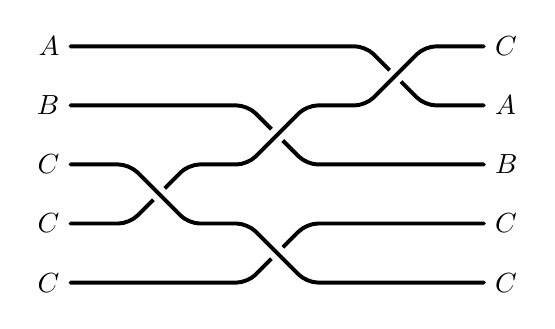
\begin{tikzpicture}
    \draw[line width=0.5mm, cap=round, rounded corners] (0,3) -- node[pos=0, left] {$A$} (3.75,3) -- (4.5,2.25) -- (5.25,2.25) node[pos=1, right] {$A$}; %% 5
    \draw[line width=0.5mm, cap=round, rounded corners] (0,2.25) -- node[pos=0, left] {$B$} (2.25,2.25) -- (3,1.5) -- (5.25,1.5) node[pos=1, right] {$B$}; %% 4
    \draw[line width=2mm, cap=round, rounded corners, color=white] (0,.75) -- (.75,.75) -- (1.5,1.5) -- (2.25,1.5) -- (3,2.25) -- (3.75,2.25) -- (4.5,3) -- (5.25,3) ; %% Shadow 2
    \draw[line width=0.5mm, cap=round, rounded corners] (0,.75) -- node[pos=0, left] {$C$} (.75,.75) -- (1.5,1.5) -- (2.25,1.5) -- (3,2.25) -- (3.75,2.25) -- (4.5,3) -- (5.25,3) node[pos=1, right] {$C$}; %% 2
    \draw[line width=0.5mm, cap=round, rounded corners] (0,0) -- node[pos=0, left] {$C$} (2.25,0) -- (3,.75) -- (5.25,.75) node[pos=1, right] {$C$}; %% 1
    \draw[line width=2mm, cap=round, rounded corners, color=white] (0,1.5) -- (.75,1.5) -- (1.5,.75) -- (2.25,.75) -- (3,0) -- (5.25,0); %% Shadow 3
    \draw[line width=0.5mm, cap=round, rounded corners] (0,1.5) -- node[pos=0, left] {$C$} (.75,1.5) -- (1.5,.75) -- (2.25,.75) -- (3,0) -- (5.25,0) node[pos=1, right] {$C$}; %% 3
    \end{tikzpicture}
    \]
    completely describes a map $A\otimes B\otimes C\otimes C\otimes C\rightarrow C\otimes A\otimes B\otimes C\otimes C$. If $\gamma$ is a symmetry, then only the permutation of the objects matters, hence the following braids induce the same morphism.
    \[
    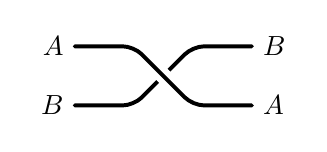
\begin{tikzpicture}
    \draw[line width=0.5mm, cap=round, rounded corners] (0,0) -- node[pos=0, left] {$B$} (.75,0) -- (1.5,.75) -- (2.25,.75) node[pos=1, right] {$B$}; %% 2
    \draw[line width=2mm, cap=round, rounded corners, color=white] (0,.75) -- node[pos=0, left] {$A$} (.75,.75) -- (1.5,0) -- (2.25,0) node[pos=1, right] {$A$}; %% shadow 1
    \draw[line width=0.5mm, cap=round, rounded corners] (0,.75) -- node[pos=0, left] {$A$} (.75,.75) -- (1.5,0) -- (2.25,0) node[pos=1, right] {$A$}; %% 1
    \end{tikzpicture}
    \quad
    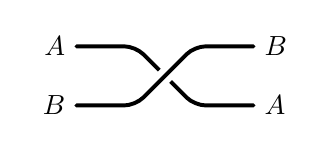
\begin{tikzpicture}
    \draw[line width=0.5mm, cap=round, rounded corners] (0,.75) -- node[pos=0, left] {$A$} (.75,.75) -- (1.5,0) -- (2.25,0) node[pos=1, right] {$A$}; %% 1
    \draw[line width=2mm, cap=round, rounded corners, color=white] (0,0) -- node[pos=0, left] {$B$} (.75,0) -- (1.5,.75) -- (2.25,.75) node[pos=1, right] {$B$}; %% 2
    \draw[line width=0.5mm, cap=round, rounded corners] (0,0) -- node[pos=0, left] {$B$} (.75,0) -- (1.5,.75) -- (2.25,.75) node[pos=1, right] {$B$}; %% 2
    \end{tikzpicture}
    \]
\end{rmk}

\begin{defn}
    Let $\cV$ and $\cW$ be braided monoidal categories, $F\colon\cV\rightarrow\cW$ a lax/strong/strict monoidal functor. We call $F$ a \emph{braided lax/strong/strict monoidal functor} if the diagram
    \[
    \begin{tikzcd}
        FA\otimes_\cW FB\ar[r, "\gamma_\cW"]\ar[d, "\phi"]
        & FB\otimes_\cW FA\ar[d, "\phi"] \\
        F(A\otimes_\cV B)\ar[r, "F\gamma_\cV"]
        & F(B\otimes_\cV A)
    \end{tikzcd}
    \]
    commutes.
    
    A \emph{braided natural transformation} is just a monoidal natural transformation between braided monoidal functors.
    
    If $\cV$ and $\cW$ are braided symmetric monoidal categories, then the braided functors and natural transformations are also called symmetric.
\end{defn}

\begin{exmp}
\item[(i)] If $\phi\colon R\rightarrow S$ is a map of commutative rings, then $S\otimes_R-\colon\Mod_R\rightarrow\Mod_S$ is a symmetric strong monoidal functor.

\item[(ii)] If $A$ is an abelian group, $(h,c)$ a normalized abelian 3-cocycle on $A$ with values in $R^\times$ and $\phi\colon R\rightarrow S$ a ring homomorphism, we have that $S\otimes_R-\colon A\text{-}\Mod_R^{(h,c)}\rightarrow A\text{-}\Mod_S^{(\phi h,\phi c)}$ is a braided strong monoidal functor. In particular, base change is a symmetric strong monoidal functor for both the trivial and the Koszul symmetry on $\bbZ\text{-}\Mod_R$.

\item[(iii)] If $F$ is a braided strong monoidal left adjoint, then the right adjoint is braided lax monoidal.
\end{exmp}

\begin{defn}
    Let $\cV$ be a braided monoidal category. A monoid $(M,\mu,\eta)$ in $\cV$ is \emph{commutative} if
    \[
    \begin{tikzcd}[column sep=tiny]
        M\otimes M\ar[rr, "\gamma_{M,M}"]\ar[dr, swap, "\mu"]
        && M\otimes M\ar[dl, "\mu"] \\
        & M
    \end{tikzcd}
    \]
    commutes.
    
    A \emph{morphism of commutative monoids} is just a morphism of monoids.
\end{defn}

\begin{rmk}
    In general, a lax monoidal functor will not lift to commutative monoids, but a braided lax monoidal functor will. It follows that we have a 2-functor $\CMon\colon\textbf{BrMonCAT}\rightarrow\CAT$, $\cV\mapsto\CMon(\cV)$, sending braided monoidal categories to their categories of commutative monoids.
\end{rmk}

\begin{thm}
    If $\cV$ is a locally presentable monoidal category with $-\otimes -$ cocontinuous in both variables, then $\CMon(\cV)\rightarrow\cV$ is monadic and accessible. Also, $\CMon(\cV)$ is locally $\kappa$-presentable if $\cV$ is.
\end{thm}

\begin{proof}
    Adapt the one for all monoids with an additional action.
\end{proof}

\begin{defn}
    Let $ \cV $ be a braided monoidal category.
    Define the \emph{opposite} of a $ \cV $-category~$ \cA $ by:
    \begin{enumerate}[label=$\bullet$]
	\item $ \Ob(\cA^{\op}) = \Ob(\cA) $,
	\item $ \cA^{\op}(A,B) = \cA(B,A) $,
	\item $ \id_A $ the same morphism as for $ \cA $ and
	\item composition by the diagram
	    \begin{displaymath}
	        \begin{tikzcd}
		    \cA^{\op}(B,C)\otimes \cA^{\op}(A,B)\arrow[r, equal] \arrow[d, dashed, "\circ_{\cA^{\op}}"]& \cA(C,B)\otimes \cA(B,A) \arrow[d, "\gamma"] \\
		    \cA^{\op}(A,C) = \cA(C,A) & \cA(B,A)\otimes \cA(C,B) \arrow[l, "\circ_\cA"]
	        \end{tikzcd}
	    \end{displaymath}
    \end{enumerate}
\end{defn}
We want to talk about $ \cV $-functors of ``several variables.''
For this we need $ \cA \otimes \cB$.
\begin{defn}
    Let $ \cA,\cB $ be $ \cV $-categories.
    Define the $ \cV $-category $ \cA \otimes \cB $ by
    \begin{enumerate}[label=$ \bullet $]
	\item $ \Ob(\cA\otimes \cB) = \Ob(\cA) \times \Ob(\cB) $
	\item $ (\cA\otimes\cB)((A,B),(A',B')) = \cA(A,A')\otimes \cB(B,B') $
	\item identities: $ I \iso I\otimes I \xrightarrow{\id_A \otimes \id_B} \cA\otimes\cB((A,B),(A,B)) $ and
	\item compositions
	    \begin{displaymath}
	        \begin{tikzcd}
		    (\cA(A',A'') \otimes \cB(B',B'')) \otimes (\cA(A,A') \otimes \cB(B,B'))
		    \arrow[d, "\text{isomorphism built from $ \gamma $'s}"]
		    \\
		    \cA(A',A'') \otimes \cA(A,A')\otimes \cB(B',B'')\otimes \cB(B,B')
		    \arrow[d, "\circ\otimes\circ"]\\
		    \cA(A,A'')\otimes \cB(B,B'')
	        \end{tikzcd}
	    \end{displaymath}
    \end{enumerate}
    Note: The first isomoprhism is unique, if $ \cV $ is symmetric.
\end{defn}
The final ingredient for Yoneda is enrichment of $ \cV $ over itself.
For this we need an internal $ \Hom $-functor.

\begin{defn}
    A monoidal category $ \cV $ is \emph{closed monoidal} if for any $ X \in \cV $ the functors $ X\otimes - $ and $ -\otimes X $ have right adjoints $ [X,-]_l $ and $ [-,X]_r $.
    We denote the unit and counit by $ \coev $ and $ \ev $ respectively.
    For example
    \begin{displaymath}
	\ev^X_Y \from [X,Y]_r \otimes X \rightarrow Y.
    \end{displaymath}
\end{defn}
\begin{rmk}
    If $ \cV $ is braided, we have $ -\otimes X \iso X\otimes - $, so $ [-,-]_l $ exists if and only $ [-,-]_r $ does and they are isomorphic.
    We simply write $ [-,-] = [-,-]_r $ in this case.
    In other words $ \cV(X\otimes Y,Z)\iso \cV(X,[Y,Z]) $.
\end{rmk}

\begin{rmk}
    If $ -\otimes X $ and $ X\otimes - $ have right adjoints, the monoidal natural transformatons may \emph{not} define a braiding $ \gamma $!
    We need more compatibility.
\end{rmk}

\begin{prop}
    Let $ \cV $ be a right-closed (that is $ [-,-]_r $ exists) monoidal category.
    Then the morphisms
    \begin{displaymath}
	([Y,Z]_r \otimes [X,Y]_r ) \to [X,Z]_r \quad \text{and} \quad I \to [X,X]_r
    \end{displaymath}
    correponding to
    \begin{displaymath}
	\begin{tikzcd}
	([Y,Z]_r \otimes [X,Y]_r) \otimes X \arrow[r]\arrow[d, "\alpha"'] & Z \\
	\lbrack Y,Z\rbrack_r \otimes ([X,Y]_r \otimes X) \arrow[r, "\id\otimes \ev^X"]  & \lbrack Y,Z\rbrack_r\otimes Y \arrow[u, "\ev^Y"']
    \end{tikzcd}\quad \text{and}\quad
    I\otimes X \xrightarrow{\lambda_X} X
    \end{displaymath}
    give a $ \cV $-category structure on $ \Ob(\cV) $ with undelying category isomorphic to $ \cV $.
\end{prop}
\begin{proof}
    The proof is slightly tedious; We refer to Kelly's book.

    A more abstract argument is possible if $ \cV $ is locally presentable and biclosed.
    The we have a monoidal left adjoint
    \begin{displaymath}
	\begin{tikzcd}[row sep = tiny]
	    \cV
	    \arrow[r, shift left=.5em] \arrow[from=r, shift left=.5em] \arrow[r,phantom, "\top"]
	    & \lbrack \cV,\cV\rbrack_{\kappa}
	    \arrow[r, shift left=.5em]
	    \arrow[from=r, shift left=.5em]
	    \arrow[r,phantom, "\top"]
	    & \lbrack \cV ,\cV \rbrack\\
	    X \arrow[mapsto, r] & -\otimes X
        \end{tikzcd}
    \end{displaymath}
    Use the $ [\cV,\cV] $-enrichment on $ \Ob(\cV) $ given by $ \langle\cV,\cW\rangle $ (previous exercise).
    Pull this back along the right adjoint and get $ R\langle \cV,\cW\rangle = [V,W]_r $.
\end{proof}

\begin{exmp}
    \begin{enumerate}[label=\arabic*)]
	\item 
	   If $ \cV $ is a category of ``sets with structure,'' that is if $ V \from \cV \to \Set $ is monadic for example $ \cV = \Mod_R,\Ab $ or $ \cV = \Top_{\mathrm{CGWH}} $, then $ [-,-] $ is just the obvious structure on $ \Hom $-sets of $ \cV $.
	   Specifically if $ M,N $ are $ R $-modules, then $ \Hom_R(M,N) $ has the natural $ R $-modules structure.
       \item
	   For $ \cV = \Cat $, $ [A,B] $ is just the category of functors from $ A $ to $ B $. Note that this is not just structure on the $ \Hom $-sets, we nned the additional data of natural transformations.
       \item Even more involved: $ \dgMod_R$, $\sSet $: 
    \end{enumerate}
\end{exmp}
If we have all these structures, that is a symmetric monoidal closed category, we can define a $ \cV $-functor
\begin{displaymath}
    \cC(-,-) \from \cC^{\op}\otimes \cC \to \cV
\end{displaymath}
as follows.
In order to do this, we use the following way of constructing functors $ \cA\otimes \cB \to \cC $:
\begin{prop}
    To give a $ \cV $-functor $ T\from \cA \otimes \cB \to \cC $ amounts to ginving families of functors $ T(A,-)\from \cB \to \cC)_{A \in \cA} $ and $ (T(-,B) \from \cA \to \cC)_{B\in \cB} $ such that
    \begin{enumerate}[label=\roman*)]
	\item
	    On objects $ T(A,-)(B) = T(-,B)(A) $ which we denote by $ T(A,B) $.
	\item 
	    For all $ A,A' \in \cA $ and $ B,B' \in \cB $ the diagram
	    \begin{displaymath}
		\begin{tikzcd}%[column sep = 3em]
		    \cA(A,A')\otimes \cB(B,B')
		    \arrow[r, "{T(-,B')\otimes T(A,-)}", bend left=18]
		    \arrow[dd, "\gamma"]
		    &
		    \cC(T(A,B') ,T(A',B')) \otimes \cC(T(A,B) ,T(A,B'))
		    \arrow[d, "\circ"]
		    \\
		    & \cC(T(A,B),T(A',B'))
		    \\
		    \cB(B,B') \otimes \cA(A,A') 
		    \arrow[r, "{T(A',-)\otimes T(-,B)}"', bend right=18]
		    & \cC(T(A',B) ,T(A',B')) \otimes \cC(T(A,B) ,T(A',B))
		    \arrow[u, "\circ"']
	        \end{tikzcd}
	    \end{displaymath}
	    commutes.
	    This means that ``it does not matter in which way we compose.''
	    In this case, $ T_{(A,B),(A',B')}  $ is given by the now well defined composite in the above diagram.
    \end{enumerate}
\end{prop}
\begin{proof}
    Long exercise.
\end{proof}
Now we need to define $ \cC(c,-) \from \cC \to \cV $, $ \cC(-,c)\from \cC^{\op}\to \cV $.
But $ \cC(-,c) $ is just $ \cC^{\op}(c,-) $, so we only need to prove that the covariant one is a well defined functor.
On objects we define $ \cC(c,-)(c') = \cC(c,c') \in \cV $.
The action on morphisms is given by the morphism
\begin{displaymath}
    \cC(c,-)_{c',c''} \from \cC(c',c'') \to [\cC(c,c'),\cC(c',c'')]
\end{displaymath}
corrseponding under adjunction to the composition
\begin{displaymath}
    \cC(c',c'')\otimes \cC(c,c') \xrightarrow{\circ} \cC(c,c'')
\end{displaymath}
The diagram in the above proposition commutes by adjunction since composition is associative.
\begin{exmp}
    \begin{enumerate}[label=\arabic*)]
	\item
	    For $ \cV =  $``sets with structure,'' the functor $ \cC(-,-) $ simply defines a lift 
	    \begin{displaymath}
	        \begin{tikzcd}
	    	& \cV \arrow[dd, "V"]\\
	    	\cC^{\op}\otimes \cC \arrow[ur, "{\cC(-,-)}"]\arrow[dr, "{\cC_0(-,-)}"'] & \\
	    	& \Set
	        \end{tikzcd}
	    \end{displaymath}
	    we remember that $ \cC(-,-) $ is an $ R $-module, a topological space, etc.
	\item
	    For $ \cC = \Cat $, we get $ \cK(-,-) \from \cK^{\op}\times \cK \to \Cat $, $ (x,y)\mapsto \cK(x,y) $.
	    a 2-functor, where the action on 1-cells is given by whiskering on either side.
	\item
	    For $ \cV $ itself, we get  $ \cV(-,-) \from \cV^{\op}\otimes \cV \to \cV $, $ (V,W)\mapsto [V,W] $.
	    The underlying set of this is $ \cV(I,[V,W]) \iso \cV(V,W) $.
	    To avoid confusion, we will write $ \cV_0(V,W) $ for the \emph{set} of morphisms in $ \cV $.
    \end{enumerate}
    %What about using $ \underline{\cV} $ for enriched sets?
    %If we do this add a shortcut.
\end{exmp}
\begin{prop}
    Ther is a $ \cV $-functor $ -\otimes -\from \cV \otimes \cV \to \cV $ which on $ \Hom $-objects is the morphism
    \begin{displaymath}
        [X,X']\otimes [Y,Y'] \to [X\otimes Y , X'\otimes Y']
    \end{displaymath}
    corresponding by adjunction to the morphism
    \begin{displaymath}
        ([X,X']\otimes[Y,Y']) \otimes (X\otimes Y)\iso ([X,X']\otimes X)\otimes ([Y,Y']\otimes Y) \xrightarrow{\ev^X \otimes \ev^Y} X'\otimes Y'.
    \end{displaymath}
    For this functor, $ \alpha,\lambda,\rho $ are $ \cV $-natural transformations. Moreover for each $ X $, the maps $ \ev^X $ and $ \coev^X $ are $ \cV $-natural, so $ -\otimes X $ is a left adjoint to the functor $ [X,-] $ in $ \cV $-$\CAT$
\end{prop}
\begin{proof}
    By adjunction. Straightforward, but tedious (see Kelly).
\end{proof}
\begin{rmk}
    One can check that all ``reasonable'' morphisms built from the canonical ones are $ \cV $-natural.
    For example, if $ f \from A \to B $ is a morphism in $ \cA_0 $, we get $ \cV $-natural transformations 
    \begin{displaymath}
        \cA(f,-) \from \cA(B,-)\Rightarrow \cA(A,-) \quad \text{and} \quad  \cA(-,f) \from \cA(-,A) \Rightarrow \cA(-,B) 
    \end{displaymath}defined by applying
    \begin{displaymath}
        \cA_0^{\op}\times \cA_0 \to (\cA^{\op} \otimes \cA) \xrightarrow{\cA(-,-)_0} \cV_0
    \end{displaymath}
    to $ (f,\id) $ and $ (\id,f) $ respectively.
    
    Further details---or more precisely---a good list of instructions on how to preceed efficiently can be found in \cite[\S 1.7 and 1.8]{Kelly}.
\end{rmk}


\section{The weak Yoneda Lemma}

\begin{rmk}
    With the morphism just defined, we can sxporess $ \cV $-naturality of $ \alpha \from F \Rightarrow G $ where $ F,G\from \cC \to \cD $ by saying that the following diagram commutes for all $ c,c' \in \cC $:
    \begin{displaymath}
	\begin{tikzcd}[column sep = huge]
	    \cC(c,c') \arrow[r, "F"]\arrow[d, "G"]& \cD(Fc, Fc')\arrow[d, "{\cD(Fc,\alpha_{c'})}"] \\
	    \cD(Gc,Gc') \arrow[r, "{\cD(\alpha_c, Gc')}"' ]& \cD(Fc,Gc')
        \end{tikzcd}
    \end{displaymath}
\end{rmk}

\begin{thm}[Weak Yoneda lemma]
    Let $\cV$ be a symmetric monoidal category, $\cA$ a $\cV$-category, $F\colon\cA\rightarrow\cV$ a $\cV$-functor, $A\in\cA$ and $\alpha\colon\cA(A,-)\Rightarrow F$ a $\cV$-natural transformation. Consider the map$$\phi(A)\colon I\xrightarrow{\id_A}\cA(A,-)\xrightarrow{\alpha_A}FA.$$
    The assignment
    \begin{align*}
        \phi\colon\cV\text{-}\Nat(\cA(A,-),F) &\rightarrow\cV_0(I,FA) \\
        A &\mapsto\phi(A)
    \end{align*}
    is a bijection, where the inserve map $\psi$ is given by sending $\eta\colon I\rightarrow FA$ to the $\cV$-natural transformation
    $$\cA(A,B)\xRightarrow{F_{A,B}}[FA,FB]\xRightarrow{[\eta,\id_{FA}]}[I,FA]\cong FA.$$
\end{thm}

\begin{proof}
    $\cV$-naturality follows from the general principle previously mentioned that ``all'' morphisms coming from the monoidal structure are $\cV$-natural. Since $F_{A,A}(\id_A)=\id_{FA}$, we get $\phi\psi=\id$ by construction. We still have to prove that $\psi\phi=\id$.
    
    Consider the diagram
    \[
    \begin{tikzcd}
        \cA(A,B)\ar[r, "{\cA(A,-)}"]\ar[d, "F"]
        & {[\cA(A,A),\cA(A,B)]}\ar[r, "{[\id_A,I]}"]\ar[d, "{[I,\alpha_B]}"]
        & {[I,\cA(A,B)]}\ar[r, "\sim"]\ar[d, "{[I,\alpha_B]}"]
        & \cA(A,B)\ar[d, "\alpha_B"] \\
        {[FA,FB]}\ar[r, "{[\alpha_A,I]}"]\ar[rrr, bend right, dotted, "{[\phi(B),I]}"]
        & {[\cA(A,A),FA]}\ar[r, "{[\id_A,I]}"]
        & {[I,FB]}\ar[r, "\sim"]
        & FA
    \end{tikzcd}
    ,\]
    where the left and right squares on extremes commute by $\cV$-naturality, while for the one in the middle we consider the functor $[-,-]\colon\cV^{\op}\otimes\cV\rightarrow\cV$.
    
    The claim follows by checking that the composition is the identity.
\end{proof}

\begin{thm}[Parametrized Yoneda]
    Let $T\colon\cB^{\op}\otimes\cA\rightarrow\cV$ be a $\cV$-functor and suppose that for all $B\in\cB$ there exists a $KB\in\cA$ and a $\cV$-natural isomorphism $\alpha_B\colon\cA(KB,-)\xRightarrow{\sim} T(B,-)$. Then there is a unique way to define $K_{B,C}\colon\cB(B,C)\rightarrow\cA(KB,KC)$ in $\cV$ such that $K$ is a $\cV$-functor and $(\alpha_B)_A\colon\cA(KB,A)\rightarrow T(B,A)$ is $\cV$-natural in both variables as a $\cV$-functor $\cB^{\op}\otimes\cA\rightarrow\cV$.
\end{thm}

\begin{proof}
    One checks that $\cV$-naturality of $(\alpha_A)_B$ amounts to commutativity of the diagram
    \[
    \begin{tikzcd}[column sep = 5em]
        \cB(B,C)\ar[r, dotted, "K_{B,C}"]\ar[d, "{T(-,KC)}"]
        & \cA(KB,KC)\ar[r, "{T(B,-)}"]\ar[dr, "\sim"', swap, "{(\alpha_B)_{KC}}"]
        & {[T(B,KB),T(B,KC)]}\ar[d, "{[\eta_B, I]}"] \\
        {[T(C,KC),T(B,KC)]}\ar[rr, "{[\eta_C,I]}"]
        && {[I,T(B,KC)]}
    \end{tikzcd}
    ,\]
    where $\eta_B=\phi(\alpha_B)$ and the triangle commutes by Yoneda. Since $(\alpha_B)_{KC}$ is an isomorphism there exists a unique candidate $K_{B,C}$ and one only has to check that it works.
\end{proof}

\begin{rmk}
    This is really useful as a way of constructing $\cV$-functors via universal properties and representability results.
\end{rmk}

\section{Weighted colimits and enriched presheaf categories}

We want to define the $\cV$-category $[\cA^{\op},\cV]$ of $\cV$-presheaves or $\cV$-functors for $\cA$ small. We will do this by defining a suitable $\cV$-monad $T$ such that $[\cA^{\op},\cV]\coloneqq T\Alg$. We want our category to have at least coproducts and equalizers, so from now on we assume that $\cV$ is a (co)complete, symmetric monoidal and closed. Such an object is called \emph{cosmos}, after \emph{B\'enabou cosmos}.

\begin{defn}
    Let $\cC$ be a $\cV$-category, $(C_j)_{j\in J}\in\Ob(\cC)^J$ a family of objects in $\cC$. We say that a collection $j_j\colon C_j\rightarrow C$ exhibits $C$ as a $\cV$-coproduct of the $(C_j)_{j\in J}$ if$$\cC(j_j,D)\colon\cC(C,D)\rightarrow\cC(C_j,D)$$is a product diagram in $\cV_0$ for all $D\in\cC$.
    
    Similarly, we define a $\cV$-coequalizer$$A\rightrightarrows B\rightarrow C$$ by requiring that $$\cC(C,D)\rightarrow\cC(B,D)\rightrightarrows\cC(A,D)$$is a coequalizer in $\cV_0$.
    
    Dualizing the definitions, we find the notions of \emph{product} and \emph{equalizer}.
\end{defn}

\begin{rmk}
    If we apply $\cV_0(A,-)\colon\cV_0\rightarrow\Set$, we see that $\cV$-coproducts and $\cV$-coequalizers are in particular coproducts and coequalizers in $\cV_0$.
\end{rmk}

\begin{exmp}
    For $\cV=\Cat$, a $\cV$-coequalizer also has a 2-dimensional universal property, that is given one $A\rightrightarrows B\rightarrow C$ and a 2-cell from $B$ to $D$ there is a unique 2-cell from $C$ to $D$ making the following diagram commute.
    \[
    \begin{tikzcd}
    	&& C\ar[dd, dotted, swap, "\bar{b}", ""{name=bbar}]\ar[dd, dotted, bend left=60, "\bar{a}", ""{name=abar}] \\
        A\ar[r, shift left,]\ar[r, shift right]
        & B\ar[ur]\ar[dr, "a", ""{name=a}]\ar[dr, bend right=60, swap, "b", ""{name=b}] \\
        && D
        \ar[Rightarrow, shorten <= .3em, shorten >= .3em, from=a, to=b, "\alpha"]
        \ar[Rightarrow, dotted, shorten <= .3em, shorten >= .3em, swap, from=abar, to=bbar, "\overline{\alpha}"]
    \end{tikzcd}
    \]
\end{exmp}

For enriched categories, there is an important third kind of colimit called \emph{copower} or \emph{tensor}.

\begin{defn}
    Let $\cC$ be a $\cV$-category, $V\in\cV$, $C\in\cC$. We say that the copower of $C$ by $V$ exists if the $\cV$-functor $[V,\cC(C,-)]\colon\cC\rightarrow\cV$ is representable by some object $V\odot C\in\cC$, the copower, that is we have a $\cV$-natural isomorphism $\cC(V\odot C,-)\xRightarrow{\sim}[V,\cC(C,-)]$.
    
    Dualizing the definition, we find the notion of \emph{power} or \emph{cotensor}.
\end{defn}

\begin{rmk}
    By parametrized Yoneda, we get a $\cV$-functor$$-\odot-\colon\cV\otimes\cC\rightarrow\cC$$if all copowers exist. It is associative up to coherent isomorphism, so it defines a kind of weak action of $\cV$ on $\cC$.
\end{rmk}

\begin{exmp}
    For $\cV=\cC=\Cat$, $C\times[1]$ is the copower of $C\in\cC$ by $[1]\in\cV$. Indeed, we have a pair of bijective correspondences inducing the one we want as follows:
    
    $$C\times[1]\rightarrow D\quad\leftrightarrow\quad
        \begin{tikzcd}
        C\ar[r, bend left, ""{name=A}]\ar[r, bend right, swap, ""{name=B}]
        & C
        \ar[Rightarrow, shorten <= .3em, shorten >= .3em, from=A, to=B, "\alpha"]
    \end{tikzcd}
    \quad\leftrightarrow\quad C\rightarrow D^{[1]}.$$
\end{exmp}

\begin{prop}
    A $\cV$-category $\cC$ has $\cV$-coproducts and $\cV$-coequalizers if $\cC_0$ has coproducts and coequalizers and these are preserved by the functor $\cC_0(-,D)\colon\cC_0\rightarrow\cV^{\op}$ for every $D\in\cC$.
\end{prop}

\begin{proof}
    It follows from the definition.
\end{proof}

\begin{cor}
    The $\cV$-categories $\cV$ and $\cV^{\op}$ have all $\cV$-coproducts and $\cV$-coequalizers.
\end{cor}

\begin{proof}
    We need to check that $[-,V]_0\colon\cC_0\rightarrow\cV_0^{\op}$ preserves coproducts and coequalizers, but this is just $[-,V]\colon\cV_0\rightarrow\cV_0^{\op}$ and we have $[-,V]\dashv[-,V]\colon\cV_0^{\op}\rightarrow\cV_0$ because
    $$\cV_0(X,[Y,Z])\cong\cV_0(X\otimes Y,Z)\cong\cV_0(Y\otimes X,Z)\cong\cV_0(Y,[X,Z]).$$
    
    For $\cV^{\op}$, we need to check that $[V,-]_0\colon\cV_0\rightarrow\cV_0^{\op}$ preserves the limits, which follows from $-\otimes V\dashv [V,-]$.
\end{proof}

\begin{prop}
    The $\cV$-category $\cV$ has all powers and copowers given by $[V,C]$ and $V\otimes C$ respectively.
\end{prop}

\begin{proof}
    We need $\cV$-natural isomorphisms $[V,[C,D]]\cong[V\otimes C,D]$, which follows from the fact that we have a $\cV$-adjunction $-\otimes C\dashv [C,-]$. Similarly, use the symmetry isomorphism to get a $\cV$-natural isomorphism $[D,[V,C]]\cong[V,[D,C]]$.
\end{proof}

\begin{defn}
    A $\cV$-category $\cC$ is \emph{$\cV$-cocomplete} if it has all $\cV$-coequalizers, $\cV$-coproducts and copowers. If it satisfies the dual conditions, then it is \emph{$\cV$-complete}.
\end{defn}

\begin{exmp}
    If $(\cC_j)_{j\in J}$ is a family of $\cV$-(co)complete $\cV$-categories, then $\Pi_{j\in J}\cC_j$ is a $\cV$-(co)complete $\cV$-category.
\end{exmp}

\begin{prop}
   If $\C$ has powers (cotensors), then $\C$ is cocomplete, if and only if $\C_{0}$ is cocomplete and $\C$ has copowers.
\end{prop}

\begin{proof}
   $"\Rightarrow ":$ We have already seen this. \\
   $"\Leftarrow ":$ We need to show, that ordinary coequalizers and coproducts in $\C_{0}$ are automatically $\V$-coequalizers and $\V$-coproducts. 
   We will just check the case of coequalizers and leave the other case for the reader. We know, that we have a natural bijection of sets between 
   equalizers 
      \begin{center}
         \begin{tikzcd}
            \C_{0}(K,D) \arrow[r, "\iso"] & \Eq(\C_{0}(B,D) \arrow[r, shift left, "f^{\ast}"] \arrow[r, shift right, "g^{\ast}"'] & \C_{0}(A,D))
         \end{tikzcd}
      \end{center}
   and coequalizers 
      \begin{center}
         \begin{tikzcd}
            A \arrow[r, shift left, "f"] \arrow[r, shift right, "g"'] & B \arrow[r, "k"] & K
         \end{tikzcd}
      \end{center}
   in $\C_{0}$. For each $E \in \C$ and $V \in \V_{0}$, we thus have 
      \begin{center}
         \begin{tikzcd}
             \C_{0}(K.E^{V}) \arrow[r] \arrow[d, "\iso"'] & \C_{0}(B,E^{V}) \arrow[r, shift left] \arrow[r, shift right] \arrow[d, "\iso"] & \C_{0}(A,E^{V}) \arrow[d, "\iso"] \\
             \V_{0}(V,\C(K,E)) \arrow[r] & \V_{0}(V,\C(B,E)) \arrow[r, shift left] \arrow[r, shift right] & \V_{0}(V,\C(A,E))
         \end{tikzcd}
      \end{center}
   and since this holds for all $V \in \V_{0}$, this implies that $\C(K,E) \iso \Eq(f^{\ast},g^{\ast})$ in $\V$, as claimed.
\end{proof}

\begin{cor}
   $\V$ is complete and cocomplete as $\V$-category.
\end{cor}

\begin{rmk}
   Note, that the existence of powers for a strong generating set suffices. 
\end{rmk}

\begin{defn}
   We say, that a $\V$-functor $F \from \C \to \D$ preserves (certain) $\V$-coequalizers or $\V$-coproducts, if $F_{0} \from \C_{0} \to \D_{0}$ preserves
   coequalizers or coproducts. $[V]$
\end{defn}

To talk about preservation of copowers, we need a canonical comparison morphism $\bar{F} \from V\copw FC \to F(V\copw C)$, which we define to be 
   \begin{center}
      \begin{tikzcd}
         I \arrow[r] \arrow[d, "\eta"'] & \D (V \copw FC,F(V\copw C)) \\
         \lbrack V,\C (C,V \copw C)\rbrack \arrow[r] 
         & \lbrack V,\D (FC,F(V\copw C))\rbrack \arrow[u, "\iso"']
      \end{tikzcd}
   \end{center}
where the lower horizontal morphism is $[V,F]$ and $\eta$ corresponds via weak Yoneda to the $\V$-natural isomorphism $\C(V\copw C,\_) \iso [V,\C(C,\_)]$.

\begin{defn}
   We say, that $F$ preserves the copower $V \copw C$ if $\bar{F} \from V \copw FC \to F(V \copw C)$ is an isomorphism in $\D_{0}$.
\end{defn}

\begin{lemma}
   Let $\C$ be a $\V$-category and $\B \subset \C$ the full subcategory, generated by those object $B \in \C$ such that $V \copw B$ exists (in $\C$) for all
   $V \in \V$. Then $\B$ is closed in $\C$ under $\V$-coequalizers and $\V$-coproducts.
\end{lemma}

\begin{proof}
    Let 
       \begin{center}
          \begin{tikzcd}
              A \arrow[r, shift left, "f"] \arrow[r, shift right, "g"'] & B \arrow[r, "k"] & K
          \end{tikzcd}
       \end{center}
    be a $\V$-coequalizer, such that $B,A \in \B$. We need to show, that the $\V$-coequalizer of 
       \begin{center}
          \begin{tikzcd}
             V \copw A \arrow[r, shift left, "V\copw f"] \arrow[r, shift right, "V\copw g"'] & V \copw B
          \end{tikzcd}
       \end{center}
    is given by $V \copw K$. Indeed we have an induced isomorphism
       \begin{center}
          \begin{tikzcd}
             \C(V \copw K,D) \arrow[r, "eq"] \arrow[d, dashed, "\exists !", "\iso"'] & \C(V\copw,D) \arrow[r, shift left] \arrow[r, shift right] \arrow[d, "\iso"] & 
                \C(V \copw A, D) \arrow[d, "\iso"] \\
             \lbrack V,\C(K,D) \rbrack \arrow[r, "eq"'] & \lbrack V,\C(B,D) \rbrack \arrow[r, shift left] \arrow[r, shift right] & \lbrack V,\C(A,D) \rbrack 
          \end{tikzcd}
       \end{center}
    and the proof for coproducts is similar. 
\end{proof}

\begin{thm}
   Let $\C$ be a complete $\V$-category and let $T \from \C \to \C$ be a $\V$-monad. Then $T\Alg$ is complete and $U \from T\Alg \to \C$ preserves $\cV$-powers, 
   $\V$-products and $\V$-equalizers. If $\C$ is also cocomplete, then $T\Alg$ is cocomplete, if and only if the underlying unenriched category 
   $(T\Alg)_{0} \iso T_{0}\Alg$ is cocomplete.
\end{thm}

\begin{proof}
   We know that $T_{0}\Alg$ is complete, so we need to show that equalizers and products are $\V$-equalizers and $\V$-products. But hom-objects are 
   defined as equalizers in $\V$
      \begin{center}
         \begin{tikzcd}
            T\Alg((A,a),(B,b)) \arrow[r] & \C(A,B) \arrow[r, shift left] \arrow[r, shift right] & \C(TA,B)
         \end{tikzcd}
      \end{center}
   and we thus get the claim for $\V$-equalizers and $\V$-products, since equalizers and products commute with equalizers in $\V_{0}$. We will leave the
   claim for powers as an exercise. But once we have the powers, we get from the cocompleteness of $T_{0}\Alg$, that $T\Alg$ has $\V$-coequalizers and
   $\V$-coproducts. So it remains to show, that $T\Alg$ has copowers. For this we use the lemma above. Since every object is a coequalizer of free 
   algebras, hence a $\V$-coequalizer, it suffices to check this for free algebras, i.e. algebras is the image of the left $\V$-adjoint 
   $F \from \C \to T\Alg$. So we are done if we can show, that left $\V$-adjoints preserve copowers. This follows from the next proposition. 
\end{proof}

\begin{prop}
   Left $\V$-adjoints preserve $\V$-coequalizers, $\V$-coproducts and copowers.
\end{prop}

\begin{proof}
   Let $F \from \C \to \D$ be a left $\V$-adjoint $U\vdash F$. The claims all follow as in the unenriched case. For copowers we have the isomorphisms
      \begin{align*}
         \D(F(V\copw C),D) \iso \C(V\copw C,UD) \iso \lbrack V,\C(C,UD) \rbrack \iso \lbrack V,\D(FC,D) \rbrack 
      \end{align*}
    and one checks, that this is the coup morphism it the target has copowers. 
\end{proof}

We are now ready to define enriched presheaf categories. Let $\A$ be a small $\V$-category. Then $\prod_{A \in \Ob(\A)}\V$ is clearly a complete and 
cocomplete $\V$-category with everything computed pointwise. We define the $\V$-monad for presheafs by 
   \begin{align*}
      T((FA)_{A \in \Ob(\A)}) = \left(\coprod_{A \in \Ob(\A)}\A(B,A)\copw FA\right)_{B \in \Ob(\A)}
   \end{align*} 
with unit given by identities and multiplication given by composition. A $T$-algebra is thus a collection $(FA) \in \prod_{A \in \Ob(\A)}\V$ with action 
$\coprod \A(B,A) \copw FA \to FB$, which amounts precisely to a $\V$-functor $\A(B,A) \to [FA,FB]$ i.e. a $\V$-functor $\A^{\op} \to \V$.

\begin{defn}
   We write $[\A^{\op},\V]$ for $T\Alg$ and call it the $\V$-category of $\V$-presheafs on $\A$. By construction we have 
   $[\A^{\op},\V]_{0} = \V$-$\CAT(\A^{op},\V)$.
\end{defn}

\begin{rmk}:
   \begin{itemize}
      \item[(1)]
         The same construction works for any cocomplete $\V$-category $\C$ and we get $\V$-categories $[\A^{\op},\C]$ and $[\A,\C]$.
      \item[(2)]
         The statement ``$T$ is a $\V$-monad'' actually needs to be checked. It can be done using Kelly (1.7,1.8)   % to ref
         and the universal properties of $\coprod$ and $\copw$ (see also later exercise).
      \item[(3)]
         We have as enriched Yoneda lemma basically by definition: Taking the free algebra of the collection $(I_{A})_{B \in \Ob(\A)}$, given by 
         $I$ if $B=A$ and $\emptyset$ else, is precisely $\A(\_,A)$. So we get isomorphisms 
            \begin{center}
               $\lbrack \A^{\op},\V \rbrack (\A(\_,A),F) \iso T\Alg((F(I_{A})),F) \iso \prod \V(I_{A},(FB)_{B\in \A}) \iso FA$
            \end{center}
      \item[(4)]
         The hom-object is by definition the equalizer
            \begin{center}
               \begin{tikzcd}
                  \lbrack \A^{\op},\V \rbrack (F,G) \arrow[r] & \prod_{A} \lbrack FA,GA \rbrack \arrow[r, shift left] \arrow[r, shift right] & 
                     \prod_{A,B} \lbrack \A(A,B) \copw FA,GB \rbrack
               \end{tikzcd}
            \end{center}
   \end{itemize}
\end{rmk}

\begin{prop}
   The $\V$-categories $[\A^{\op},\C]$ and $[\A,\C]$ are complete (resp. cocomplete), if $\A$ is small and $\C$ is complete (resp. cocomplete).
\end{prop}

\begin{proof}
   This follows, since $T_{0}$ is cocontinous. 
\end{proof}

\begin{defn}
   Given a $\V$-category $\C$ and a $\V$-functor $K \from \A \to \C$, where $\A$ is small, we have a natural $T$-action on the $\V$-functor 
   $\C \to \prod_{\Ob(\A)}\V$ given by the assignment $c \mapsto \C(Ka,c)$. Now we write 
      \begin{align*}
         \C(K,-) \from \C \to [\A^{\op},\V]
      \end{align*}
   for the induced $\V$-functor given by sending $c$ to $\C(K-,c)$. This is also written as $\widetilde{K}$.
\end{defn}

\begin{defn}
   Given a $\V$-presheaf $W\from \A^{\op} \to \V$ and a $\V$-functor $K \from \A \to \C$, we say that the $W$-weighted colimit of $K$ exists if 
      \begin{align*}
         [\A^{\op},\V](W,\cC(K,-))\colon\cC\rightarrow\Set
      \end{align*} 
   is corepresentable, that is there is a corepresenting object denoted by $W \copw_{\A} K$, such that
      \begin{align*}
         \C(W\copw_{\A} K, c) \iso [\A^{\op},\V](W,\C(K-,c))
      \end{align*}
      naturally in $c\in\cC$.
\end{defn}
  
We can think of $Wa\to\C(Ka,c)$ as a bunch of enriched cocones.
\begin{exmp}
    \begin{enumerate}[label=(\roman*)]
    \item If $\A=\J$ with $\Ob(\J)=*$ and $\J(*,*)=\{\id_*\}$, then $[\J^{\op},\V\}\cong\V$ and every $\J\to\C$ amounts to give an object $c\in\C$. Hence $v\copw_{\J} c$ is simply the copower $v\copw c$.
    \item If $\D$ is an unenriched small category, we can consider the free $\V$-category $(I)_*\D$. Then giving a $\V$-functor $(I)_*\D\to\C$ is the same as giving a functor $\D\to\C_0$. The conical weight $\Delta_{I}\from(I)_*\D^{\op}\to\V$ gives us a functor $\D^{\op}\to\V_0$ sending the whole category to the identity of the monoidal category $\V$. Then $\Delta_I\copw_{I_*D}F$ is really the same as a colimit of $\widetilde{F}\from \D\to\C_0$ with the additional property that $\C(\colim\widetilde{F}d, c)\cong \lim\C(Fd, c)$ in $\V$ (rather than just a bijection of sets).
    In particular, when $\C$ has powers there is no distinction between colimits in $\C_0$ and $\Delta_I$-weighted colimits. Powers make it possible to lift the bijection of sets to an isomorphism in $\V$ via (unenriched) Yoneda for $\V_0$. The $\Delta_I$-weighted colimits are called \emph{conical} colimits. In particular, $\V$-coequalizers and $\V$-coproducts are conical colimits.
    \end{enumerate}
\end{exmp}
\begin{thm}
   Let $\C$ be a $\V$-category. TFAE:
   \begin{enumerate}
       \item The $\V$-category $\C$ is cocomplete.
       \item For each small $\V$-category $\A$ and each $\V$-functor $K\from\A\to\C$, the functor $\Hom_{\A}(K,-)\from\C\to[\A^{\op},\V]$ has a left $\V$-adjoint $-\copw_{\A} K\from [\A^{\op},\V]\to\C$.
       \item The category $\C$ has all weighted colimits.
   \end{enumerate}
\end{thm}
\begin{proof}
In the example we saw $3\Rightarrow1$ and clearly $2\Rightarrow3$ by definition. It remains to show $1\Rightarrow2$. By the parametrized Yoneda lemma, we need to show that 
$$W\mapsto[\A^{\op},\V](W,\Hom_{\A}(K,-))$$
is representable for every $W\in[\A^{\op},\V]$. Every such $W$ is canonically a $\V$-coequalizer of free objects (recall that $[\A^{\op},\V]=T\Alg$). Let $\B\subseteq[\A^{\op},\V]$ be the subcategory of $W$ such that $[\A^{\op},\V](W,\Hom_{\A}(K,-))$ is representable. By assumption, $B$ is closed under copowers, $\V$-coproducts and $\V$-coequalizers. Thus it suffices to show that if $W$ is a free $T$-algebra, then $W\in\B$. Using copowers and coproducts, we can reduce the case $W=T(V_A)_{A\in\A}$ to $T(I_{\A})$ where 
$$(I_{\A})=\begin{cases} \emptyset, & \mbox{if } \B\ne\A \\ I, & \mbox{if } \B=\A
\end{cases}$$
Therefore $$(V_A)_{A\in\A}=\coprod{V_{\A}\copw I_{\A}}\in\prod_{A\in\A}\V$$
so that we are reduced to checking $T(I_{\A})\in\B$. But $T(I_{\A})=\A(-,A)$ by definition of $T$. Here we have 
$$[\A^{\op},\V](T(I_{\A}),\Hom_{\A}(K,-))\cong\prod\V(I_{\A},(\C(KB,-))_{B\in\A})\cong\C(KA,-)$$
so this is represented by $KA\in\C$.
\end{proof}
\begin{rmk}
   We may extract a formula from the proof above. Then we find $$\A(-,A)\copw_{\A}K=KA$$ and $$W\copw_{\A}K=\text{coeq}\left(\coprod_{A,B}(WB\otimes\A(A,B))\copw KA\rightrightarrows\coprod_{A}WA\otimes KA \right)$$
\end{rmk}
\begin{cor}
    For all small $\A$, $[\A,\V]$ has weighted colimits.
\end{cor}
\begin{exmp}
    Take $\V=\Cat$ and $\K$ a (cocomplete) $2$-category. In this case, $[\A,\K]$ us the $2$-category with $0$-cells the $2$-functors, $1$-cells the $2$-natural transformations and $2$-cells the so-called \emph{modifications}.
\end{exmp}
\begin{defn}
   Let $\alpha,\beta\colon F\Rightarrow G\colon\A\to\K$ be $2$-natural transformations. A modification $\varphi\from\alpha\Rrightarrow\beta$ is a collection of $2$-cells $(\varphi_A\colon\alpha_A\Rightarrow\beta_A)_{A\in\A}$ in $\K$, such that 
   \[
    \begin{minipage}{0.3\linewidth}
        \begin{tikzcd}[row sep=1cm, column sep=1cm]
           FA\arrow[d, "Ff"'] \arrow[r, bend right, "\beta_A"', ""{name=D, anchor=center}] \arrow[r, bend left,"\alpha_A", ""{name=U, anchor=center}] & GA \arrow[d, "Gf"] \\
 FB\arrow[r, "\beta_B"']            &GB      
      \ar[Rightarrow, shorten <= .3em, shorten >= .3em, "\varphi_A"', from=U, to=D]
 \end{tikzcd}
    \end{minipage}
    \hspace{-1.3cm}
            =
	\hspace{.4cm}
	\begin{minipage}{0.3\linewidth}
		\begin{tikzcd}[row sep=1cm, column sep=1cm]
 FA\arrow[d,"Ff"'] \arrow[r, "\alpha_A"]                        &  GA\arrow[d,"Gf"] \\
 FB\arrow[r, bend right, "\beta_B"', ""{name=D, anchor=center}] \arrow[r, bend left,"\alpha_B", ""{name=U, anchor=center}] &    GB    
 \ar[Rightarrow, shorten <= .3em, shorten >= .3em, "\varphi_B"', from=U, to=D]
		\end{tikzcd}
	\end{minipage}
    \]
   holds for every $f\from A\to B$
\end{defn}
Take $\A=\hspace{-1.5mm}\begin{tikzcd}[row sep=1cm, column sep=1.3cm]
		0\hspace{-1.5mm}\arrow[r, "f_1" description,  shift right=.5ex, shorten <= .3em, shorten >= .3em]  \arrow[r, "f_0", shift left=1ex, shorten <= .3em, shorten >= .3em] & \hspace{-1.5mm}1
		\end{tikzcd}\hspace{-1.5mm}$ and $W\from\A\to\Cat$ sending $0$ to the terminal category $*$, $1$ to the category $[1]=(0\to 1)$ and such that $Wf_i=\text{incl}_i\from *\to[1]$ are the inclusions of the domain and the target in the walking arrow. The $W$-weighted limit represents $[\A,\Cat](W,\C(c,F-))$ for $F\from\A\to\C$. This amounts to a morphism $c\xrightarrow{c}F_0$ and a $2$-cell 
		\[
		\begin{tikzcd}
	    & F_0\ar[dd, "\gamma", Rightarrow, shorten <= 1.8em, shorten >= 1.8em]\ar[dr, "Ff_0"]&\\
	    c\ar[dr,"c"]\ar[ur,"c"]&&F_1\\
	    &F_0\ar[ur,"Ff_1"']&
	\end{tikzcd}
\]
as objects, while morphisms are modifications. A priori, these are two natural transformations 
\[
\begin{tikzcd}[row sep=1cm, column sep=1cm]
         W_i^{\phantom{p}}\arrow[r, bend right, "{(d,\delta)}"', ""{name=D, anchor=center}] \arrow[r, bend left,"{(c,\gamma)}", ""{name=U, anchor=center}] & \hspace*{5mm}\C(c,F-) 
          \ar[Rightarrow, shorten <= .5em, shorten >= .5em, "\varphi_i"', from=U, to=D]
         \end{tikzcd}
         \]
but $\varphi_i$ is determined by $\varphi_0$, so we are left with a single equation.
\begin{center}
    \begin{minipage}{0.3\linewidth}
		\begin{tikzcd}[row sep=1cm, column sep=1cm]
		&  F_0\arrow[d, Rightarrow, shift left=3.5ex, shorten <= 1em, shorten >= 1em, "\delta"]\arrow[d, Rightarrow, shift right=5.8ex, shorten <= 1em, shorten >= 1em, "\varphi_0"]\arrow[r, "Ff_0"] & F_1  \\
		c \arrow[rr, "d"', ""{name=A}] \arrow[ru, bend right, "d"', ""{name=d}] \arrow[ru, bend left, "c", ""{name=U}] &    \phantom{.}          & F_0\ar[u, "Ff_1"']
		%\arrow[Rightarrow, from=U, to=D]
		\end{tikzcd}
		
	\end{minipage}
	=
	\hspace{.6cm}
	\begin{minipage}{0.3\linewidth}
		\begin{tikzcd}[row sep=1cm, column sep=1cm]
		&  c\arrow[dl, bend left, "c", ""{name=T}]\arrow[dl, bend right, "d"', ""{name=U}]\arrow[d, Rightarrow, shift left=3.5ex, shorten <= 1em, shorten >= 1em, "\gamma"]\arrow[r, "c"] & F_0\ar[d,"Ff_0"] \\
		F_0 \arrow[rr, "Ff_1"', ""{name=A}]   &  \arrow[u, Rightarrow, shift left=5ex, shorten <= 1em, shorten >= 1em, "\varphi_0"]  \phantom{.}          & F_1
		%\arrow[Rightarrow, from=U, to=D]
		\end{tikzcd}
		
	\end{minipage}
\end{center}
The limit is called the \emph{inserter} of $Ff_0$ and $Ff_1$, since it freely inserts a $2$-cell. If we set $W(1)=$  ``walking isomorphism'' we get an \emph{iso-inserter}, that is an invertible inserter.
As in the unenriched case, we can define $\V$-dense functors and density presentations. 
\begin{defn}
   Let $\A$ be a small $\V$-category. A $\V$-functor $K\from\A\to\C$ is called \emph{dense} if $\C(K,-)\from\C\to[\A^{\op},\V]$ is full and faithful. A weighted colimit in $\C$ is called \emph{$K$-absolute} if it is preserved by $\C(K,-)$ that is, the canonical morphism
   $$W\copw_{\A}\C(K,F-)\xlongrightarrow{\C(K,-)}\C(K,W\copw_{\A} F)$$
   is an isomorphism. 
\end{defn}
		
\begin{defn}
   If $K$ is full and faithful, a $\V$-density presentation is a collection of weights and diagrams $\{W_\gamma\colon\A^{\op}_\gamma\to\V, F_\gamma\colon\A_\gamma\to\C\}_{\gamma\in\Gamma}$ such that $W_\gamma\copw_{\A_\gamma}F_\gamma$ exists, is $K$-absolute and $\C$ is the closure of $\{KA|A\in\A\}$ under colimits in $\Gamma$.
\end{defn}		
		\begin{prop}
		   If a full and faithful $K\from\A\to\C$ has a $\V$-density presentation, then it is $\V$-dense.
		\end{prop}
		\begin{proof}
		Consider the full subcategory $\B\subseteq\C$ spanned by the objects $B$ s.t.\ $$\C(K,-)_{B,C}\colon\C(B,C)\to[\A^{\op},\V](\C(k-,B),\C(K-,C))$$ is an iso in $\V$ for all $c\in\C$. By definition of $K$-absoluteness, $\B$ is closed under $K$-absolute colimits, both sides preserve $K$-absolute colimits, i.e.\ $\C(-,c)$ and $[\A^{\op},\V]((\C(K,-),\C(K-,c))\colon\C\to\V^{\op}$ preserve them. It only remains to show that $KA\in\B\ \forall A\in\A$. To see this one needs to observe that the diagram
		 \begin{center}
      \begin{tikzcd}
         \C(KA,C) \arrow[r,"\C{(K,-)}"] \arrow{dr}{\cong}[swap]{\text{Yoneda}}& \lbrack \A^{\op},\V\rbrack{(\C(K-,KA),\C(K-,C))} \arrow[d, "K_{-,\A}"] \\
        
         & \lbrack \A^{\op},\V\rbrack{(\A(-,A),\C(K-,C))}
      \end{tikzcd}
   \end{center}
is commutative\footnote{Compare this result with faithfulness of $[\A^{\op},\V]\to\prod\V$ }. The claim follows since we assumed that $K_{-,A}$ is an isomorphism.
		\end{proof}
\begin{exmp}
    $ I \in \cV $ is always dense, but rarely $ \Set $-dense.
\end{exmp}
\begin{defn}
    Given a small $ \cV $-cat $ \cA $ and $ \cV $-functors $ K\from \cA \to \cC $ and $ F \from \cA \to \cD$, we say that the \emph{pointwise Kan extenstion} of $ F $ along $ K $ exists if the $ \cV $-functor
    \begin{displaymath}
	[\cA^{\op}, \cV]\bigg(\Hom_{\cA} (K,-) ,\Hom_{\cA}(F,-)\bigg) \from \cC^{\op} \times  \cD \to \cV
    \end{displaymath}
    is representable in the first variable.
    By parameterized Yoneda, we get a functor $ \cC \to \cD $ which we denote by $ \Lan_K F $. In other words $ \Lan_K F = (- \odot_\cA F) \circ \Hom_\cA(K,-) $ and $ \Lan_K F(c) = \cC(K-,c)\odot _\cA F $.
\end{defn}
\begin{prop}
    If the pointwise Kan extension exists, then it is in particular a left Kan extension in $ \cV \text{-} \CAT $ i.e.
    \begin{displaymath}
        \begin{tikzcd}
	    \cA \arrow[r, "K"]\arrow[rd,"F"', 	""{name=F,marking,near start}] 	 &
	    \cC \arrow[d, "{\Lan_K F}",		""{name=L,marking,above, near start}]	\\
	    & \cD
	    \arrow[Rightarrow, from=F, to=L, shorten <=10pt, shorten >=10pt, start anchor={north west}, end anchor={[yshift=1pt]}]
        \end{tikzcd}
    \end{displaymath}
    is the universal natural transformation in this diagram.
    Also we have $ \Lan_K \dashv K^* $.
\end{prop}
\begin{proof}
    We need to show that
    \begin{displaymath}
	\frac{\Lan_K F \Rightarrow G}{F \Rightarrow GK}
    \end{displaymath}
    By definition we have $ \Lan_K F = (- \odot F) \circ \Hom_\cA(K,-) $ so by (partial) adjunction we have
    \begin{displaymath}
	\frac{\Lan_K F \to G}{\Hom_\cA(K,-) \to \Hom_\cA(F,-)\circ G}
    \end{displaymath}
    Both $ \Hom_\cA(K,-) $ and $ \Hom_\cA(F ,-) $ are defined by lifting $ T $-action on collections ($ T $ the presheaf monad) so this amount to giving a collection of $ \cV $-natural transformations
    $ \cC(Ka,-) \xRightarrow{\alpha_{a,-}} \cD(Fa,G-) $ compatible with the action, i.e.
    \begin{displaymath}
        \begin{tikzcd}
	    {\cA(a',a) \otimes \cC(Ka,c)}
	    \arrow[r, "1\otimes \alpha_{a,-}"]
	    \arrow[d,"\text{action}"] 
	    & {\cA(a',a)} \otimes \cD(Fa,G-) \arrow[d]\\
	    {\cC(Ka',c)} \arrow[r, "{\alpha_{a',-}}"] &{\cD(Fa',G-)}
        \end{tikzcd}
    \end{displaymath}
    By weak Yoneda, the $ \alpha_{a,-} $ are uniquely determined by $ \alpha_{a,Ka}(\id_{Ka}) =: \beta \from Fa \to GKa $.
    In fact (again by Yoneda) we have
    \begin{displaymath}
	\alpha_{a,-} = \cC(Ka,-) \xrightarrow{G_{Ka,-}} \cD(GKa,-) \xrightarrow{\cD(\beta_a, G-)} \cD(Fa, G-)
    \end{displaymath}
    Plugging this into the square above and precomposing with
    \begin{displaymath}
	1\otimes \id_{Ka} \from \cA(a,a') \to \cA(a,a')\otimes \cC(Ka,Ka)
    \end{displaymath}
    we find that $ \beta $ is $ \cV $-natural, i.e. $ \alpha_{a,-} $ are compatible with the $ \cV $-action as above.
\end{proof}

\begin{lemma}
    If the pointwise left Kan extension exists and $ K $ is fully faithful, then the unit
    \begin{displaymath}
        \begin{tikzcd}
	    \cA \arrow[r, "K"]\arrow[rd,"F"', 	""{name=F,marking,near start}] 	 &
	    \cC \arrow[d, "{\Lan_K F}",		""{name=L,marking,above, near start}]	\\
	    & \cD
	    \arrow[Rightarrow, from=F, to=L, shorten <=10pt, shorten >=10pt, start anchor={north west}, end anchor={[yshift=1pt]}, "\eta_F"]
        \end{tikzcd}
    \end{displaymath}
\end{lemma}
\begin{proof}
    One checks that the unit is
    \begin{displaymath}
	\begin{tikzcd}[column sep = huge, row sep =huge]
            \cA
	    \arrow[r,"F", ""{name=F, near end}]
	    \arrow[d,"K"']
	    \arrow[rd, "Y"description, ""{name=Y, near end}, ""{name=Z, near start}]
	    &
	    \cD
	    \\
	    \cC
	    \arrow[r, "{\Hom_{\cA}(K,-)}"', ""{name=H, near start}]
	    &
	    \lbrack\cA^{\op},\cV\rbrack
	    \arrow[u, "-\odot_\cA F"']
	    \arrow[Rightarrow, from =F, to=Y, shorten <= 10pt, shorten >=10pt, "\iso"']
	    \arrow[Rightarrow, from =Z, to=H, shorten <= 10pt, shorten >=10pt]
        \end{tikzcd}
    \end{displaymath}
    i.e. a composition of natural isomorphisms since $ K $ is fully faithful.
\end{proof}
\begin{defn}
    Give a class of weights $ \Phi $ we write $ \Phi\Cocts_0[\cC,\cD] $ for the category of $ \cV $-functors which preserve $ \Phi $-colimits and $ \cV $ natural transformations, i.e.
    \begin{displaymath}
	W\odot _\cA FD \xrightarrow{F}  F(W\odot_\cA D)
    \end{displaymath}
    is an isomorphism fo all $ W \from \cA ^{\op} \to \cV $ and $ D \from \cA \to \cC $.
\end{defn}
\begin{thm}
    Let $ \Phi $ be a class of weights, $ K \from \cA \to \cC $ full and faithful.
    Suppose all $ \Phi $-colimits are $ K $-absolute and $ K $ has a density presentation using $ \Phi $-colimits.
    Then for every $ \Phi $-cocomplete $ \cV $-category $ \cD $ the pointwise left Kan extension $ \Lan_K F $ exists and is $ \Phi $-cocontinuous.
    Moreover, the functors
    \begin{displaymath}
	\Lan_K \from \cV\text{-}\CAT(\cA,\cD) \to \Phi\Cocts_0(\cC,\cD) \quad \text{and} \quad K^*\from \Phi\Cocts_0(\cC,\cD) \to \cV\text{-}\CAT(\cA,\cD)
    \end{displaymath}
    are inverse equivalences.
\end{thm}
\begin{proof}
    The full subcategory $ \cB \subseteq \cC $ on objects $ B $ such that $ \cC(K-,B)\odot _\cA F $ exists is closed under $ \Phi $-colimits, since they are $ K $-absolute and contains representables $ \{ KA \mid A \in \cA \} $.
    Therefore $ \cB = \cC $ and so $ \Lan_K F $ exists and is clearly $ \Phi $-cocontinuous, since
    \begin{displaymath}
	(- \odot _\cA F) \circ \Hom_\cA (K,-)
    \end{displaymath}
    preserve $ \Phi $-colimits.

    For the second statement we already know that the unit is an isomorphism, so we only need to show that the right adjoint $ K^* $ is conservative.
    The same colimit-closure argument shows this is the case, hence $ \epsilon $ is an iso by the triangle identities.
\end{proof}
\begin{cor}
    Let $ \cA $ be a small $ \cV $-category, $ \Phi $ a class of weights and $ \Phi(\cA) \subseteq [\cA^{\op},\cV] $ the closure of the representables under $ \Phi $-colimits.
    Then $ \Phi(\cA) $ is the free $ \Phi $-cocomplete $ \cV $-category on $ \cA $, i.e. we have 
    \begin{displaymath}
	\cV\text{-}\CAT \xrightarrow[\Lan_Y]{\sim} \Phi\Cocts_0(\Phi(\cA),\cD)
    \end{displaymath}
    for any $ \Phi $-cocomplete $ \cD $.
\end{cor}
\begin{proof}
    As in the unenriched case, one shows that there is a $ \cV $-natural isomorphism $ \Hom_\cA(Y,-)\iso \id_{[A^{\op}, \cV]} $ (check on collections),
    so all colimits are $ Y $-absolute.
\end{proof}
We are now ready to define locally presentable $ \cV $-categories.
For this it is convenient to assume that $ \cV_0 $ is locally finitely presentable.
This ensures that all filtered colimits in $ \cV_0 $ behave ``the same'' as in $ \Set $.

\begin{defn}
    Let $ \cC $ be a $ \cV $-category.
    An object $ c \in \cC $ is called $ \kappa $-presentable, if $ \cC(c,-) \from \cC \to \cV $ preserves conical $ \kappa $-filtered colimits.
    Note that this is equivalent to saying that $ \cC (c,-)\from \cC_0 \to \cV_0 $ is $ \kappa $-accessible.
\end{defn}

Note that this imposes a condition even for $ \cC = \cV $.
An object $ V \in \cV $ is finitely presentable if and only if $ [V,-] $ preserves filtered colimits, if and only if $ -\otimes \cV $ preserves finitely presentable objects.

So, finitely presentable in $ \cV $ is equivalent to finitely presentable in $ \cV_0 $ if $ (\cV_0)_{\text{fp}} $ is closed under finite $ \otimes $-products.

\begin{defn}
    $ \cV $ is \emph{locally finitely presentable} as a closed category if $ (\cV)_0 $ is closed under finite $ \otimes $-products.
\end{defn}

\begin{exmp}
    $ \Set,\Cat,\sSet,\Mod_R,\dgMod_R $ are all locally finitely presentable (lfp) as a closed category. We call such $ \cV $ an \emph{lfp cosmos}.
\end{exmp}
\begin{prop}
    If $ \cV $ is an lfp cosmos and $ \cC $ ha copowers, then $ c\in \cC $ is $ \kappa $-presentable if and only if $ V\odot c \in \cC_0 $ is $ \kappa $-presentable for each $ V \in \cV_{\text{fp}} $.
\end{prop}
\begin{proof}
    By definition of copowers we have in particular, that
    \begin{displaymath}
	\cC_0(V \odot c , -) \iso \cV_0 (V , \cC(c,-))
    \end{displaymath}
    So, if $ c $ is $ \kappa $-presentable in $ \cC $, then $ \cC_0(V\odot c, -) $ preserves $ \kappa $-filtered colimits for any $ V \in \cV_{\text{fp}} $.
    
    Conversely the $ \cV_0(V,-) $ define the full and faithful embedding $ \cV_0 \to [\cV ^{\op} _{\text{fp}} , \Set ] $ which preserves filtered colimits so they jointly detect $ \kappa $-filtered colimits.
\end{proof}
\begin{defn}
    Let $ \cV $ be an lfp  cosmos. Then a $ \cV $-category $ \cC $ is called locally $ \kappa $-presentable if it has a small subcategory $ \cA \subseteq\cC  $ consisting of $ \kappa $-presentable objects in $ \cC $, $ \cC $ is cocomplete and the inclusion $ K \from \cA \subseteq\cC  $ has a density presentation consisting of conical $ \kappa $-filtered colimits.
\end{defn}
\begin{thm}
    Let $ \cV $ an lfp cosmos.
    For an $ \cV $-category $ \cC $, the following are equivalent:
    \begin{enumerate}[label=\arabic*)]
        \item
	    $ \cC $ is locally $ \kappa $-presentable.
	\item
	    $ \cC $ is a reflective subcategory of $ [\cA^{\op}, \cV] $ for some small $ \cA $ such that the inclusion preserves $ \kappa $-filtered colimits.\item
	    The underlying category $ \cC_0 $ is locally $ \kappa $-presentable, $ \cC  $ has copowers and $ (\cC_0)_{\kappa}  $ is closed under $ V\odot - $ for all $ V \in \cV_{\text{fp}} $.
    \end{enumerate}
\end{thm}
\begin{proof}
\item[$ 1)\Rightarrow 2) $]
    Use the $ \cV $-dense $ K \from \cA \to \cC $ from the definition.
    The functor
    \begin{displaymath}
	\Hom_{\cA}(K,-)\from \cC \to [\cA^{\op},\cV]
    \end{displaymath}
    is fully faithful and preserves $ \kappa $-filtered colimits.
\item[$ 2) \Rightarrow 3) $]
    Clear from the above proposition.
\item[$ 3) \Rightarrow 1) $]
    Consider $ \cA $ the full subcategory on $ (\cC_0)_\kappa $.
    By assumption $ (\cC_0)_\kappa $ consists of $ \kappa $-presentable objects in $ \cC $.
    Every object $ C \in\cC_0 $ is a filtered colimit of $ (\cC_0)_\kappa / C $.
    Since we have powers, these are actually $ \cV $-colimits.
\end{proof}
\begin{cor}
    Let $\C$ be a locally $\kappa$-presentable $\V$-category and $T$ a $\kappa$-accessible $\V$-monad on $\C$. Then $T\Alg$ is a locally $\kappa$-presentable $\V$-category.
\end{cor}
\begin{proof}
We have powers in $T\Alg$ since $\C$ has powers. It also has copowers. Indeed, this is clear for free algebras since left adjoints preserve copowers. Using coequalizers we find that all objects have copowers. The category $(T\Alg)_0\cong T_0\Alg$ is locally $\kappa$-presentable by previous results. We only need to check that $(T_0\Alg)_{\kappa}$ is closed under $V\copw-$ for all $V\in(\V_0)_{\text{fp}}=\V_{\text{fp}}$. This is again trivial for free algebras on $\kappa$-presentable objects $A\in\C_\kappa$. The general case follows since $(T_0\Alg)_\kappa$ is closed under coequalizers. 
\end{proof}
\begin{cor}
If $\C$ is a locally $\kappa$-presentable $\V$-category and $\A$ is small, then $[\A,\C]$ is a locally $\kappa$-presentable $\V$-category. In particular, $[\C_\kappa, \C]$ is locally $\kappa$-presentable. Moreover, since  $[\C_\kappa, \C]_0 = \V\mbox{-}\CAT(\C_\kappa,\C)$, this category is locally $\kappa$-presentable (as a $\Set$-category). Thus, $\V\mbox{-}\CAT_\kappa(\C,\C)$, the category of $\kappa$-accessible $\V$-endofunctors and $\V$-natural transformations, is locally $\kappa$-presentable.
\end{cor}
\begin{proof}
$\V\mbox{-}\CAT_\kappa(\C,\C)=\Phi\Cocts_0(\C,\C)$, where $\Phi$ is the class of conical filtered weights. The category of functors with a small domain is the category of algebras for a cocontinuous, in particular $\kappa$-accessible, $\V$-monad on $\prod_{A\in\A}\C$.
\end{proof}
\begin{thm}
Let $\V$ be a lfp cosmos, $\C$ a locally presentable $\V$-category. Then $$\V\mbox{-}\Mnd_{\kappa}(\C)\xrightarrow{\text{forget}}\V\mbox{-}\CAT_\kappa(\C,\C)$$ is $\kappa$-accessible and monadic. Moreover, the inclusion $\V\mbox{-}\Mnd_{\kappa}(\C)\to\V\mbox{-}\Mnd(\C)$ preserves colimits.
\end{thm}
\begin{proof}
The composition functor $-\circ-$ preserves $\kappa$-filtered colimits in each variable, so that the endofunctor $F\mapsto F\circ F$ is $\kappa$-accessible. Thus we can write down a presentation for the ``monad for $\kappa$-accessible monads''. The second part follows again as in the unenriched case: we are lifting the monoidal adjunction$\begin{tikzcd}\V\mbox{-}\CAT_\kappa(\C,\C)\ar[r, shift left = .4em, above, ""{name=F}] &\V\mbox{-}\CAT(\C,\C)\ar[l, shift left = .4em, below, ""{name=U}]\ar[from=F, to=U, symbol=\dashv]\end{tikzcd}$to an adjunction of categories of monoids, as in the following diagram
\begin{center}
      \begin{tikzcd}
        \V\mbox{-}\CAT_\kappa(\C,\C) \ar[r, hook, shift left = .4em, above, ""{name=F}]  & \V\mbox{-}\CAT(\C,\C) \ar[l, dashed, shift left = .4em, below, ""{name=U}]\arrow[ld, bend left=45, "K^*"description, ""{name=K}] \\
         \lbrack \C_\kappa,\C\rbrack_0\arrow[u, "\cong"]\arrow[ru, "\Lan_K"description, ""{name=Lan}]
         \ar[from=F, to=U, symbol=\dashv]
          \ar[from=Lan, to=K, symbol=\dashv]
      \end{tikzcd}
   \end{center}
hence the inclusion of $\kappa$-accessible monoids is a left adjoint.
\end{proof}
\begin{rmk}
   These are ``just'' ordinary categories. In general $\V\mbox{-}\Mnd_{\kappa}(\C)$ in \textbf{not} a $\V$-category in a natural way. 
\end{rmk}
\begin{cor}
Take $\V$ a lfp cosmos and $\C$ locally $\kappa$-presentable. The functor $$\V\mbox{-}\Mnd_{\kappa}(\C)^{\op}\xrightarrow{(-)\Alg}\V\mbox{-}\CAT/\C$$ sends colimits to limits.
\end{cor}
\begin{proof}
We combine the above with the semantics-structure adjunction$\begin{tikzcd}\K'/\C\ar[r, shift left = .5em, above, ""{name=F}] &\Mnd(\C)^{\op}\ar[l, shift left = .2em, below, ""{name=U}]\ar[from=F, to=U, symbol=\dashv]\end{tikzcd}$ for arbitrary $2$-categories with Eilenberg-Mac Lane objects (do it as an exercise). Since $\C$ is complete, $\Ran_FF$ exists for all $F$ with \emph{small} domain. Therefore\footnote{$\V\mbox{-}\Cat/\C$ is a generating set for $\V\mbox{-}\CAT'/\C$, so if it's a limit from its perspective it still is in $\V\mbox{-}\Cat/\C.$} $\V\mbox{-}\Cat/\C\subseteq\V\mbox{-}\CAT'/\C$ and thus $\V\mbox{-}\CAT'/\C\hookrightarrow\V\mbox{-}\CAT/\C$ preserves limits.
\end{proof}
We will apply this to the case $\V=\Cat$, that is to the theory of $2$-monads. For this, we would like to have lots of examples of locally presentable $2$-categories.
\begin{thm}\label{lkp}
If $\V$ is a locally $\kappa$-presentable symmetric monoidal closed category and $(\V_0)_\kappa$ is closed under finite $\otimes$, then $\V\mbox{-}\Cat$ is locally $\kappa$-presentable and $(\V\mbox{-}\Cat)_\kappa$ is closed under finite $\otimes$ (this construction is stable under enrichment).
\end{thm}
\begin{rmk}
   It follows that $\V\mbox{-}\Cat$ is a lfp $2$-category whenever $\V$ is a lfp cosmos. We need to check that for $\A\in(\V\mbox{-}\Cat_0)_{\text{fp}}$, $\C\in(\Cat_0)_{\text{fp}}$, we have $\C\copw\A\in(\V\mbox{-}\Cat)_{\text{fp}}$. This immediately reduces to the case $\C=[1]$. We will prove by inspection that $F_*[1]\in\V\mbox{-}\Cat$ is finitely presentable only if $\C\copw\A=F_*\C\otimes\A$.
\end{rmk}
We prove the theorem in two steps. First we prove that $\V\mbox{-}\Cat$ is finitary monadic over $\V\mbox{-}\mathbf{Grph}$ and then that $\V\mbox{-}\mathbf{Grph}$ is locally $\kappa$-presentable.
\par
Recall that a $\V$-matrix on a set $S$ is an object of $\V\mbox{-}\Mat(S)=\prod_{S\times S}\V=\V^{S\times S}$ and a $\V$-graph is a pair $(S,M)$ of a set $S$ and $M\in\V^{S\times S}$. A morphism of $\V$-graphs is a pair composed of a morphism $f\from S\rightarrow T$ and a collection $(f_{a,b}\colon M(a,b)\to N(fa,fb))\iff f_{-,-}\colon M\rightarrow f^*N$. If $\V$ is symmetric monoidal closed and cocomplete, this is equivalent to a morphism $f_*M\to N$ in $\V^{T\times T}$.
\begin{thm}
If $\V$ is symmetric monoidal closed and locally $\kappa$-presentable, then 
\begin{align*}
    U\colon\V\mbox{-}\Cat&\to\V\mbox{-}\mathbf{Grph}\\
    \A&\mapsto(\Ob(\A),\A)
\end{align*}
is monadic and preserves sifted colimits.
\end{thm}
\begin{proof}
We first prove the claim about sifted colimits. Recall that we have a tensor product on $\V^{S\times S}$ s.t.\ $\Mon(\V^{S\times S})=\V\mbox{-}\Cat(S)$, the category of $\V$-categories with object set $S$ and morphisms identity-on-objects $\V$-functors. Moreover, $f\colon S\to T$ induces an adjunction
\[
\begin{tikzcd}
\Mon(\V^{S\times S})\ar[r,bend left,"f^*",""{name=A, below}] & \Mon(\V^{T\times T})\ar[l,bend left,"f_*",""{name=B,above}] \ar[from=A, to=B, symbol=\dashv]
\end{tikzcd}
\]
where 
 \begin{displaymath}
        f_*(\A)_{x,y} = \sum_{\{(a,b)\colon fa = x, fb = y \} }\A(a,b)\in\V.
    \end{displaymath}
Note that $\Mon(\V^{S\times S})$ is a locally $\kappa$-presentable category because the tensor of matrices preserves filtered colimits in each variable. In fact, $\Mon(\V^{S\times S})\to\V^{S\times S}$ is \emph{monadic}. 
\par
The left adjoint of $U$ sends $(S,M)$ to the free monoid for the matrix tensor product, that is it doesn't change the set of objects (check it as an exercise). The functor $U$ is conservative since a $\V$-functor is an isomorphism if and only if it is bijective on objects and $\forall a,b\ f_{a,b}\colon\A(a,b)\to\B(fa,fb)$ is an isomorphism in $\V$ if and only if it is an isomorphism of $\V$-graphs. To apply Beck, we only need that certain reflexive coequalizers are preserved. This follows from the claim on sifted colimits. We can compute colimits of $\V$-categories $(S_i,\A_i)$, where $S_i=\Ob(\A_i)$, as follows.
\par
First, let $S=\colim S_i$ with universal cocone $\iota_i\from S_i\to S$ in $\Set$. Then $(\iota_i)_*\A_i$ defines a diagonal of the same shape in $\Mon(\V^{S\times S})$. Let $\A=\colim_i(\iota_i)_*\A_i$. Then $\colim(S_i,\A_i)=(S,\A)$. The same recipe works for colimits of $\V$-graphs $\colim(S_i, M_i)=(S,\colim_{\V^{S\times S}}(\iota_i)_*M_i)$. It follows that $U\colon\V\mbox{-}\Cat\to\V\mbox{-}\mathbf{Grph}$ preserves all the colimits that are preserved by each forgetful functor $\Mon(\V^{S\times S})\to\V^{S\times S}, \ S\in\Set$. Now we use the fact that the tensor product of matrices preserves sifted colimits in each variable. Hence sifted colimits of monoids are preserved by $\Mon(\V^{S\times S})\xrightarrow{\text{forget}}\V^{S\times S}$.
\end{proof}
\begin{rmk}
   We don't really need locally $\kappa$-presentable here: $\V$ any cosmos suffices by Kelly's  ``transfinite construction''.
\end{rmk}

It remains to show that $\V\Graph$ is locally $\kappa$-presentable if $\V$ is. We consider the $\V$-graph $(2, \bar{V})$, for $V \in \V$ denoted as follows:
The set is given by $\{0,1\}$ and $\bar{V}(i,j) = V$ if $(i,j) = (0,1)$ and $\bar{V}(i,j) = \emptyset$ else. Note that this is a strong generator of 
$\V\Graph$, if we let $\V$ sum through objects of $\V_{\kappa}$. Then to give a $(2,\bar{V}) \to (S,M)$ is equivalent to picking $x,y \in S$ and 
$\varphi \from V \to M(x,y)$. 

\begin{prop}
   Let $\V$ be locally $\kappa$-presentable. Then for all $V \in (\V_{0})_{\kappa}$ the object $(2,\bar{V})$ is $\kappa$-presentable in $\V$-graph. 
\end{prop}

\begin{proof}
   Consider a $\kappa$-filtered colimit $(X,M) = \colim_{i}(X_{i},M_{i})$ in $\V\Graph$ with universal cocone $\iota_{i} \from X_{i} \to X$ in $\Set$. Then 
   we have $M = \colim (\iota_{i})_{\ast}M_{i}$ in $\V^{X\times X}$. We have to show, that $\V\Graph((2,\bar{V}),-)$ preserves this $\kappa$-filtered colimit. That 
   is for any $f \from (2,\bar{V}) \to (X,M)$, we find a factorisation 
      \begin{center}
         \begin{tikzcd}
            & (X_{i},M_{i}) \arrow[d] \\
            (2,\bar{V}) \arrow[ur, dashed, "f'"] \arrow[r, "f"'] & (X,M)
         \end{tikzcd}
      \end{center}
    and any two such morphisms, which become equal in the colimit become already equal at a common stage in the diagram. 
    Recall that 
       \begin{align*}
          (\iota_{i})_{\ast}M_{i}(x,y) = \sum_{\set{(a,b)}{\iota_{i}(a)=x,\iota_{i}(b)=y}}M_{i}(a,b)
       \end{align*}
    Our $f \from (2,\bar{V}) \to (X,M)$ is given by the elements $x,y \in X$ and $\varphi \from V \to (\colim(\iota_{i})_{\ast})(x,y)$. Both $x,y$ are in the image 
    of $\iota_{i} \from X_{i} \to X$ for some $i$. Since $V$ is $\kappa$-presentable $\varphi$ factors through one of the inclusions 
    $(\iota_{i})_{\ast}M_{i}(x,y) \to \colim(\iota_{i})_{\ast} M_{i}(x,y)$. Thus we obtain a morphism 
       \begin{align*}
          \varphi \from V \to \sum_{\set{(a,b)}{\iota_{i}(a)=x,\iota_{i}(b)=y}}M_{i}(a,b)
       \end{align*}
    Since $V$ is $\kappa$-presentable, there exist sets $A \subset \iota_{i}^{-1}(x)$ and $B \subset \iota_{i}^{-1}(y)$ with $\mid A \mid,\mid B \mid \prec \kappa$, 
    such that $\varphi$ factors through $\sum_{(a,b)\in A \times B}M_{i}(a,b)$. But the diagram $X_{i} \to X$ is a $\kappa$-filtered colimit diagram in $\Set$. So 
    we can finde a stage $j$ 
       \begin{center}
          \begin{tikzcd}
             X_{i} \arrow[r, "X_{\varphi}"] \arrow[rd] & X_{j} \arrow[d] \\
             & X 
          \end{tikzcd}
       \end{center}
    such that $X_{\varphi}(A) = \{x_{0}\}$ and $X_{\varphi}(B)=\{y_{0}\}$. Now by picking $x_{0},y_{0}$, we get the desired lift $f' \from (2,\bar{V}) \to (X_{j},M_{j})$.
    It remains to check, that given a other commutative square 
       \begin{center}
          \begin{tikzcd}
             & (X_{i},M_{i}) \arrow[rd, dashed] \arrow[rrd] & & \\
             (2,\bar{V}) \arrow[ru] \arrow[rd] & & (X_{k},M_{k}) \arrow[r] & (X,M) \\
             & (X_{j},M_{j}) \arrow[ru, dashed] \arrow[rru] & &
          \end{tikzcd}
       \end{center}
    we find a stage $k$ and dashed arrows making the inner square commute. Without loss of generality we can assume $i=j$ and that $0$ and $1$ go 
    to the same element in $X_{i}$ (since $2$ is finitely presentable in $\Set$). The remaining data are morphisms  
       \begin{center}
          \begin{tikzcd}
             V \arrow[r, shift left, "\varphi"] \arrow[r, shift right, "\psi"'] & M_{i}(a,b)
          \end{tikzcd}
       \end{center}
    such that they become equal when comparing with $(X_{i},M_{i}) \to (X,M)$. 
       \begin{center}
           \begin{tikzcd}[row sep=tiny]
               & M_{i}(a,b) \arrow[r] & \sum_{\set{(a,b)}{\iota_{i}(a)=x,\iota_{i}(b)=y}}M_{i}(a,b) \arrow[rd] & \\
               V \arrow[ru, "\varphi"] \arrow[rd, "\psi"'] & & & \colim(\iota_{i})_{\ast}M_{i}(x,y) \\
               & M_{i}(a,b) \arrow[r] & \sum_{\set{(a,b)}{\iota_{i}(a)=x,\iota_{i}(b)=y}}M_{i}(a,b) \arrow[ru] &
           \end{tikzcd}
       \end{center}
    But the colimit in the target is a filtered colimit in $\V$ and $V$ is
    $\kappa$-presentable. So they factor through some $(\iota_{j})_{\ast}M_{i} \to \colim$. This $j$ gives the desired diagram by looking at composition 
    of maps in $\V\Graph$. 
\end{proof}

This now proves the theorem, that $\V\text{-}\Cat$ is locally $\kappa$-presentable if $\V$ is so. It remains to check, that if $I \in (\V_{0})_{\kappa}$ and 
$(\V_{0})_{\kappa}$ is closed under $-\otimes -$, then the same is true in $\V\text{-}\Cat$. 

\begin{prop}
   Under the above assumptions, $\I \in \V\text{-}\Cat$ is locally finitely presentable and for $V,W \in (\V_{0})_{\kappa}$, $\Rf[V] \otimes \Rf[W]$ is locally 
   $\kappa$-presentable, where $\Rf[V]$ is the free $\V\text{-}\Cat$ on $(2,\bar{V})$. 
\end{prop}

\begin{proof}
   The tensor product has four objects $\set{(i,j)}{i,j \in \{0,1\}}$ and looks like 
      \begin{center}
         \begin{tikzcd}
             (0,0) \arrow[r, squiggly, "V"] \arrow[d, squiggly, "W"'] & (0,1) \arrow[d, squiggly, "W"] \\
             (1,0) \arrow[r, squiggly, "V"'] & (1,1)
         \end{tikzcd}
      \end{center}
   Now let $\B[V,W]$ be the pushout 
      \begin{center}
         \begin{tikzcd}
            \I \arrow[r] \arrow[d] & \Rf[V] \arrow[d] \\
            \Rf[W] \arrow[r] & \B[V,W]  
         \end{tikzcd}
      \end{center}
   Then one checks, that $\Rf[V] \otimes \Rf[W]$ is precisely the pushout 
      \begin{center}
         \begin{tikzcd}
            \Rf[V \otimes W] \arrow[r] \arrow[d] & \B[V,W] \arrow[d] \\
            \B[W,V] \arrow[r] & \Rf[V] \otimes \Rf[W] 
         \end{tikzcd}
      \end{center}
   So since $\Rf[V]$ and $\Rf[W]$ are free on $V,W$ the are locally $\kappa$-presentable. It only remains to show, that $\I$ is locally $\kappa$-presentable. But 
   we have $\V\text{-}\Cat(\I,-) \iso \Ob(-) \from \V\text{-}\Cat \to \Set$ so this preserves all small colimits. 
\end{proof}

\begin{exmp}
   $2\text{-}\Cat$, simplicial categories and dg-categories form locally finitely presentable cosmoi. 
\end{exmp}

\begin{rmk}
   Since $F_{\ast}[1] = \Rf[I]$ we get $\V\text{-}\Cat$ is a locally $\kappa$-presentable $2$-category. 
\end{rmk}

\section{Two-dimensional monad theory}

In the case $\V=\Cat$ the (large) categories $\V\text{-}\CAT(\K,\Lf)$ are again $2$-categories (modifications can be defined as for small $\K$). We denote 
this by $[\K,\Lf]$. Moreover, we have $2$-functors $[\Lf,\M] \times [\K,\Lf] \to [\K,\M]$. Since $\Cat$ is cartesian, we also have a diagonal 
$[\K,\K] \to [\K,\K] \times [\K,\K]$ given by the assignment $F \mapsto (F,F)$. This allows us to present the $2$-monad for $\kappa$-accessible $2$-monads on
a locally $\kappa$-presentable $2$-cat $\K$. This way we can study $2$-monads by studying the algebras of $2$-monads. Moreover $2\text{-}\Cat_{/\K}$ is 
a $2$-category and $(-)\Alg \from 2\text{-}\Mnd_{\kappa}(\K) \to 2\text{-}\Cat_{/\K}$ preserves all weighted limits (sends $\Cat$-weighted colimits to limits). 
This can be seen via the following construction. Given a $c \in \K$ we have the $2$-monad $\langle c,c \rangle \from \K \to \K$, which satisfies the property, that 
giving $T \to \langle c,c \rangle$ is the same as defining a $T$-algebra structure on $c$. Now given a $1$-cell $f \from c \to d$, we can form the pullback
   \begin{center}
      \begin{tikzcd}
         \{f,f\} \arrow[r] \arrow[d] & \langle c,c \rangle \arrow[d] \\
         \langle d,d \rangle \arrow[r] & \langle c,d \rangle
      \end{tikzcd}
   \end{center}
Then given a $2$-cell $\sigma \from f \Rightarrow g \from c \to d$ we form the pullback 
   \begin{center}
      \begin{tikzcd}
        \Arrowvert \sigma, \sigma \Arrowvert \arrow[r] \arrow[d] & \{f,f\} \arrow[d] \\
         \{g,g\} \arrow[r] & \{f,g\} 
      \end{tikzcd}
   \end{center}
By construction giving $T \to \Arrowvert \sigma,\sigma \Arrowvert$ amounts to lifting $\sigma$ to a $2$-cell in $T\Alg$
   \begin{center}
      \begin{tikzcd}
          (A,\alpha) \arrow[r, bend left, ""{name=a, below}, "f"] \arrow[r, bend right, ""{name=b}, "g"'] & (B,\beta) \arrow[Rightarrow, from=a, to=b, "\sigma"]
      \end{tikzcd}
   \end{center}
   
\begin{exmp}
   We can present the $2$-monad on $\V\text{-}\Cat$ for a monoidal (small) $\V$-category by starting with the endo-$2$-functor given by the assignment 
   $\A \mapsto \A \otimes \A$. $F\Alg$ then has objects $(\A,\A \otimes \A \to \A)$ and the use inserts to get  
      \begin{center}
         \begin{tikzcd}[row sep=small]
            (\A \otimes \A) \otimes \A \arrow[r, bend left, "m \otimes 1"] \arrow[dd, "\iso"'] & \A \otimes \A \arrow[dd, Rightarrow, shorten=4mm, "\alpha"] 
               \arrow[rd, bend left, "m"] & \\
            & & \A \\
            \A \otimes (\A \otimes \A) \arrow[r, bend right, "1 \otimes m"'] & \A \otimes \A \arrow[ru, bend right, "m"'] 
         \end{tikzcd}
      \end{center}
   and then equifier for the pentagon and also add limits etc. The resulting category $T\Alg$ has the right objects, but the $1$-cells preserve the structure strictly. 
\end{exmp}

		\backmatter
	% bibliography, glossary and index would go here.
	
	\nocite{*}
\bibliographystyle{alpha}
\bibliography{bibliography}

\end{document}
